\documentclass[a4paper,oneside]{report}
\usepackage[fontsize=13pt]{scrextend}      % Cỡ chữ 13 pt (style Normal của mẫu)
% Toàn bộ định dạng theo mẫu ĐATN của ĐHBK Hà Nội (bản 2019 v1.1, mẫu hiện hành) nằm trong
% hust-datn.sty: lề, font, giãn dòng, tiêu đề, chú thích hình/bảng, bảng, mục lục, trích dẫn IEEE.
\usepackage{hust-datn}
\makeindex

% Thông tin dùng chung
\newcommand{\tendetai}{Xây dựng hệ thống quản lý tín chỉ các-bon trên blockchain}
\newcommand{\thoigiannop}{1/2027}   % Tháng/năm nộp quyển, in ở cuối trang bìa

\usepackage[unicode,hidelinks,bookmarksnumbered]{hyperref}   % luôn nạp sau cùng
% Cho phép ngắt dòng URL dài trong danh mục tài liệu tham khảo tại dấu gạch nối, dấu chấm
\expandafter\def\expandafter\UrlBreaks\expandafter{\UrlBreaks\do\-\do\.\do\/}

\begin{document}

% ================= 1. BÌA TRƯỚC =================
\newgeometry{top=2cm,bottom=2cm,left=2.5cm,right=2cm}
\begin{titlepage}
    \setstretch{1}
    \setlength{\parskip}{0pt}
    \centering

    {\fontsize{14}{17}\selectfont\bfseries
        ĐẠI HỌC BÁCH KHOA HÀ NỘI\\
        KHOA TOÁN – TIN\par}

    \vspace{6.2cm}

    {\fontsize{18}{22}\selectfont\bfseries ĐỒ ÁN TỐT NGHIỆP\par}

    \vspace{22pt}

    % Tên đề tài phải khớp đúng với tên đã đăng ký trong phiếu giao nhiệm vụ
    {\fontsize{14}{17}\selectfont\bfseries \tendetai\par}

    \vspace{18pt}

    {\fontsize{14}{20}\selectfont
        \textbf{NGUYỄN CẢNH DUY}\\
        Email: Duy.NC227174@sis.hust.edu.vn\\
        Mã sinh viên: 20227174\\
        \textbf{Chuyên ngành Hệ thống thông tin quản lý}\par}

    \vspace{2.2cm}

    {\fontsize{13}{15.6}\selectfont
    \noindent\hspace*{0.6cm}%
    \makebox[5.3cm][l]{\textbf{Giảng viên hướng dẫn:}}%
    \makebox[5.8cm][l]{PGS.TS Lê Chí Ngọc}%
    \raisebox{-4pt}[0pt][0pt]{%
        \parbox[t]{3.5cm}{%
            \rule{3.5cm}{0.5pt}\\[-3pt]
            \hspace*{0.1cm}{\fontsize{10}{12}\selectfont Chữ ký của GVHD}}}%
    \par}

    \vfill

    {\fontsize{13}{15.6}\selectfont\bfseries HÀ NỘI, \thoigiannop\par}
\end{titlepage}
\restoregeometry

\pagenumbering{roman}

% ================= 2. NHẬN XÉT CỦA GIẢNG VIÊN HƯỚNG DẪN =================
% Bắt buộc theo Hướng dẫn thực hiện ĐA/TT của Khoa (02/04/2025): phải có chữ ký của GVHD.
% Khi có bản scan, đặt file NhanXetGVHD.pdf cùng thư mục, trang sẽ tự được chèn vào.
% [VIẾT SAU] Trang nhận xét GVHD: chèn bản scan khi có — bỏ dấu % ở các dòng dưới để khôi phục.
% \chentrangscan{NhanXetGVHD.pdf}{Nhận xét của giảng viên hướng dẫn}
%     {Chèn bản scan nhận xét có chữ ký của giảng viên hướng dẫn (file NhanXetGVHD.pdf).}

% ================= 3. PHIẾU BÁO CÁO TIẾN ĐỘ ĐỒ ÁN =================
% Phiếu in từ hệ thống số hóa của Khoa (fami.hust.edu.vn/sohoa), đóng vào quyển.
% [VIẾT SAU] Phiếu báo cáo tiến độ: chèn bản scan khi có — bỏ dấu % ở các dòng dưới để khôi phục.
% \chentrangscan{PhieuTienDo.pdf}{Phiếu báo cáo tiến độ đồ án}
%     {Chèn phiếu báo cáo tiến độ in từ hệ thống số hóa (file PhieuTienDo.pdf).}

% [VIẾT SAU] Lời cảm ơn và tóm tắt đồ án chưa viết — bỏ dấu % ở các dòng dưới để khôi phục.
% % ================= 4. LỜI CẢM ƠN + TÓM TẮT (CÙNG 1 TRANG, SINH VIÊN KÝ) =================
% \clearpage
% \begin{center}\vspace*{18pt}\textbf{Lời cảm ơn}\end{center}
% % Tùy chọn, ngắn gọn, tránh từ sáo rỗng, khoảng 100–150 từ.
% [Lời cảm ơn]
%
% \begin{center}\vspace{12pt}\textbf{Tóm tắt nội dung đồ án}\end{center}
% % Tối đa 300 chữ, cần nêu: vấn đề cần thực hiện; phương pháp thực hiện; công cụ sử dụng
% % (phần mềm, phần cứng…); kết quả có phù hợp với vấn đề đặt ra không; tính thực tế;
% % định hướng phát triển (nếu có); kiến thức và kỹ năng đã đạt được.
% [Tóm tắt nội dung đồ án]
%
% \khoichuky{Sinh viên thực hiện}

% ================= 5–7. MỤC LỤC & CÁC DANH MỤC =================
\tableofcontents

\clearpage
\phantomsection
\addcontentsline{toc}{chapter}{DANH MỤC HÌNH VẼ}
\listoffigures

\clearpage
\phantomsection
\addcontentsline{toc}{chapter}{DANH MỤC BẢNG BIỂU}
\listoftables

% Danh mục ký hiệu: bắt buộc theo hướng dẫn của Khoa. Liệt kê các chữ viết tắt theo thứ tự
% chữ cái, mỗi chữ viết tắt chỉ giải thích một lần, dùng thống nhất trong toàn bài.
\chapter*{Danh mục ký hiệu}
\phantomsection
\addcontentsline{toc}{chapter}{DANH MỤC KÝ HIỆU}
% [RÚT GỌN 07/11/2026] AFOLU, CCC, DPG, EVM, FCPF, ICVCM, LoA, OMGE, VNX không còn dùng trong bản rút gọn
% của Chương 1 — bỏ dấu % khi chương nào dùng lại.
\begin{longtable}{@{}p{2.4cm}p{5.4cm}p{6.3cm}@{}}
\toprule
\textbf{Ký hiệu} & \textbf{Tiếng Anh} & \textbf{Ý nghĩa} \\
\midrule
\endhead
\bottomrule
\endfoot
A6.4ER & Article 6.4 Emission Reduction           & Đơn vị giảm phát thải theo Điều 6.4 Thỏa thuận Paris \\
AEF    & Agreed Electronic Format                  & Định dạng điện tử thỏa thuận \\
% AFOLU  & Agriculture, Forestry and Other Land Use  & Nông nghiệp, lâm nghiệp và sử dụng đất khác \\
API    & Application Programming Interface         & Giao diện lập trình ứng dụng \\
% CCC    & Climate Change Center (Korea)             & Trung tâm biến đổi khí hậu Hàn Quốc \\
% CBAM   & Carbon Border Adjustment Mechanism        & Cơ chế điều chỉnh biên giới các-bon \\
CDM    & Clean Development Mechanism               & Cơ chế phát triển sạch \\
% CDOP   & Carbon Data Open Protocol                 & Giao thức mở dữ liệu các-bon \\
% [VIẾT SAU] CBAM, CSDL, dApp, DeFi, IPFS, PoS, PoW chỉ dùng ở các mục đang để trong chú thích — bỏ dấu % khi khôi phục.
% CSDL   & Database                                  & Cơ sở dữ liệu \\
% dApp   & Decentralized Application                 & Ứng dụng phi tập trung \\
% DeFi   & Decentralized Finance                     & Tài chính phi tập trung \\
% DPG    & Digital Public Good                       & Hàng hóa công kỹ thuật số \\
ERC    & Ethereum Request for Comments             & Chuẩn kỹ thuật của Ethereum \\
ERPA   & Emission Reductions Payment Agreement     & Thỏa thuận chi trả giảm phát thải \\
% EVM    & Ethereum Virtual Machine                  & Máy ảo Ethereum \\
% FCPF   & Forest Carbon Partnership Facility        & Quỹ đối tác các-bon lâm nghiệp \\
GHG    & Greenhouse Gas                            & Khí nhà kính \\
HNX    & Hanoi Stock Exchange                      & Sở Giao dịch Chứng khoán Hà Nội \\
% ICVCM  & Integrity Council for the Voluntary Carbon Market & Hội đồng liêm chính thị trường các-bon tự nguyện \\
IoT    & Internet of Things                        & Internet vạn vật \\
ISO    & International Organization for Standardization & Tổ chức tiêu chuẩn hóa quốc tế \\
% IPFS   & InterPlanetary File System                & Hệ thống lưu trữ tệp phi tập trung \\
ITMO   & Internationally Transferred Mitigation Outcome & Kết quả giảm nhẹ được chuyển giao quốc tế \\
% LoA    & Letter of Authorization                   & Thư ủy quyền \\
MRV    & Measurement, Reporting and Verification   & Đo đạc, báo cáo, thẩm định \\
NC     &                                           & Nhu cầu (mã nhu cầu chức năng, ví dụ NC-01) \\
NDC    & Nationally Determined Contribution        & Đóng góp do quốc gia tự quyết định \\
NFT    & Non-Fungible Token                        & Token không thể thay thế \\
% OMGE   & Overall Mitigation in Global Emissions    & Giảm nhẹ tổng thể phát thải toàn cầu \\
PACM   & Paris Agreement Crediting Mechanism       & Cơ chế tín chỉ theo Điều 6.4 Thỏa thuận Paris \\
PDD    & Project Design Document                   & Tài liệu thiết kế dự án \\
% PoS    & Proof of Stake                            & Bằng chứng cổ phần \\
% PoW    & Proof of Work                             & Bằng chứng công việc \\
tCO\textsubscript{2}e & Tonne of CO\textsubscript{2} equivalent & Tấn CO\textsubscript{2} tương đương \\
UNDP   & United Nations Development Programme      & Chương trình phát triển Liên hợp quốc \\
VCS    & Verified Carbon Standard                  & Tiêu chuẩn các-bon được xác minh của Verra \\
VCU    & Verified Carbon Unit                      & Đơn vị các-bon được xác minh \\
VĐ     &                                           & Vấn đề (mã vấn đề rút ra từ khảo sát, ví dụ VĐ-1) \\
% VNX    & Vietnam Exchange                          & Sở Giao dịch Chứng khoán Việt Nam \\
VSDC   & Vietnam Securities Depository and Clearing Corporation & Tổng công ty Lưu ký và Bù trừ Chứng khoán Việt Nam \\
VVB    & Validation and Verification Body          & Bên thẩm định độc lập \\
\end{longtable}

% ================= NỘI DUNG CHÍNH =================
% Theo hướng dẫn của Khoa: chương mở đầu → cơ sở lý thuyết → các chương kết quả,
% thực nghiệm → kết luận. Mỗi chương nên có đoạn mở đầu chương và đoạn tổng kết chương.
\clearpage
\pagenumbering{arabic}

% Chương 1 (Giai đoạn 1): khảo sát + hai mục Khoa yêu cầu là Nhiệm vụ đồ án và Cấu trúc đồ án.
% ============================================================
% CHƯƠNG 1 — GIỚI THIỆU VÀ KHẢO SÁT BÀI TOÁN
% Bản rút gọn ngày 07/11/2026 (mục tiêu 20–25 trang nội dung chính).
% Bản đầy đủ trước khi rút gọn: backup/2026-11-07_truoc-rut-gon/Chap1.tex
% Thứ tự: động lực -> nhiệm vụ đồ án -> bối cảnh, kiến thức nền -> khảo sát sơ bộ.
% Trích dẫn kiểu IEEE: gộp nhiều nguồn trong một lệnh \cite{a,b}, đặt ~\cite trước dấu câu.
% [BẢN NHÁP] Các đoạn đã được rút gọn từ bản cũ; sinh viên đọc lại và viết lại theo văn phong của mình.
% [VIẾT SAU] = phần chưa làm, đang để trong chú thích.
% ============================================================

\chapter{GIỚI THIỆU VÀ KHẢO SÁT BÀI TOÁN}
\label{chap:khaosat}
% ============================================================
% FIGURES_CHAP1.TEX — Hình tự vẽ (TikZ) cho Chương 1
% Mỗi hình là một lệnh, gọi đúng chỗ trong Chap1.tex:
%   \HinhDieuSau  \HinhMRV  \HinhVaccargiu  \HinhToucan  \HinhKienTruc
% Các hình được vẽ vừa bề rộng vùng chữ (15 cm), không cần thu nhỏ.
% Preamble main.tex cần:
%   \usepackage{tikz}
%   \usetikzlibrary{shapes.geometric,arrows.meta,positioning,calc}
% ============================================================

\tikzset{
    hop/.style      = {draw, rounded corners=3pt, align=center,
                       inner sep=3pt, font=\small},
    muiten/.style   = {-{Stealth[length=6pt]}, thick},
    ghichu/.style   = {font=\footnotesize\itshape, text=black!65, align=center},
}

% ------------------------------------------------------------
% HÌNH: Điều 6.2 và Điều 6.4 — đặt sau Bảng so sánh Điều 6
% ------------------------------------------------------------
\newcommand{\HinhDieuSau}{%
\begin{figure}[htbp]
\centering
\begin{tikzpicture}
    % Tiêu đề hai cột và đường phân cách
    \node[font=\bfseries] at (3.4, 0) {Điều 6.2 (song phương)};
    \node[font=\bfseries] at (11.0, 0) {Điều 6.4 (tập trung – PACM)};
    \draw[thick, black!30] (7.3, 0.3) -- (7.3, -7.0);

    % ---- Điều 6.2 ----
    \node[hop, fill=blue!10, minimum width=3.0cm, minimum height=1.1cm]
        (A) at (1.7, -1.3) {\textbf{Quốc gia A}\\(bán ITMOs)};
    \node[hop, fill=blue!10, minimum width=3.0cm, minimum height=1.1cm]
        (B) at (1.7, -4.1) {\textbf{Quốc gia B}\\(mua ITMOs)};
    \node[draw, diamond, aspect=1.8, fill=yellow!25, font=\small,
          inner sep=1pt] (I) at (5.3, -2.8) {ITMOs};
    \draw[muiten] (A.east) -| node[ghichu, pos=0.25, above] {bán} (I.north);
    \draw[muiten] (I.south) |- node[ghichu, pos=0.75, above] {chuyển giao} (B.east);
    \node[hop, fill=red!8, text width=6.2cm, font=\footnotesize]
        (CA) at (3.4, -6.4)
        {\textbf{Điều chỉnh tương ứng:}\\
         Quốc gia A cộng thêm phát thải vào sổ quốc gia;\\
         Quốc gia B được trừ lượng phát thải tương ứng};
    \draw[muiten, dashed, red!60] (B.south) -- (B.south |- CA.north);

    % ---- Điều 6.4 ----
    \node[hop, fill=green!12, minimum width=3.2cm, minimum height=0.9cm]
        (P) at (10.2, -1.2) {Nhà phát triển dự án};
    \node[hop, fill=orange!15, minimum width=3.2cm, minimum height=0.9cm]
        (S) at (10.2, -2.7) {Cơ quan giám sát};
    \node[draw, diamond, aspect=1.8, fill=yellow!25, font=\small,
          inner sep=1pt] (E) at (10.2, -4.3) {A6.4ERs};
    \node[hop, fill=green!12, minimum width=3.2cm, minimum height=0.9cm]
        (U) at (10.2, -5.9) {Người mua / bù trừ};
    \draw[muiten] (P) -- node[ghichu, right] {đăng ký} (S);
    \draw[muiten] (S) -- node[ghichu, left] {cấp} (E);
    \draw[muiten] (E) -- node[ghichu, right] {giao dịch} (U);
    % Khoản trích 5%/2% áp dụng tại thời điểm cấp (quyết định 3/CMA.3), không phải mỗi giao dịch
    \node[hop, fill=red!8, text width=2.3cm, font=\footnotesize]
        (F) at (13.7, -3.5) {Trích khi cấp:\\5\% Quỹ thích ứng\\$\geq$2\% hủy (OMGE)};
    \coordinate (SE) at ($(S.south)!0.5!(E.north)$);
    \draw[muiten, red!60] (SE) -- (SE -| F.west);
\end{tikzpicture}
\caption[Cơ chế hoạt động của Điều 6.2 và Điều 6.4 Thỏa thuận Paris]%
{Cơ chế hoạt động của Điều 6.2 và Điều 6.4 Thỏa thuận Paris~\cite{unfccc2022cma3}}
\label{fig:dieu6}
\end{figure}}

% ------------------------------------------------------------
% HÌNH: Vòng đời tín chỉ và ISO 14064 — đặt sau Bảng ISO 14064
% ------------------------------------------------------------
\newcommand{\HinhMRV}{%
\begin{figure}[htbp]
\centering
\begin{tikzpicture}[
    buoc/.style = {draw, rounded corners=4pt, align=center,
                   text width=3.4cm, minimum height=1.5cm, font=\small},
]
    % Hàng 1: trái -> phải
    \node[buoc, fill=blue!12]   (s1) at (2.0, 0)
        {\textbf{1. Thiết kế dự án}\\{\footnotesize\itshape PDD – ISO 14064-2}};
    \node[buoc, fill=teal!15]   (s2) at (7.4, 0)
        {\textbf{2. Thẩm định}\\{\footnotesize\itshape VVB – ISO 14064-3}};
    \node[buoc, fill=green!15]  (s3) at (12.8, 0)
        {\textbf{3. Giám sát}\\{\footnotesize\itshape dữ liệu hoạt động}};
    % Hàng 2: phải -> trái
    \node[buoc, fill=yellow!22] (s4) at (12.8, -2.6)
        {\textbf{4. Xác minh}\\{\footnotesize\itshape VVB – ISO 14064-3}};
    \node[buoc, fill=orange!20] (s5) at (7.4, -2.6)
        {\textbf{5. Phát hành}\\{\footnotesize\itshape trừ tài khoản đệm}};
    \node[buoc, fill=red!12]    (s6) at (2.0, -2.6)
        {\textbf{6. Giao dịch \& hủy}\\{\footnotesize\itshape hủy vĩnh viễn (retire)}};

    \draw[muiten] (s1) -- (s2);
    \draw[muiten] (s2) -- (s3);
    \draw[muiten] (s3) -- (s4);
    \draw[muiten] (s4) -- (s5);
    \draw[muiten] (s5) -- (s6);
\end{tikzpicture}
\caption[Vòng đời tín chỉ các-bon và các phần tương ứng của tiêu chuẩn ISO 14064]%
{Vòng đời tín chỉ các-bon và các phần tương ứng của tiêu chuẩn ISO 14064~\cite{iso14064-2,iso14064-3}}
\label{fig:mrv}
\end{figure}}

% ------------------------------------------------------------
% HÌNH: Kiến trúc 4 lớp của Vaccargiu — đặt sau danh sách 4 lớp (Chương 2, mục \ref{sec:dmrv})
% ------------------------------------------------------------
\newcommand{\HinhVaccargiu}{%
\begin{figure}[htbp]
\centering
\begin{tikzpicture}[
    lop/.style = {draw, rounded corners=5pt, align=center,
                  text width=9.0cm, minimum height=1.3cm, font=\small},
]
    \node[lop, fill=orange!15] (l4) at (4.8, 5.4)
        {\textbf{Lớp 4: Blockchain và chứng nhận}\\
         {\footnotesize Hyperledger Fabric, smart contract tạo và đăng ký tín chỉ}};
    \node[lop, fill=yellow!18] (l3) at (4.8, 3.6)
        {\textbf{Lớp 3: Tổng hợp dữ liệu tại biên}\\
         {\footnotesize tổng hợp theo phút, gom thành lô 5 phút để ghi lên chuỗi}};
    \node[lop, fill=blue!10]   (l2) at (4.8, 1.8)
        {\textbf{Lớp 2: Thu thập dữ liệu}\\
         {\footnotesize cổng nối nhận luồng dữ liệu thời gian thực}};
    \node[lop, fill=green!13]  (l1) at (4.8, 0)
        {\textbf{Lớp 1: Cảm biến vật lý}\\
         {\footnotesize 8 đồng hồ đo thông minh 3 pha (24 pha điện)}};

    \draw[muiten] (l1) -- (l2);
    \draw[muiten] (l2) -- (l3);
    \draw[muiten] (l3) -- (l4);

    % Chú thích bên phải: tần suất / dạng dữ liệu
    \node[ghichu, anchor=west, text width=4.3cm] at (10.2, 5.4) {288 lần ghi / ngày};
    \node[ghichu, anchor=west, text width=4.3cm] at (10.2, 3.6) {1.440 bản ghi / ngày};
    \node[ghichu, anchor=west, text width=4.3cm] at (10.2, 1.8) {luồng dữ liệu liên tục};
    \node[ghichu, anchor=west, text width=4.3cm] at (10.2, 0)   {1–2 giây / lần đo};
\end{tikzpicture}
\caption[Kiến trúc 4 lớp của hệ thống chứng nhận tín chỉ các-bon dựa trên IoT và blockchain]%
{Kiến trúc 4 lớp của hệ thống chứng nhận tín chỉ các-bon dựa trên IoT và blockchain~\cite{vaccargiu2026blockchain}}
\label{fig:vaccargiu}
\end{figure}}

% ------------------------------------------------------------
% HÌNH: Luồng token Toucan — đặt sau danh sách các bước Toucan (Chương 2, mục \ref{sec:token})
% Theo tài liệu Toucan: Batch NFT là ERC-721, TCO2 là ERC-20 (mỗi dự án–vintage một hợp đồng),
% retire() đốt TCO2; cầu nối Verra đã ngừng hoạt động.
% ------------------------------------------------------------
\newcommand{\HinhToucan}{%
\begin{figure}[htbp]
\centering
\begin{tikzpicture}[
    tok/.style = {draw, rounded corners=4pt, align=center,
                  text width=2.2cm, minimum height=1.3cm, font=\small},
]
    \node[tok, fill=blue!12]   (v) at (1.2, 0)    {\textbf{Verra}\\VCUs};
    \node[tok, fill=teal!15]   (b) at (4.9, 0)    {\textbf{Batch NFT}\\ERC-721};
    \node[tok, fill=teal!25]   (t) at (8.6, 0)    {\textbf{TCO2}\\ERC-20};
    \node[tok, fill=green!15]  (p) at (12.6, 0)   {\textbf{BCT / NCT}\\ERC-20};
    \node[tok, fill=red!12]    (r) at (8.6, -2.8) {\textbf{Hủy}\\burn TCO2};
    \node[tok, fill=yellow!20, text width=2.6cm] (c) at (12.6, -2.8) {\textbf{Chứng nhận}\\hủy (NFT)};

    \draw[muiten] (v) -- node[above, font=\scriptsize] {cầu nối}  (b);
    \draw[muiten] (b) -- node[above, font=\scriptsize] {chia nhỏ} (t);
    \draw[muiten] ([yshift=3mm]t.east) -- node[above, font=\scriptsize\ttfamily] {deposit} ([yshift=3mm]p.west);
    \draw[muiten] ([yshift=-3mm]p.west) -- node[below, font=\scriptsize\ttfamily] {redeem} ([yshift=-3mm]t.east);
    \draw[muiten] (t) -- node[left, font=\scriptsize\ttfamily] {retire()} (r);
    \draw[muiten] (r) -- (c);

    \node[ghichu, text width=2.8cm] at (1.2, -1.5) {VCU được hủy trên\\Verra, ghi mã lô};
    \node[ghichu, text width=2.8cm] at (4.9, -1.5) {Toucan duyệt\\số sê-ri};
    \node[ghichu, text width=3.0cm] at (12.6, -1.5) {1 token = 1 tCO$_2$e};
\end{tikzpicture}
\caption[Luồng token hóa và hủy tín chỉ các-bon qua Toucan Protocol]%
{Luồng token hóa và hủy tín chỉ các-bon qua Toucan Protocol (cầu nối Verra hiện đã ngừng hoạt động)~\cite{toucan2025docs}}
\label{fig:toucan}
\end{figure}}

% ------------------------------------------------------------
% HÌNH: Kiến trúc tổng thể đề xuất — đặt cuối mục \ref{sec:kientruc} (Chương 3)
% Đây là thiết kế của đồ án nên không trích nguồn. Ô nét đứt = ngoài phạm vi cài đặt.
% ------------------------------------------------------------
\newcommand{\HinhKienTruc}{%
\begin{figure}[htbp]
\centering
\begin{tikzpicture}[
    tp/.style = {draw, rounded corners=3pt, align=center, fill=white,
                 text width=3.0cm, minimum height=1.0cm, font=\footnotesize},
    lp/.style = {draw, very thick, rounded corners=6pt,
                 minimum width=14.6cm, minimum height=2.1cm},
    tl/.style = {font=\small\bfseries, anchor=north west, xshift=6pt, yshift=-3pt},
]
    % Lớp 4
    \node[lp, fill=purple!10] (L4) at (7.3, 0) {};
    \node[tl] at (L4.north west) {Lớp 4 — Giao diện ứng dụng \& API};
    \node[tp] at (1.9, -0.3) {Next.js, ethers.js\\giao diện web};
    \node[tp] at (5.5, -0.3) {MetaMask\\ký giao dịch};
    \node[tp] at (9.1, -0.3) {API REST\\(CAD Trust V2.0)};
    \node[tp] at (12.7,-0.3) {Dashboard\\tra cứu, thống kê};

    % Lớp 3
    \node[lp, fill=orange!12] (L3) at (7.3, -2.7) {};
    \node[tl] at (L3.north west) {Lớp 3 — Smart contract (on-chain, Ethereum Sepolia)};
    \node[tp] at (1.9, -3.0) {AccessControl\\VERIFIER, ISSUER};
    \node[tp] at (5.5, -3.0) {Minting\\NFT ERC-721};
    \node[tp] at (9.1, -3.0) {Pool\\token ERC-20};
    \node[tp] at (12.7,-3.0) {Retirement\\burn + sự kiện};

    % Lớp 2
    \node[lp, fill=blue!10] (L2) at (7.3, -5.4) {};
    \node[tl] at (L2.north west) {Lớp 2 — Dịch vụ \& lưu trữ off-chain};
    \node[tp] at (1.9, -5.7) {Backend\\Node.js, Express};
    \node[tp] at (5.5, -5.7) {PostgreSQL\\(CAD Trust V2.0)};
    \node[tp] at (9.1, -5.7) {IPFS / S3\\PDD, metadata};
    \node[tp] at (12.7,-5.7) {Event listener\\đồng bộ sự kiện};

    % Lớp 1
    \node[lp, fill=green!12] (L1) at (7.3, -8.1) {};
    \node[tl] at (L1.north west) {Lớp 1 — Nguồn dữ liệu \& MRV};
    \node[tp] at (1.9, -8.4) {Chủ dự án\\hồ sơ, PDD};
    \node[tp] at (5.5, -8.4) {VVB\\báo cáo thẩm định};
    \node[tp] at (9.1, -8.4) {Dữ liệu giám sát\\(mô phỏng)};
    \node[tp, dashed] at (12.7,-8.4) {IoT, dMRV\\(hướng phát triển)};

    % Liên kết giữa các lớp
    \foreach \tren/\duoi in {L4/L3, L3/L2, L2/L1}
        \draw[{Stealth[length=6pt]}-{Stealth[length=6pt]}, very thick, black!45]
            (\duoi.north) -- (\tren.south);
\end{tikzpicture}
\caption[Kiến trúc tổng thể 4 lớp của hệ thống quản lý tín chỉ các-bon đề xuất]%
{Kiến trúc tổng thể 4 lớp của hệ thống quản lý tín chỉ các-bon đề xuất (mô hình hỗn hợp on-chain/off-chain).}
\label{fig:kientruc}
\end{figure}}

% ------------------------------------------------------------
% HÌNH: Mô hình tổ chức thị trường các-bon trong nước — mục Khảo sát sơ bộ
% (theo Thông tư 11/2026/TT-BNNMT và Nghị định 29/2026/NĐ-CP)
% ------------------------------------------------------------
\newcommand{\HinhMoHinhToChuc}{%
\begin{figure}[htbp]
\centering
\begin{tikzpicture}[nhan/.style={font=\footnotesize\itshape, text=black!70, fill=white, inner sep=1pt}]
    % Hàng trên: các bên tạo ra và sở hữu tín chỉ
    \node[hop, fill=green!12, text width=2.6cm, minimum height=1.3cm]
        (CDA) at (1.4, 3.6) {\textbf{Chủ dự án}\\lập hồ sơ,\\giám sát};
    \node[hop, fill=green!12, text width=2.6cm, minimum height=1.3cm]
        (VVB) at (5.47, 3.6) {\textbf{Đơn vị thẩm định độc lập}};
    \node[hop, fill=green!12, text width=2.6cm, minimum height=1.3cm]
        (BQL) at (9.53, 3.6) {\textbf{Cơ quan cấp tín chỉ}\\Ủy ban nhân dân cấp tỉnh (từ 12/12/2026)};
    \node[hop, fill=green!12, text width=2.6cm, minimum height=1.3cm]
        (CTK) at (13.6, 3.6) {\textbf{Chủ tài khoản}\\cơ sở có hạn ngạch, tổ chức có tín chỉ};

    % Hàng giữa: hệ thống đăng ký quốc gia
    \node[hop, fill=orange!18, text width=5.0cm, minimum height=1.6cm]
        (REG) at (7.5, 0) {\textbf{Hệ thống đăng ký quốc gia}\\Bộ NN\&MT -- Cục Biến đổi khí hậu\\(dữ liệu gốc)};
    \node[hop, fill=black!6, text width=2.6cm, minimum height=1.3cm]
        (DVC) at (1.4, 0) {Cổng dịch vụ công quốc gia (định danh điện tử)};
    \node[hop, fill=black!6, text width=2.6cm, minimum height=1.3cm]
        (QT) at (13.6, 0) {Cơ chế quốc tế\\(Điều 6.2, 6.4)};

    % Hàng dưới: hạ tầng sàn giao dịch
    \node[hop, fill=blue!10, text width=2.6cm, minimum height=1.1cm]
        (VNX) at (1.4, -3.6) {\textbf{VNX}\\báo cáo giao dịch};
    \node[hop, fill=blue!10, text width=2.6cm, minimum height=1.1cm]
        (HNX) at (5.47, -3.6) {\textbf{HNX}\\hệ thống giao dịch};
    \node[hop, fill=blue!10, text width=2.6cm, minimum height=1.1cm]
        (VSDC) at (9.53, -3.6) {\textbf{VSDC}\\lưu ký, thanh toán};
    \node[hop, fill=blue!10, text width=2.6cm, minimum height=1.1cm]
        (NH) at (13.6, -3.6) {\textbf{Ngân hàng}\\thanh toán tiền};

    % Luồng tạo tín chỉ
    \draw[muiten] (CDA) -- node[nhan, above=2pt] {hồ sơ} (VVB);
    \draw[muiten] (VVB) -- node[nhan, above=2pt] {kết quả} (BQL);
    \draw[muiten] (BQL.south) -- node[nhan, pos=0.45] {thông báo cấp} (8.9, 0.8);
    \draw[muiten, <->] (CTK.south) -- node[nhan, pos=0.45] {bù trừ, hủy} (REG.north east);
    \draw[muiten] (DVC) -- node[nhan, above=2pt] {xác thực} (REG);
    \draw[muiten, dashed] (QT) -- node[nhan, above=2pt] {thông báo cấp} (REG);

    % Luồng giao dịch
    \draw[muiten, <->] (6.3, -0.8) -- node[nhan, pos=0.5] {mã trong nước} (HNX.north);
    \draw[muiten, <->] (8.7, -0.8) -- node[nhan, pos=0.5] {ký gửi, đối soát} (VSDC.north);
    \draw[muiten] (HNX) -- node[nhan, above=2pt] {kết quả} (VSDC);
    \draw[muiten, <->] (VSDC) -- (NH);
    \draw[thick, black!50] (VNX) -- (HNX);
\end{tikzpicture}
\caption[Mô hình tổ chức thị trường các-bon trong nước]%
{Mô hình tổ chức và luồng dữ liệu giữa các bên của thị trường các-bon trong nước (tổng hợp từ Thông tư 11/2026/TT-BNNMT, Nghị định 29/2026/NĐ-CP và Nghị định 396/2026/NĐ-CP)~\cite{vietnam2026thongtu11,vietnam2026nghidinh29,vietnam2026nghidinh396}}
\label{fig:mohinhtochuc}
\end{figure}
}
  % Hình TikZ – xem file figures_chap1.tex

Chương này trình bày lý do thực hiện đề tài và nhiệm vụ của đồ án, sau đó cung cấp các kiến thức nền và kết quả khảo sát làm căn cứ cho các nhiệm vụ đó. Mục~\ref{sec:datvande} nêu vấn đề tính toàn vẹn của tín chỉ các-bon; mục~\ref{sec:nhiemvu} phát biểu bài toán, mục tiêu, phạm vi và phương pháp; mục~\ref{sec:boicanh} tóm tắt khung hạch toán quốc tế, tiêu chuẩn MRV, các hệ thống đăng ký và khung pháp lý tại Việt Nam; mục~\ref{sec:khaosatsobo} khảo sát các hệ thống đang vận hành và rút ra nhu cầu đối với hệ thống mới.

% ------------------------------------------------------------
\section{Đặt vấn đề}
\label{sec:datvande}
\label{sec:dongluc}

Giảm phát thải khí nhà kính (GHG)\index{Khi nha kinh@Khí nhà kính} đang trở thành nghĩa vụ pháp lý và kinh tế của các quốc gia và doanh nghiệp. Thị trường các-bon\index{Thi truong carbon@Thị trường các-bon} là công cụ để định giá lượng phát thải đó, gồm thị trường tuân thủ (giao dịch hạn ngạch) và thị trường tự nguyện (giao dịch tín chỉ). Năm 2023, các thị trường hạn ngạch đạt giá trị khoảng 881 tỷ EUR với khoảng 12,5 tỷ tấn hạn ngạch được giao dịch~\cite{lseg2024yir}, còn thị trường tín chỉ tự nguyện chỉ đạt khoảng 723 triệu USD với khoảng 111 triệu tấn CO$_2$e~\cite{foresttrends2024sovcm}. Một tín chỉ các-bon\index{Tin chi carbon@Tín chỉ các-bon} đại diện cho một tấn khí CO$_2$ tương đương (tCO$_2$e) đã được giảm hoặc loại bỏ khỏi khí quyển và được thẩm định độc lập~\cite{verra2024vcs}.

Giá trị của tín chỉ phụ thuộc vào việc mỗi tấn giảm phát thải chỉ được tính một lần. Schneider và cộng sự chỉ ra ba dạng tính toán kép\index{Tinh toan kep@Tính toán kép (double counting)}~\cite{schneider2019double}: phát hành kép (một lượng giảm phát thải được cấp tín chỉ ở hai chương trình), sử dụng kép (một tín chỉ được bán hoặc dùng để bù trừ hai lần) và tuyên bố kép (cả quốc gia sở tại và bên mua cùng tính một lượng giảm phát thải vào mục tiêu của mình). Có thể hình dung qua các tình huống minh họa sau: một dự án giảm 100~tCO$_2$e nhưng đăng ký ở hai chương trình, mỗi chương trình cấp 100 tín chỉ, là phát hành kép; một tín chỉ mang cùng số sê-ri được bán cho công ty A rồi lại bán cho công ty B do dữ liệu giữa các sổ không đồng bộ là sử dụng kép; quốc gia sở tại tính lượng giảm phát thải vào mục tiêu quốc gia trong khi một tổ chức nước ngoài dùng chính tín chỉ đó để tuyên bố trung hòa phát thải là tuyên bố kép. Điều~6 Thỏa thuận Paris\index{Thoa thuan Paris@Thỏa thuận Paris} xử lý dạng thứ ba ở cấp quốc gia bằng cơ chế điều chỉnh tương ứng~\cite{unfccc2022cma3}; hai dạng đầu phụ thuộc vào việc các hệ thống đăng ký\index{He thong dang ky@Hệ thống đăng ký (registry)} ghi nhận, định danh và hủy tín chỉ chính xác đến đâu.

Tại Việt Nam, thị trường các-bon đang chuyển từ xây dựng chính sách sang vận hành. Đề án theo Quyết định 232/QĐ-TTg chia lộ trình thành giai đoạn thí điểm đến hết năm 2028 và giai đoạn vận hành chính thức từ năm 2029~\cite{vietnam2025qd232}. Năm 2026, Thông tư 11/2026/TT-BNNMT quy định việc vận hành Hệ thống đăng ký quốc gia về hạn ngạch và tín chỉ các-bon~\cite{vietnam2026thongtu11}, và sàn giao dịch các-bon trong nước bắt đầu giao dịch từ ngày 29/6/2026~\cite{hnx2026vn2025}. Trong mô hình này, một tín chỉ được ghi nhận đồng thời ở ba hệ thống tập trung (đăng ký, giao dịch, lưu ký) và các bên phải đối soát với nhau cuối mỗi ngày~\cite{vietnam2026thongtu11}. Các ràng buộc như ``không hủy một tín chỉ hai lần'' được bảo đảm bởi phần mềm và quy trình của đơn vị vận hành; bên mua hoặc tổ chức bên ngoài không có công cụ để tự kiểm chứng lịch sử của một tín chỉ.

Blockchain đã được nhiều nghiên cứu đề xuất cho bài toán này vì sổ cái chỉ ghi thêm, được nhiều bên cùng lưu giữ và cho phép mã hóa ràng buộc nghiệp vụ thành smart contract~\cite{kim2020blockchain,sipthorpe2022blockchain}. Nghiên cứu gần đây đã đề xuất kiến trúc phần mềm dựa trên blockchain để tự động hóa khâu chứng nhận tín chỉ~\cite{vaccargiu2026blockchain}, và Toucan Protocol đã đưa tín chỉ đã cấp lên blockchain công khai~\cite{toucan2025docs}. Tuy nhiên, năm 2022 Verra đã cấm tạo token từ tín chỉ đã hủy trên hệ thống của mình~\cite{verra2022crypto}: một giải pháp blockchain chỉ có ý nghĩa khi giữ được liên kết với hệ thống đăng ký gốc và tôn trọng thẩm quyền của cơ quan cấp tín chỉ. Đồ án này xuất phát từ khoảng trống đó: xây dựng một hệ thống trong đó các thao tác phát hành, chuyển nhượng và hủy tín chỉ được ràng buộc bằng smart contract để bên thứ ba có thể tự kiểm chứng, còn dữ liệu nghiệp vụ được tổ chức theo mô hình dữ liệu chung của các hệ thống đăng ký.

% ------------------------------------------------------------
\section{Nhiệm vụ đồ án}
\label{sec:nhiemvu}
% Khoa yêu cầu mục này nêu: tính cấp thiết, lý do chọn đề tài, ý nghĩa khoa học và thực tiễn,
% mục tiêu, đối tượng, phạm vi giới hạn. Bám sát phiếu giao nhiệm vụ (mục A1, B1–B3).

\subsection*{Phát biểu bài toán}
\label{subsec:baitoan}

Từ bối cảnh trên, đồ án tập trung vào bốn vấn đề; kết quả khảo sát ở mục~\ref{sec:khaosatsobo} kiểm chứng và chi tiết hóa chúng thành các vấn đề VĐ-1 đến VĐ-5:
\begin{enumerate}
    \item Tính toán kép: cùng một lượng giảm phát thải có thể bị cấp tín chỉ nhiều lần, cùng một tín chỉ có thể bị bán hoặc sử dụng nhiều lần~\cite{schneider2019double}.
    \item Khó kiểm chứng nguồn gốc và lịch sử sở hữu: ở các hệ thống đăng ký tập trung, bên ngoài chỉ tra cứu được những gì đơn vị vận hành công bố.
    \item Dữ liệu phân mảnh: mỗi hệ thống đăng ký dùng định dạng và không gian định danh riêng; mô hình dữ liệu chung CAD Trust V2.0 mới được công bố năm 2025~\cite{cadtrust2025datamodel}.
    \item Việc hủy tín chỉ khó kiểm chứng công khai: bằng chứng hủy chủ yếu là xác nhận do đơn vị vận hành gửi cho chủ tài khoản.
\end{enumerate}

Bài toán của đồ án là xây dựng một hệ thống quản lý tín chỉ các-bon, trong đó phát hành, chuyển nhượng và hủy tín chỉ được thực hiện bằng smart contract trên Ethereum, sao cho mỗi dãy số sê-ri chỉ được phát hành một lần, tín chỉ đã hủy không thể bị chuyển nhượng hay hủy lại, và bất kỳ ai cũng kiểm chứng được lịch sử của một tín chỉ. Dữ liệu dự án và hồ sơ được lưu off-chain theo mô hình dữ liệu CAD Trust V2.0.

\subsection*{Mục tiêu của đồ án}
\label{subsec:muctieu}

Mục tiêu tổng quát là xây dựng một nguyên mẫu quản lý vòng đời tín chỉ các-bon (phát hành, giao dịch, hủy) trên Ethereum, ngăn được tính toán kép trong phạm vi hệ thống. Các mục tiêu cụ thể gồm:
\begin{enumerate}
    \item Smart contract:
    \begin{itemize}
        \item Phát hành: mỗi lô tín chỉ là một NFT ERC-721 lưu dự án, năm vintage, dãy số sê-ri, số lượng và mã băm hồ sơ; VVB phê duyệt kết quả thẩm định, sau đó cơ quan quản lý mới được phát hành; smart contract từ chối dãy sê-ri trùng và hồ sơ đã được dùng.
        \item Giao dịch: pool ERC-20 cho phép nạp NFT để nhận token có thể thay thế (1 token = 1 tCO$_2$e) và đổi lại.
        \item Hủy tín chỉ: đốt token, ghi người thụ hưởng và dãy sê-ri bị hủy, kể cả khi hủy từ pool với số lượng nhỏ hơn cả lô; tín chỉ đã hủy không thể chuyển nhượng hoặc hủy lại.
    \end{itemize}
    \item Phần off-chain: cơ sở dữ liệu quan hệ theo mô hình CAD Trust V2.0; API RESTful cho dự án, hồ sơ, yêu cầu cấp tín chỉ và tra cứu; xác thực bằng chữ ký ví; tiến trình đồng bộ sự kiện từ blockchain.
    \item Giao diện: ứng dụng web Next.js kết nối ví MetaMask cho từng vai trò; trang tra cứu công khai theo số sê-ri; dashboard so sánh tín chỉ đã hủy với lượng phát thải khai báo.
    \item Kiểm thử và triển khai: kiểm thử đơn vị smart contract với độ phủ mã từ 80\% trở lên, kiểm thử các kịch bản tính toán kép, đo chi phí gas và triển khai trên testnet Sepolia.
\end{enumerate}

\subsection*{Đối tượng và phạm vi}
\label{subsec:phamvi}

Đối tượng nghiên cứu gồm quy trình cấp, giao dịch và hủy tín chỉ các-bon; các hệ thống đăng ký và nền tảng liên thông dữ liệu tín chỉ; smart contract và các chuẩn token ERC-721, ERC-20 trên Ethereum. Phạm vi được giới hạn như sau:
\begin{itemize}
    \item Hệ thống ở mức nguyên mẫu, chỉ triển khai trên testnet Sepolia; token không có giá trị thật; dữ liệu dự án và số liệu giám sát là dữ liệu mô phỏng.
    \item Không xây dựng lớp thu thập dữ liệu MRV tự động (cảm biến IoT, ảnh viễn thám), không kết nối với Hệ thống đăng ký quốc gia hay Verra Registry và không thay thế vai trò thẩm định của VVB.
    \item Cơ chế chống tính toán kép chỉ có hiệu lực trong phạm vi hệ thống; phát hành kép giữa các hệ thống khác nhau cần liên thông dữ liệu như CAD Trust.
    \item Không cài đặt các nghiệp vụ riêng của thị trường tuân thủ như phân bổ, vay mượn, chuyển giao hạn ngạch.
\end{itemize}

\subsection*{Phương pháp thực hiện}
\label{subsec:phuongphap}

Đồ án được thực hiện theo bốn bước:
\begin{enumerate}
    \item Khảo sát: nghiên cứu tài liệu (văn bản pháp luật, tiêu chuẩn, tài liệu kỹ thuật, bài báo khoa học) và quan sát các hệ thống đang vận hành qua trang công khai (mục~\ref{sec:khaosatsobo}).
    % [VIẾT SAU] Khi khôi phục Chương 2: "(mục \ref{sec:khaosatsobo} và mục \ref{sec:lienquan})".
    \item Phân tích và thiết kế: xác định tác nhân, use case, yêu cầu; thiết kế kiến trúc, cơ sở dữ liệu và smart contract bằng UML.
    % [VIẾT SAU] Khi khôi phục Chương 3: thêm "(Chương~\ref{chap:thietke})".
    \item Cài đặt: Solidity, OpenZeppelin và Hardhat cho smart contract; Node.js, Express và PostgreSQL cho backend; Next.js, ethers.js và MetaMask cho giao diện.
    \item Kiểm thử và đánh giá: kiểm thử đơn vị và tích hợp, kịch bản tính toán kép, đo gas, triển khai trên Sepolia và đối chiếu với các mục tiêu cụ thể.
\end{enumerate}

\subsection*{Ý nghĩa khoa học và thực tiễn}
\label{subsec:ynghia}

Về khoa học, đồ án đề xuất mô hình kết hợp NFT ERC-721 đại diện cho lô tín chỉ với pool ERC-20 cho giao dịch từng phần, trong đó việc hủy từ pool vẫn ghi được dãy số sê-ri cụ thể; đồng thời phân tích cơ chế ngăn từng dạng tính toán kép theo phân loại của Schneider và cộng sự~\cite{schneider2019double} và chỉ ra giới hạn của cơ chế khi chỉ có hiệu lực trong một hệ thống.

Về thực tiễn, đồ án cung cấp một nguyên mẫu mã nguồn mở cho thấy blockchain có thể bổ sung cho hệ thống đăng ký tập trung bằng cách biến các ràng buộc nghiệp vụ (số sê-ri duy nhất, không hủy hai lần) thành ràng buộc kỹ thuật mà bên thứ ba kiểm chứng được. Kết quả có thể làm tài liệu tham khảo cho việc ứng dụng blockchain trong thị trường các-bon tại Việt Nam, vốn đang trong giai đoạn thí điểm.

% ------------------------------------------------------------
\section{Bối cảnh thị trường và các hệ thống hiện có}
\label{sec:boicanh}
\label{sec:sodangky}

\subsection*{Khung hạch toán theo Điều 6 Thỏa thuận Paris}

Điều~6 gồm hai cơ chế với yêu cầu dữ liệu khác nhau (Bảng~\ref{tab:dieu6}). Điều~6.2 cho phép các quốc gia chuyển giao Kết quả giảm nhẹ được chuyển giao quốc tế (ITMO)\index{ITMO} theo thỏa thuận song phương; quốc gia chuyển giao phải thực hiện điều chỉnh tương ứng\index{Dieu chinh tuong ung@Điều chỉnh tương ứng} để cùng một kết quả không được cả hai bên tính vào Đóng góp do quốc gia tự quyết định (NDC)~\cite{unfccc2022cma3,schneider2019double}. Điều~6.4 thiết lập Cơ chế tín chỉ của Thỏa thuận Paris (PACM)\index{PACM}, kế thừa Cơ chế phát triển sạch (CDM), do một cơ quan giám sát của Liên hợp quốc quản lý; đợt cấp tín chỉ đầu tiên của PACM được phê duyệt ngày 26/02/2026~\cite{unfccc2022cma3,unfccc2026pacm}. Với hệ thống phần mềm, khác biệt này có nghĩa là phải quản lý trạng thái ủy quyền của quốc gia sở tại và ghi nhận các khoản trích bắt buộc ngay khi cấp tín chỉ. \autoref{fig:dieu6} minh họa luồng hoạt động của hai cơ chế.

\HinhDieuSau

\begin{table}[!htbp]
    \centering
    \caption{So sánh yêu cầu hệ thống giữa Điều 6.2 và Điều 6.4 của Thỏa thuận Paris}
    \label{tab:dieu6}
    \small
    \begin{tabularx}{\textwidth}{|L{3.0cm}|Y|Y|}
        \hline
        \HD{Tiêu chí} & \HD{Điều 6.2} & \HD{Điều 6.4} \\
        \hline
        Bản chất & Phi tập trung, thỏa thuận giữa các quốc gia & Tập trung, do cơ quan giám sát của Liên hợp quốc quản lý \\
        \hline
        Đơn vị & ITMO & Đơn vị giảm phát thải theo Điều 6.4 (A6.4ER) \\
        \hline
        Điều chỉnh tương ứng & Bắt buộc với ITMO được ủy quyền & Chỉ với A6.4ER được ủy quyền dùng cho NDC hoặc mục đích quốc tế khác \\
        \hline
        Khoản trích & Khuyến khích, không bắt buộc & Bắt buộc khi cấp: 5\% cho Quỹ thích ứng, tối thiểu 2\% hủy để giảm nhẹ tổng thể \\
        \hline
        \multicolumn{3}{|l|}{\footnotesize Nguồn: tổng hợp từ các quyết định 2/CMA.3 và 3/CMA.3~\cite{unfccc2022cma3}} \\
        \hline
    \end{tabularx}
\end{table}

\subsection*{Tiêu chuẩn đo đạc, báo cáo, thẩm định (MRV)}

Để được công nhận, vòng đời của tín chỉ từ thiết kế dự án đến phát hành phải tuân theo các tiêu chuẩn MRV\index{MRV} độc lập (\autoref{fig:mrv}). Bộ tiêu chuẩn ISO~14064\index{ISO 14064} gồm ba phần, tương ứng với các nhóm chức năng mà một phần mềm quản lý phát thải cần hỗ trợ (Bảng~\ref{tab:iso14064}).

\begin{table}[!htbp]
    \centering
    \caption{Cấu trúc ba phần của tiêu chuẩn ISO 14064}
    \label{tab:iso14064}
    \begin{tabularx}{\textwidth}{|L{2.4cm}|Y|Y|}
        \hline
        \HD{Phần} & \HD{Phạm vi} & \HD{Cách tiếp cận đo lường} \\
        \hline
        ISO 14064-1~\cite{iso14064-1} & Cấp tổ chức: kiểm kê khí nhà kính tổng thể & Phân loại phát thải theo Scope 1, 2, 3; nhân dữ liệu hoạt động với hệ số phát thải \\
        \hline
        ISO 14064-2~\cite{iso14064-2} & Cấp dự án (năng lượng tái tạo, trồng rừng\ldots) & So sánh phát thải thực tế với đường phát thải cơ sở (baseline) \\
        \hline
        ISO 14064-3~\cite{iso14064-3} & Validation và verification & Tiêu chí, quy trình cho bên thẩm định độc lập (VVB)\index{VVB} \\
        \hline
    \end{tabularx}
\end{table}

Trong đó, phần~2 quyết định logic sinh tín chỉ: hệ thống phải lưu được đường phát thải cơ sở và bằng chứng về tính bổ sung (additionality), tức lượng giảm phát thải sẽ không xảy ra nếu không có dự án~\cite{iso14064-2}.

\HinhMRV

Chương trình Tiêu chuẩn các-bon được xác minh (VCS)\index{VCS (Verified Carbon Standard)} của Verra\index{Verra} là chương trình tín chỉ tự nguyện được sử dụng rộng rãi nhất theo công bố của Verra, với hơn 2.579 dự án tại hơn 132 quốc gia~\cite{verra2024vcs}. Hai đặc điểm của VCS ảnh hưởng trực tiếp đến thiết kế dữ liệu: dự án phải theo phương pháp luận riêng của từng lĩnh vực, và một tỷ lệ tín chỉ của dự án lâm nghiệp, sử dụng đất được giữ lại trong tài khoản đệm gộp (pooled buffer account) để bảo hiểm rủi ro đảo ngược trước khi Đơn vị các-bon được xác minh (VCU)\index{VCU} được ghi cho chủ dự án~\cite{verra2024vcs,verra2024projecthub}.

\subsection*{Hệ thống đăng ký và nền tảng liên thông dữ liệu}
\label{subsec:verra-undp}

Verra Registry\index{He thong dang ky@Hệ thống đăng ký (registry)!Verra Registry} là hệ thống đăng ký tập trung của chương trình VCS, quản lý mở tài khoản, yêu cầu phát hành, cấp số sê-ri duy nhất và hủy tín chỉ (retirement)\index{Huy tin chi@Hủy tín chỉ (retirement)}~\cite{verra2024vcs}. Verra Project Hub\index{Verra Project Hub} số hóa việc nộp và xét duyệt hồ sơ dự án: công cụ theo dõi dự án (Project Tracker) ra mắt tháng 8/2023, công cụ nộp hồ sơ số (Digital Project Submission Tool) ra mắt tháng 8/2024, kèm các phương pháp luận được số hóa như VM0038, VM0042 để tính lượng giảm phát thải trực tiếp từ dữ liệu nhập vào biểu mẫu~\cite{verra2024projecthub}. Tuy vậy, tại thời điểm khảo sát Verra chưa công bố API công khai cho Registry; dữ liệu công khai chủ yếu được tra cứu qua giao diện web (\autoref{fig:verra})~\cite{verraregistry}.

\begin{figure}[!htbp]
    \centering
    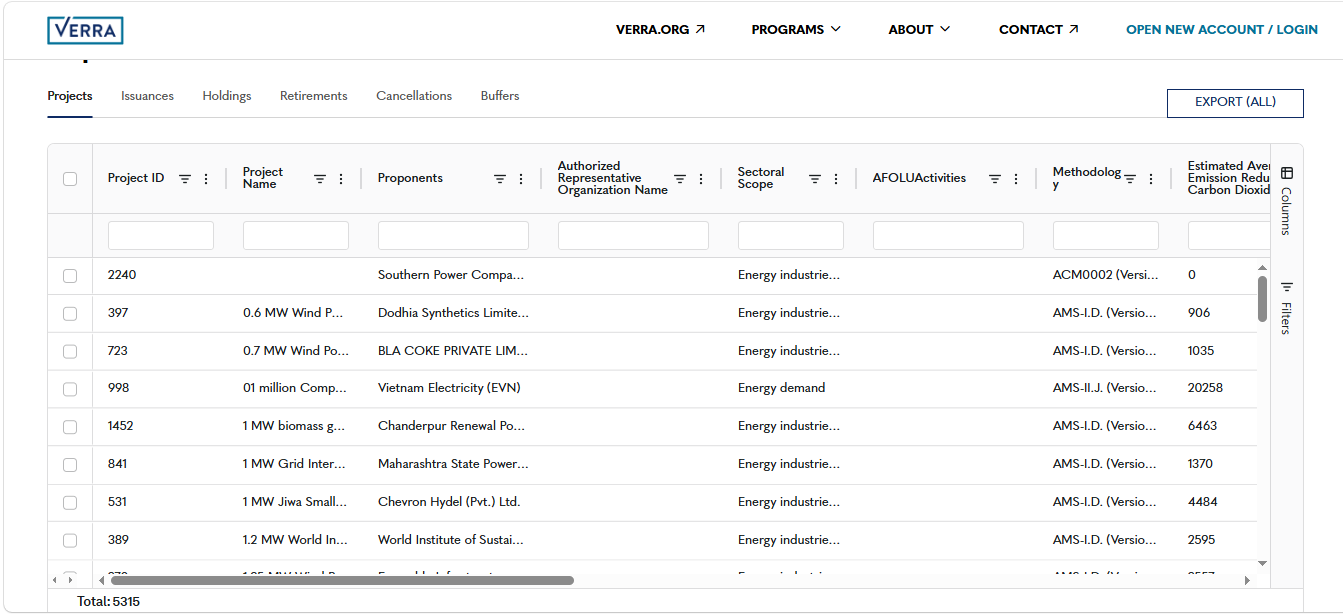
\includegraphics[width=0.85\textwidth]{image/verra_registry.png}
    \caption[Danh sách dự án thuộc chương trình VCS trên Verra Registry]%
    {Danh sách dự án thuộc chương trình VCS trên Verra Registry~\cite{verraregistry}}
    \label{fig:verra}
\end{figure}

National Carbon Credit Registry\index{He thong dang ky@Hệ thống đăng ký (registry)!UNDP National Carbon Registry} của Chương trình phát triển Liên hợp quốc (UNDP) là hệ thống đăng ký quốc gia mã nguồn mở phục vụ Điều~6~\cite{undp2024nationalregistry}. Dữ liệu gốc được ghi trong sổ cái dự án và sổ cái khối tín chỉ, còn PostgreSQL\index{PostgreSQL} chỉ là cơ sở dữ liệu thứ cấp phục vụ truy vấn. Hệ thống chạy trên AWS theo kiến trúc không máy chủ (serverless)\index{Serverless}: hàm Lambda \texttt{national-api} xử lý yêu cầu HTTP, còn hàm \texttt{replicator} được kích hoạt bởi luồng Kinesis để sao chép bản ghi từ sổ cái sang PostgreSQL~\cite{undp2024nationalregistry}. Khi một phần khối tín chỉ (credit block)\index{Khoi tin chi@Khối tín chỉ (Credit Block)} được chuyển nhượng hoặc hủy, hệ thống tách dãy số sê-ri thành hai khối để vẫn truy vết được từng tín chỉ; hệ thống cũng xuất báo cáo theo Định dạng điện tử thỏa thuận (AEF) của Điều~6.2~\cite{undp2024nationalregistry}.

\subsection*{Nền tảng siêu dữ liệu CAD Trust}
\label{subsec:cadtrust}

Climate Action Data Trust (CAD Trust)\index{CAD Trust} không cấp tín chỉ mà là lớp siêu dữ liệu liên kết và chuẩn hóa dữ liệu từ nhiều hệ thống đăng ký như Verra, Gold Standard~\cite{cadtrust2025datamodel}. Mỗi hệ thống đăng ký thành viên chạy một nút của blockchain Chia và tự quản lý dữ liệu của mình; mã băm của mỗi lần cập nhật được ghi lên blockchain để các bên tự đối chiếu và phát hiện dữ liệu bị sửa, còn bản thân dữ liệu nằm trong cơ sở dữ liệu MySQL~\cite{cadtrust2025datamodel}. Mô hình dữ liệu phiên bản 2.0, công bố ngày 23/10/2025, bổ sung các bảng Stakeholders, Methodologies, Validations, Verifications và các bảng AEF cho Điều~6.2 (Bảng~\ref{tab:cadtrust}). Đồ án dùng mô hình CAD Trust V2.0 làm khung cho cơ sở dữ liệu off-chain.

\begin{table}[!htbp]
    \centering
    \caption{Các thực thể dữ liệu chính trong mô hình CAD Trust V2.0}
    \label{tab:cadtrust}
    \small
    \begin{tabularx}{\textwidth}{|L{3.4cm}|Y|}
        \hline
        \HD{Thực thể (bảng)} & \HD{Thuộc tính khóa và mô tả} \\
        \hline
        Project & Mã dự án trên hệ thống đăng ký gốc, chương trình, lĩnh vực, trạng thái; liên kết với Location và Rating \\
        \hline
        Stakeholders & Bảng mới của V2.0: các tổ chức tham gia dự án và vai trò \\
        \hline
        Validations, Verifications & Bảng mới của V2.0: các đợt validation và verification của dự án \\
        \hline
        Issuances & Mỗi bản ghi là một đợt cấp tín chỉ của dự án \\
        \hline
        Units & Khối tín chỉ với dãy số sê-ri, năm vintage\index{Vintage Year}, trạng thái (Issued, Held, Retired); tín chỉ đã hủy có thêm ngày hủy và người thụ hưởng \\
        \hline
        \multicolumn{2}{|l|}{\footnotesize Nguồn: CAD Trust Data Model Version 2.0~\cite{cadtrust2025datamodel}} \\
        \hline
    \end{tabularx}
\end{table}

\subsection*{Khung pháp lý tại Việt Nam}

Văn bản nền tảng là Nghị định 06/2022/NĐ-CP\index{Nghi dinh 06/2022/ND-CP@Nghị định 06/2022/NĐ-CP} về giảm nhẹ phát thải khí nhà kính, đã được sửa đổi bởi các Nghị định 119/2025/NĐ-CP, 83/2026/NĐ-CP, 112/2026/NĐ-CP và 396/2026/NĐ-CP~\cite{vietnam2022nghidinh06}. Nghị định quy định kiểm kê khí nhà kính, phân bổ hạn ngạch\index{Han ngach phat thai@Hạn ngạch phát thải} cho các cơ sở phát thải lớn và cơ chế trao đổi, bù trừ tín chỉ; theo Điều~19 được thay thế bởi Nghị định 119/2025/NĐ-CP, cơ sở được dùng tín chỉ để bù trừ không quá 30\% hạn ngạch được phân bổ~\cite{vietnam2025nghidinh119}. Vì vậy, hệ thống tại Việt Nam phải phân biệt tín chỉ tự nguyện (như VCU) với hạn ngạch và tín chỉ của thị trường trong nước. Hạ tầng của thị trường gồm Hệ thống đăng ký quốc gia\index{He thong dang ky quoc gia@Hệ thống đăng ký quốc gia} theo Thông tư 11/2026/TT-BNNMT~\cite{vietnam2026thongtu11} và sàn giao dịch theo Nghị định 29/2026/NĐ-CP~\cite{vietnam2026nghidinh29}; Nghị định 396/2026/NĐ-CP, có hiệu lực từ ngày 12/12/2026, phân cấp việc cấp tín chỉ theo cơ chế trong nước cho Chủ tịch Ủy ban nhân dân cấp tỉnh~\cite{vietnam2026nghidinh396}. Ngoài thị trường trong nước, năm 2020 Việt Nam ký Thỏa thuận chi trả giảm phát thải (ERPA)\index{ERPA} với Ngân hàng Thế giới, theo đó được chi trả tới 51,5 triệu USD cho 10,3 triệu tấn CO$_2$ giảm phát thải từ rừng tại sáu tỉnh Bắc Trung Bộ đến năm 2025~\cite{worldbank2020erpa}.

% ------------------------------------------------------------
\section{Khảo sát sơ bộ hệ thống}
\label{sec:khaosatsobo}
% Thời gian khảo sát: tháng 9–11/2026 (nguồn truy cập ngày 28/9, 20/10 và 04/11/2026).

\FloatBarrier
\subsection*{Mục tiêu, phạm vi và phương pháp khảo sát}
\label{subsec:ks-gioithieu}

Khảo sát nhằm xác định các bên liên quan, quy trình, dữ liệu và công cụ của các hệ thống đang vận hành, đánh giá ưu, nhược điểm của chúng và rút ra nhu cầu cho hệ thống mới. Phạm vi tập trung vào giai đoạn sau khi tín chỉ được cấp (đăng ký, định danh, chuyển quyền sở hữu, giao dịch, hủy); khâu MRV tại thực địa chỉ được xem ở mức đầu vào. Các hệ thống được khảo sát gồm hạ tầng trong nước (Hệ thống đăng ký quốc gia, hệ thống của sàn giao dịch) và các hệ thống quốc tế (Verra Registry, UNDP National Carbon Registry, CAD Trust, Toucan Protocol).

Do chưa tiếp cận được người dùng thực tế, khảo sát kết hợp hai phương pháp. Nghiên cứu tài liệu dựa trên văn bản pháp luật (nguồn chính thức về quy trình và trách nhiệm của từng bên), tài liệu kỹ thuật của các hệ thống quốc tế và các bài báo khoa học~\cite{kim2020blockchain,sipthorpe2022blockchain,vaccargiu2026blockchain}. Quan sát gồm truy cập trang công khai của các hệ thống không cần đăng nhập, đọc quy trình nội bộ mà cơ quan quản lý đã ban hành và thu thập số liệu vận hành đã công bố. Vì vậy, kết quả chủ yếu phản ánh quy trình theo quy định, chưa phản ánh đầy đủ khó khăn thực tế của người dùng.
% [VIẾT SAU - PHỎNG VẤN] Phỏng vấn 1–2 chuyên gia (đơn vị tư vấn các-bon, công ty chứng khoán thành viên),
% mỗi buổi 20–30 phút. Câu hỏi gợi ý: Q1 (VĐ-1) kiểm tra trùng đăng ký Verra/Gold Standard thế nào;
% Q2 (VĐ-2) chứng minh tín chỉ đã hủy bằng giấy tờ gì; Q3 (VĐ-3) báo cáo thẩm định được lưu, ký thế nào;
% Q4 (VĐ-4) đối soát giữa Hệ thống đăng ký quốc gia, HNX, VSDC tốn bao nhiêu nhân lực; Q5 (VĐ-5) vì sao
% thanh khoản thấp; Q6 dữ liệu nào được phép công khai. Kết quả: bổ sung phương pháp phỏng vấn vào đoạn trên
% và thêm ý kiến chuyên gia vào phần đánh giá.

\FloatBarrier
\subsection*{Hiện trạng hệ thống trong nước}
\label{subsec:ks-tongquan}
\label{subsec:ks-hientrang}

Thị trường tín chỉ các-bon không do một đơn vị duy nhất vận hành (\autoref{fig:mohinhtochuc}). Bộ Nông nghiệp và Môi trường là cơ quan duy nhất cấp mã trong nước và số sê-ri cho hạn ngạch, tín chỉ; Cục Biến đổi khí hậu vận hành Hệ thống đăng ký quốc gia, nơi lưu dữ liệu gốc về chủ sở hữu, số lượng, mã, số sê-ri, trạng thái và lịch sử giao dịch~\cite{vietnam2026thongtu11}. Sở Giao dịch Chứng khoán Hà Nội (HNX)\index{HNX} tổ chức giao dịch, Tổng công ty Lưu ký và Bù trừ Chứng khoán Việt Nam (VSDC)\index{VSDC} phụ trách lưu ký, chuyển quyền sở hữu và thanh toán~\cite{vietnam2026nghidinh29}. Mỗi tổ chức chỉ được cấp một tài khoản đăng ký, gắn với mã số thuế~\cite{vietnam2026thongtu11}. Bảng~\ref{tab:ks-tacnhan} tổng hợp các bên tham gia; Bảng~\ref{tab:ks-hethong} liệt kê các hệ thống được khảo sát.

\HinhMoHinhToChuc

\begin{table}[!htbp]
    \centering
    \caption{Các đối tượng tham gia vòng đời tín chỉ các-bon}
    \label{tab:ks-tacnhan}
    \label{tab:ks-doituong}
    \small
    \begin{tabularx}{\textwidth}{|L{3.3cm}|Y|L{3.8cm}|}
        \hline
        \HD{Đối tượng} & \HD{Vai trò} & \HD{Hệ thống sử dụng} \\
        \hline
        Chủ dự án & Lập hồ sơ, giám sát, nhận và sở hữu tín chỉ & Hệ thống đăng ký quốc gia; Verra Registry \\
        \hline
        Đơn vị thẩm định độc lập (VVB) & Thẩm định hồ sơ và kết quả giảm phát thải theo ISO 14064-3 & Nộp báo cáo cho chương trình hoặc cơ quan cấp \\
        \hline
        Cơ quan quản lý (cấp bộ, cấp tỉnh) & Quyết định cấp tín chỉ, cấp mã và số sê-ri, quản lý tài khoản, đối soát, công bố thông tin & Hệ thống đăng ký quốc gia \\
        \hline
        Cơ sở được phân bổ hạn ngạch & Mua tín chỉ, bù trừ phát thải, nộp trả hạn ngạch & Hệ thống đăng ký quốc gia, tài khoản lưu ký và giao dịch \\
        \hline
        HNX, VSDC, ngân hàng & Tổ chức giao dịch, lưu ký, thanh toán, báo cáo & Hệ thống giao dịch, lưu ký và thanh toán \\
        \hline
        Người dùng công khai & Tra cứu dự án, tín chỉ đã cấp và đã hủy & Thông tin công bố; trang tra cứu Verra Registry \\
        \hline
    \end{tabularx}
\end{table}

\begin{table}[!htbp]
    \centering
    \caption{Các hệ thống đang sử dụng trong vòng đời tín chỉ các-bon}
    \label{tab:ks-hethong}
    \small
    \begin{tabularx}{\textwidth}{|L{3.2cm}|L{2.6cm}|Y|L{2.6cm}|}
        \hline
        \HD{Hệ thống} & \HD{Đơn vị vận hành} & \HD{Chức năng chính} & \HD{Nền tảng} \\
        \hline
        Hệ thống đăng ký quốc gia~\cite{vietnam2026thongtu11} & Cục Biến đổi khí hậu & Tài khoản, mã trong nước, số sê-ri, ký gửi, bù trừ, hủy & Tập trung, xác thực qua Cổng dịch vụ công quốc gia \\
        \hline
        Hệ thống giao dịch, lưu ký~\cite{vietnam2026nghidinh29} & HNX, VSDC & Khớp lệnh, lưu ký, chuyển quyền sở hữu, thanh toán & Tập trung \\
        \hline
        Verra Registry~\cite{verra2024vcs} & Verra & Đăng ký dự án, cấp VCU có số sê-ri, hủy, tra cứu & Tập trung, web \\
        \hline
        UNDP National Carbon Registry~\cite{undp2024nationalregistry} & Từng quốc gia & Đăng ký quốc gia mã nguồn mở, báo cáo AEF & Sổ cái, PostgreSQL trên AWS \\
        \hline
        CAD Trust~\cite{cadtrust2025datamodel} & CAD Trust & Siêu dữ liệu liên thông các hệ thống đăng ký & Blockchain Chia, MySQL \\
        \hline
        Toucan Protocol~\cite{toucan2025docs} & Toucan & Token hóa tín chỉ, pool ERC-20, hủy on-chain & Polygon, Celo \\
        \hline
    \end{tabularx}
\end{table}

Theo Thông tư 11/2026/TT-BNNMT, vòng đời một tín chỉ trên hệ thống trong nước gồm ba nhóm quy trình~\cite{vietnam2026thongtu11,vietnam2026nghidinh29}:
\begin{itemize}
    \item Đăng ký: sau khi cơ quan có thẩm quyền quyết định cấp, trong 05 ngày làm việc Bộ đăng ký tín chỉ (chương trình, cơ chế, số lượng, mã trong nước, chủ sở hữu, số sê-ri) và gửi mã trong nước cho HNX, VSDC.
    \item Ký gửi và giao dịch: chủ tài khoản muốn giao dịch phải ký gửi tín chỉ sang hệ thống lưu ký qua bốn bước:
    \begin{enumerate}
        \item chủ tài khoản thông báo số lượng cần ký gửi; hệ thống chuyển số lượng này từ tiểu khoản Đăng ký chung sang tiểu khoản Chờ ký gửi, hoặc từ chối nếu số dư không đủ;
        \item cuối mỗi ngày làm việc, Bộ tổng hợp danh sách đề nghị ký gửi và gửi cho VSDC;
        \item trong 01 ngày làm việc, VSDC xác nhận hoặc từ chối; khi được xác nhận, số lượng được chuyển sang tiểu khoản Số dư giao dịch;
        \item lệnh được khớp trên hệ thống của HNX; VSDC chuyển quyền sở hữu và thanh toán qua ngân hàng thanh toán.
    \end{enumerate}
    Cuối mỗi ngày, VSDC gửi báo cáo kết quả thanh toán và số dư ký gửi để Bộ đối soát với dữ liệu trên Hệ thống đăng ký quốc gia (Điều~23).
    \item Bù trừ và hủy: tín chỉ bị hủy khi dùng để bù trừ, khi chủ tài khoản hủy tự nguyện (xử lý trong 02 ngày làm việc) hoặc khi bị thu hồi; việc hủy gồm cả số lượng và số sê-ri, và mã trong nước đã hủy không được cấp lại.
\end{itemize}

Dữ liệu cốt lõi là mã trong nước\index{Ma trong nuoc@Mã trong nước} và số sê-ri. Mã của hạn ngạch có dạng VN[năm], ví dụ VN2025; mã của tín chỉ gồm 9 ký tự (mã cơ chế, mã dự án, năm xác nhận); số sê-ri nối mã trong nước với 10 chữ số thứ tự, nên mỗi tấn CO$_2$e có một số sê-ri riêng~\cite{vietnam2026thongtu11}. Mỗi tài khoản có 8 tiểu khoản\index{Tieu khoan@Tiểu khoản} theo Điều~7 Thông tư 11/2026/TT-BNNMT, tương ứng với các trạng thái mà một đơn vị hạn ngạch hoặc tín chỉ có thể đi qua (Bảng~\ref{tab:ks-tieukhoan}); khi đổi trạng thái, số lượng được chuyển giữa các tiểu khoản, và các nghiệp vụ ký gửi, chuyển quyền sở hữu, chuyển giao, vay mượn chỉ thực hiện được với số lượng đang ở tiểu khoản Đăng ký chung~\cite{vietnam2026thongtu11}.

\begin{table}[!htbp]
    \centering
    \caption{Các tiểu khoản của tài khoản đăng ký theo Thông tư 11/2026/TT-BNNMT}
    \label{tab:ks-tieukhoan}
    \begin{tabularx}{\textwidth}{|L{3.2cm}|Y|}
        \hline
        \HD{Tiểu khoản} & \HD{Nội dung ghi nhận} \\
        \hline
        Đăng ký chung & Hạn ngạch, tín chỉ thuộc sở hữu hợp pháp của chủ tài khoản, chưa đưa vào giao dịch hay nghiệp vụ khác \\
        \hline
        Chờ ký gửi & Hạn ngạch, tín chỉ đã đề nghị ký gửi, đang chờ VSDC xác nhận \\
        \hline
        Số dư giao dịch & Hạn ngạch, tín chỉ đã ký gửi tại VSDC \\
        \hline
        Bù trừ & Tín chỉ được dùng để bù trừ phát thải \\
        \hline
        Nộp trả & Hạn ngạch được chủ tài khoản nộp trả \\
        \hline
        Chuyển giao & Hạn ngạch chuyển từ giai đoạn hiện tại sang giai đoạn kế tiếp \\
        \hline
        Vay mượn & Hạn ngạch của giai đoạn kế tiếp được vay để dùng cho giai đoạn hiện tại \\
        \hline
        Phong tỏa & Hạn ngạch, tín chỉ bị phong tỏa theo yêu cầu của cơ quan có thẩm quyền \\
        \hline
        \multicolumn{2}{|l|}{\footnotesize Nguồn: Điều~7 Thông tư 11/2026/TT-BNNMT~\cite{vietnam2026thongtu11}} \\
        \hline
    \end{tabularx}
\end{table}

Về công bố thông tin, Bộ công bố hằng tháng (chậm nhất ngày 20 tháng sau) danh sách dự án đã đăng ký và tổng số lượng đăng ký mới, hủy đăng ký, đồng thời công bố trong vòng 72 giờ việc cấp, hủy mã trong nước và số sê-ri; thông tin truy cập và thông tin giao dịch của các tổ chức phải được bảo mật~\cite{vietnam2026thongtu11}. Các công cụ hỗ trợ gồm xác thực qua Cổng dịch vụ công quốc gia, cơ chế một người tạo và một người khác duyệt mỗi giao dịch, kết nối với HNX, VSDC qua kênh riêng hoặc API mã hóa, và công bố thông tin định kỳ theo tháng, năm~\cite{vietnam2026thongtu11}.

\FloatBarrier
\subsection*{Quan sát các hệ thống thực tế}
\label{subsec:ks-quansat}

Để kiểm tra các nhận định rút ra từ văn bản, đồ án truy cập trang công khai của một số hệ thống ngày 04/11/2026. Bảng~\ref{tab:ks-quansat} tóm tắt kết quả; \autoref{fig:ks-dvc-taikhoan} đến \autoref{fig:ks-toucan} là ảnh chụp màn hình các trang được quan sát.

\begin{table}[!htbp]
    \centering
    \caption{Kết quả quan sát các hệ thống thực tế}
    \label{tab:ks-quansat}
    \label{tab:ks-quansat-qt}
    \small
    \begin{tabularx}{\textwidth}{|L{3.0cm}|Y|}
        \hline
        \HD{Hệ thống} & \HD{Kết quả ghi nhận} \\
        \hline
        Thủ tục đăng ký tài khoản (mã 1.014129) & Hồ sơ nộp trực tiếp, trực tuyến hoặc qua bưu chính; thời hạn 05 ngày làm việc; hồ sơ qua chuyên viên, lãnh đạo phòng, lãnh đạo Cục và lãnh đạo Bộ duyệt~\cite{mae2026tthc1014129,mae2025qd2935} \\
        \hline
        Thủ tục cấp tín chỉ trong nước (mã 1.014133) & Trang thủ tục vẫn hiển thị quy trình cũ: bộ quản lý lĩnh vực quyết định, tổng 06 ngày làm việc và 30 ngày, có nhánh bổ sung hồ sơ~\cite{mae2026tthc1014133}; từ ngày 12/12/2026, Chủ tịch Ủy ban nhân dân cấp tỉnh quyết định trong tối đa 26 ngày làm việc~\cite{vietnam2026nghidinh396} \\
        \hline
        Sàn giao dịch các-bon (HNX) & VN2025 là mã duy nhất (511.473.846 tấn CO$_2$e hạn ngạch, giao dịch từ 29/6/2026 đến 24/12/2027)~\cite{hnx2026vn2025,hnx2026danhmuchanngach}; khối lượng giao dịch theo tháng rất nhỏ, chưa có tín chỉ nào được giao dịch~\cite{hnx2026sanphamcacbon}; trang thống kê giao dịch chưa công bố số liệu tổng hợp~\cite{hnx2026ketquagd} \\
        \hline
        Verra Registry & Ai cũng tra cứu được, nhưng phát hành, chuyển nhượng, hủy cần tài khoản; báo cáo Retirements công khai từng lô với ngày hủy, dự án, vintage, số sê-ri; người thụ hưởng và lý do hủy có thể ẩn~\cite{verraregistry,verra2020registryv2} \\
        % [VIẾT SAU - SỐ LIỆU] Lọc Retirement Date = 04/11/2026, ghi tổng số lô được hủy trong ngày.
        \hline
        CAD Trust & Dashboard công khai chỉ có số liệu tổng hợp theo khu vực, quốc gia; không tìm thấy trang chi tiết dự án khi không đăng nhập~\cite{cadtrust2026dashboard} \\
        % [VIẾT SAU - ẢNH CHỤP] Chọn Southeast Asia -> Viet Nam trên dashboard, ghi số dự án và nội dung ô Registry.
        \hline
        Toucan Protocol & Trang dự án Wakefield Biochar Facility 2 giữ mã dự án PUR-244045 của tiêu chuẩn gốc Puro và cho biết tín chỉ đã nằm trong pool CHAR~\cite{toucan2026wakefield} \\
        \hline
    \end{tabularx}
\end{table}

\begin{figure}[!htbp]
    \centering
    \begin{subfigure}{\textwidth}
        \centering
        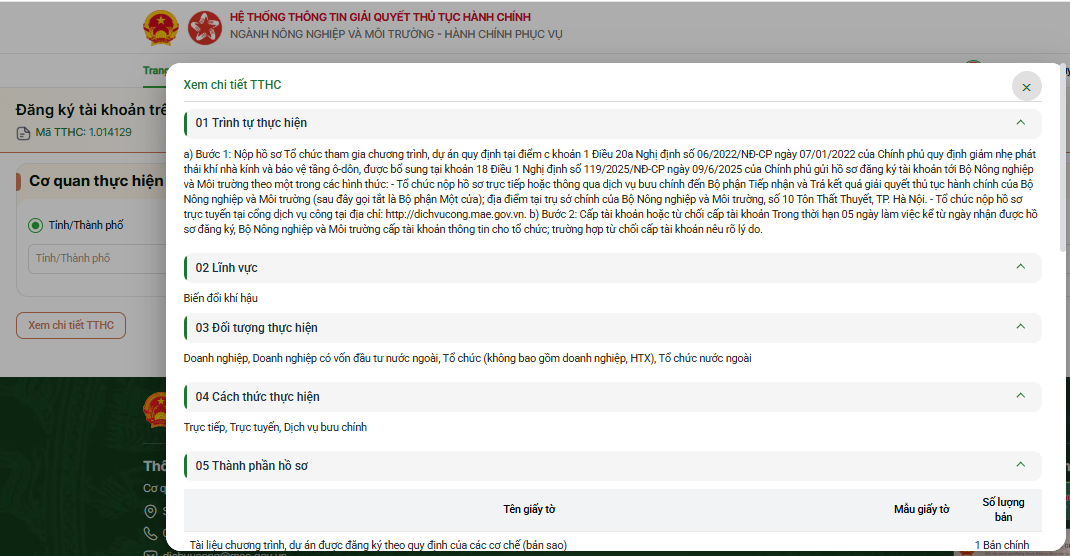
\includegraphics[width=0.8\textwidth]{image/dvc_1014129_trinh_tu.png}
        \caption{Trình tự thực hiện}
    \end{subfigure}

    \vspace{0.3cm}
    \begin{subfigure}{\textwidth}
        \centering
        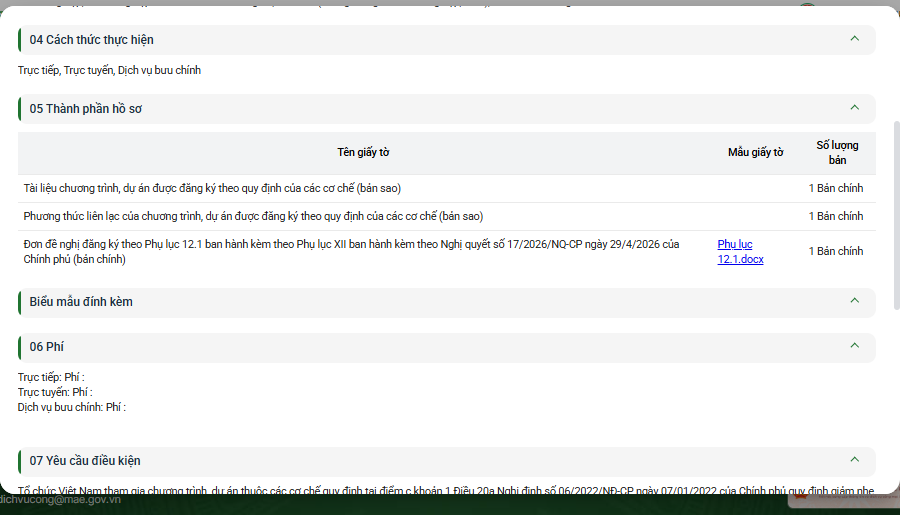
\includegraphics[width=0.68\textwidth]{image/dvc_1014129_ho_so.png}
        \caption{Thành phần hồ sơ}
    \end{subfigure}

    \vspace{0.3cm}
    \begin{subfigure}{\textwidth}
        \centering
        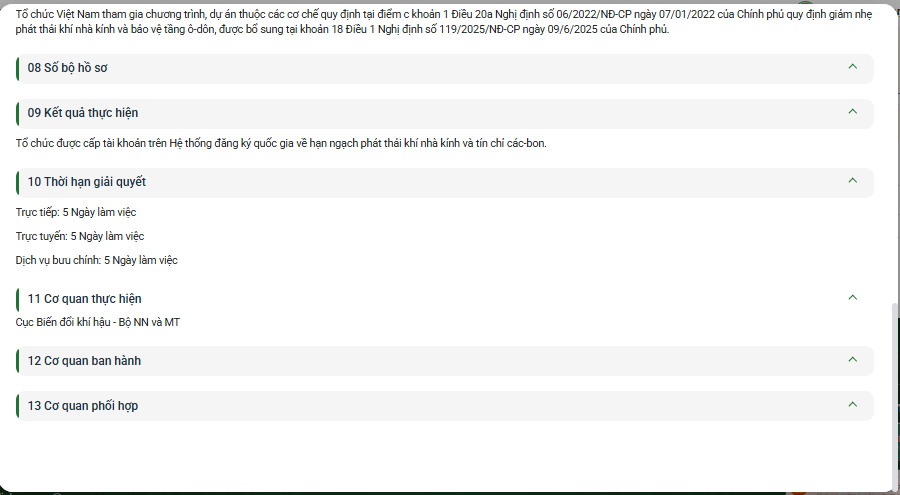
\includegraphics[width=0.68\textwidth]{image/dvc_1014129_thoi_han.png}
        \caption{Kết quả, thời hạn giải quyết và cơ quan thực hiện}
    \end{subfigure}
    \caption[Trang thủ tục đăng ký tài khoản trên Hệ thống đăng ký quốc gia]%
    {Trang thủ tục mã 1.014129 về đăng ký tài khoản trên Hệ thống đăng ký quốc gia (truy cập ngày 04/11/2026)~\cite{mae2026tthc1014129}}
    \label{fig:ks-dvc-taikhoan}
\end{figure}

\begin{figure}[!htbp]
    \centering
    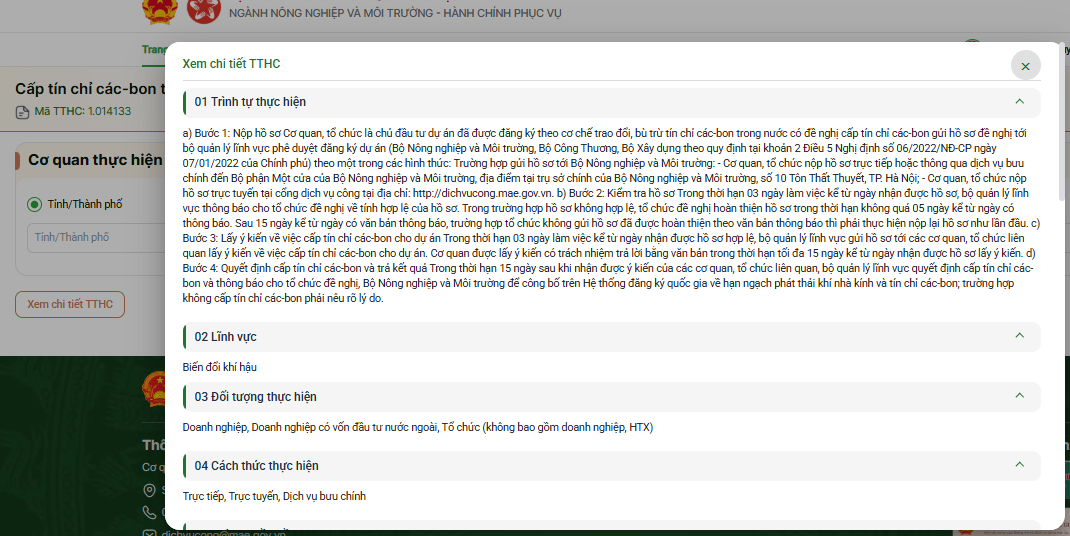
\includegraphics[width=0.85\textwidth]{image/dvc_1014133_trinh_tu.png}
    \caption[Trang thủ tục cấp tín chỉ các-bon theo cơ chế trong nước]%
    {Trang thủ tục mã 1.014133 về cấp tín chỉ các-bon theo cơ chế trong nước, trình tự bốn bước trước Nghị định 396/2026/NĐ-CP (truy cập ngày 04/11/2026)~\cite{mae2026tthc1014133}}
    \label{fig:ks-dvc-tinchi}
\end{figure}

\begin{figure}[!htbp]
    \centering
    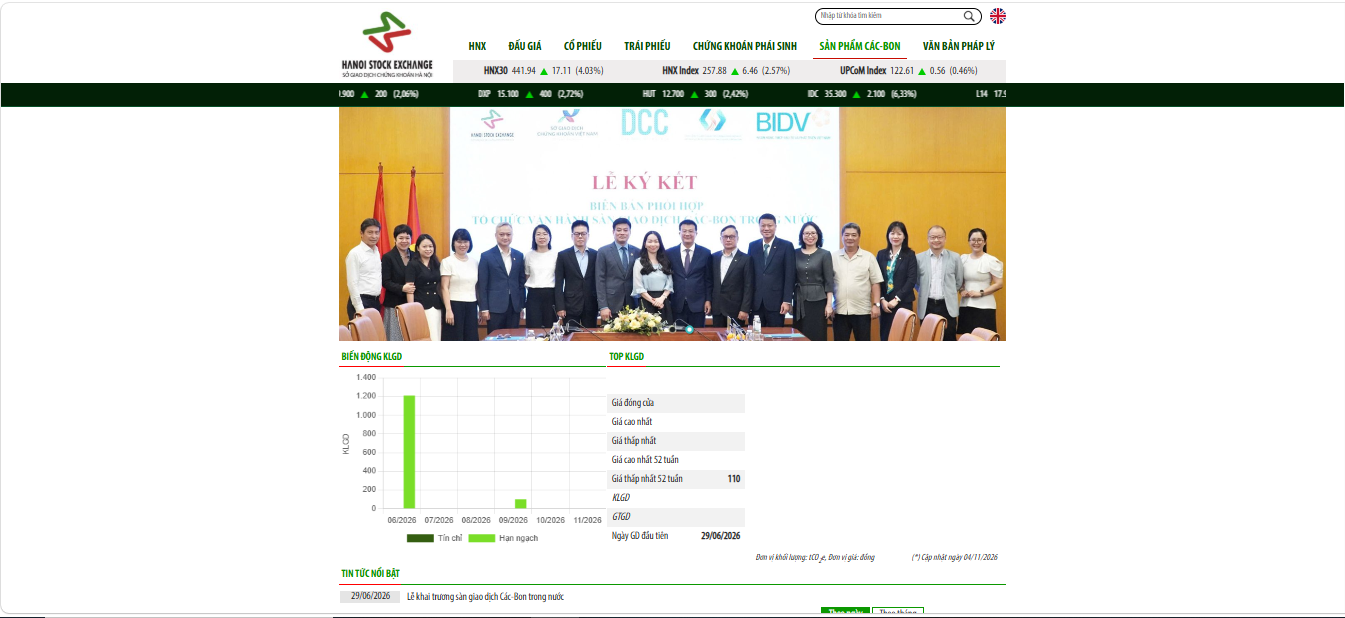
\includegraphics[width=0.9\textwidth]{image/hnx_san_cacbon.png}
    \caption[Trang sản phẩm các-bon trên website của HNX]%
    {Trang sản phẩm các-bon của HNX: khối lượng giao dịch theo tháng và thông tin mã VN2025 (truy cập ngày 04/11/2026)~\cite{hnx2026sanphamcacbon}}
    \label{fig:ks-hnx}
\end{figure}

\begin{figure}[!htbp]
    \centering
    \begin{subfigure}{\textwidth}
        \centering
        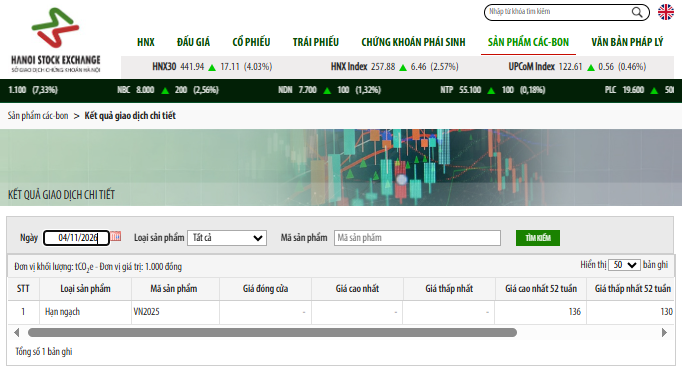
\includegraphics[width=0.75\textwidth]{image/hnx_ket_qua_giao_dich.png}
        \caption{Kết quả giao dịch chi tiết ngày 04/11/2026~\cite{hnx2026ketquagd}}
    \end{subfigure}

    \vspace{0.3cm}
    \begin{subfigure}{\textwidth}
        \centering
        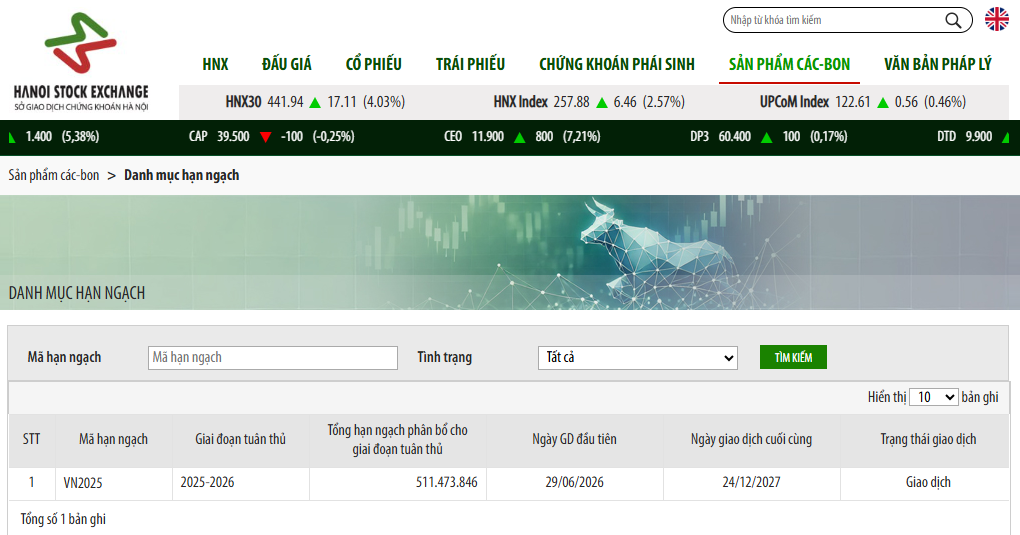
\includegraphics[width=0.85\textwidth]{image/hnx_danh_muc_han_ngach.png}
        \caption{Danh mục hạn ngạch~\cite{hnx2026danhmuchanngach}}
    \end{subfigure}
    \caption[Kết quả giao dịch và danh mục hạn ngạch trên website của HNX]%
    {Kết quả giao dịch và danh mục hạn ngạch trên trang sản phẩm các-bon của HNX (truy cập ngày 04/11/2026)}
    \label{fig:ks-hnx-chitiet}
\end{figure}

\begin{figure}[!htbp]
    \centering
    \begin{subfigure}{\textwidth}
        \centering
        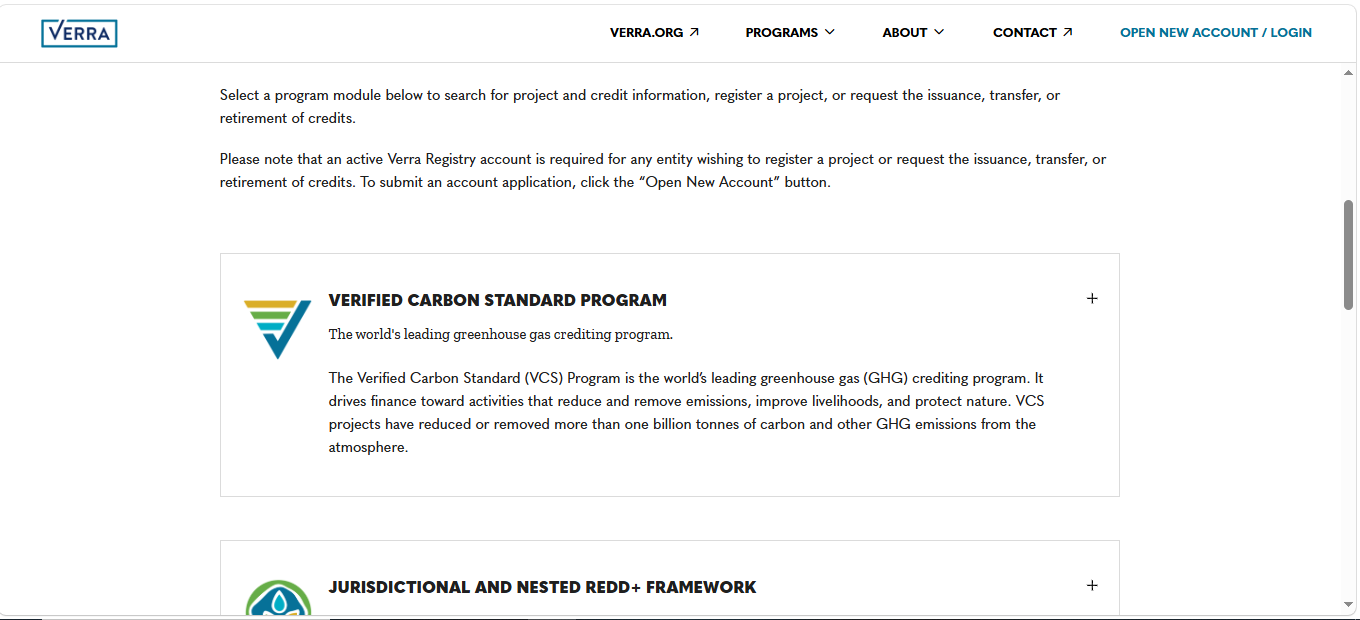
\includegraphics[width=0.85\textwidth]{image/verra_registry_home.png}
        \caption{Trang chủ: tra cứu theo chương trình là công khai, còn đăng ký, phát hành, chuyển nhượng và hủy tín chỉ yêu cầu tài khoản~\cite{verraregistry}}
    \end{subfigure}

    \vspace{0.3cm}
    \begin{subfigure}{\textwidth}
        \centering
        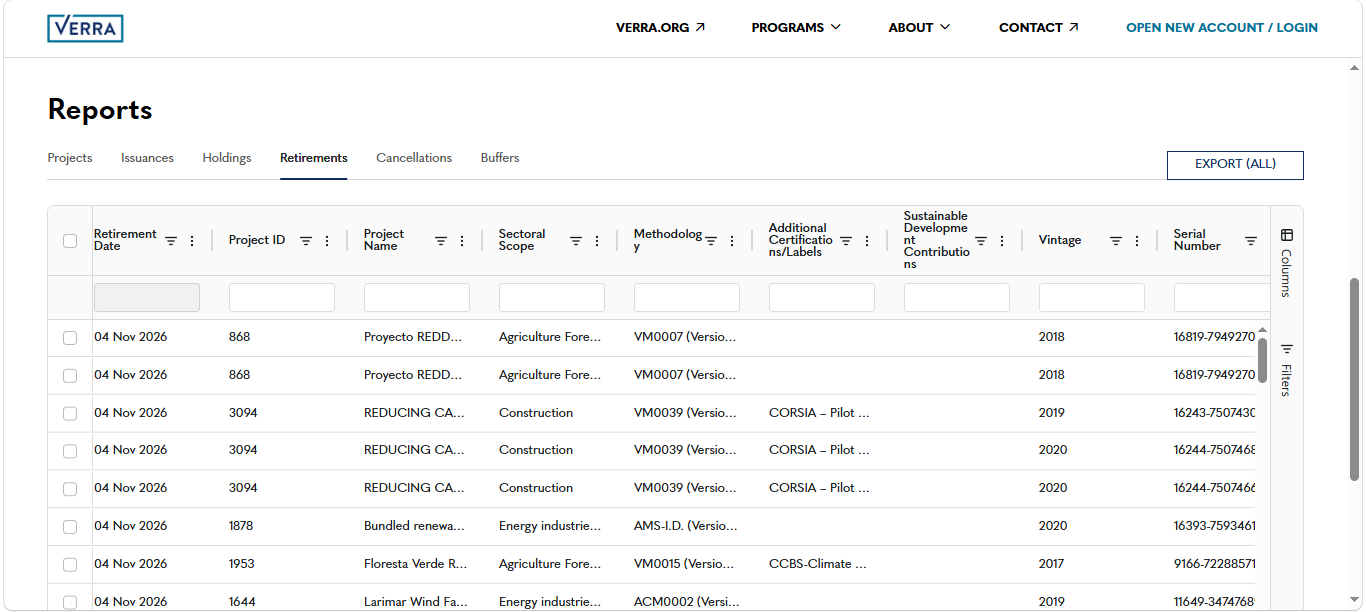
\includegraphics[width=0.85\textwidth]{image/verra_retirements.png}
        \caption{Báo cáo Retirements: mỗi dòng là một lô tín chỉ đã hủy, có ngày hủy, dự án, vintage và số sê-ri~\cite{verraregistry}}
    \end{subfigure}
    \caption[Trang công khai của Verra Registry]%
    {Trang công khai của Verra Registry (truy cập ngày 04/11/2026)}
    \label{fig:ks-verra}
\end{figure}

% [VIẾT SAU - ẢNH CHỤP] Thay bằng ảnh dashboard của Việt Nam (Southeast Asia -> Viet Nam) và sửa chú thích.
\begin{figure}[!htbp]
    \centering
    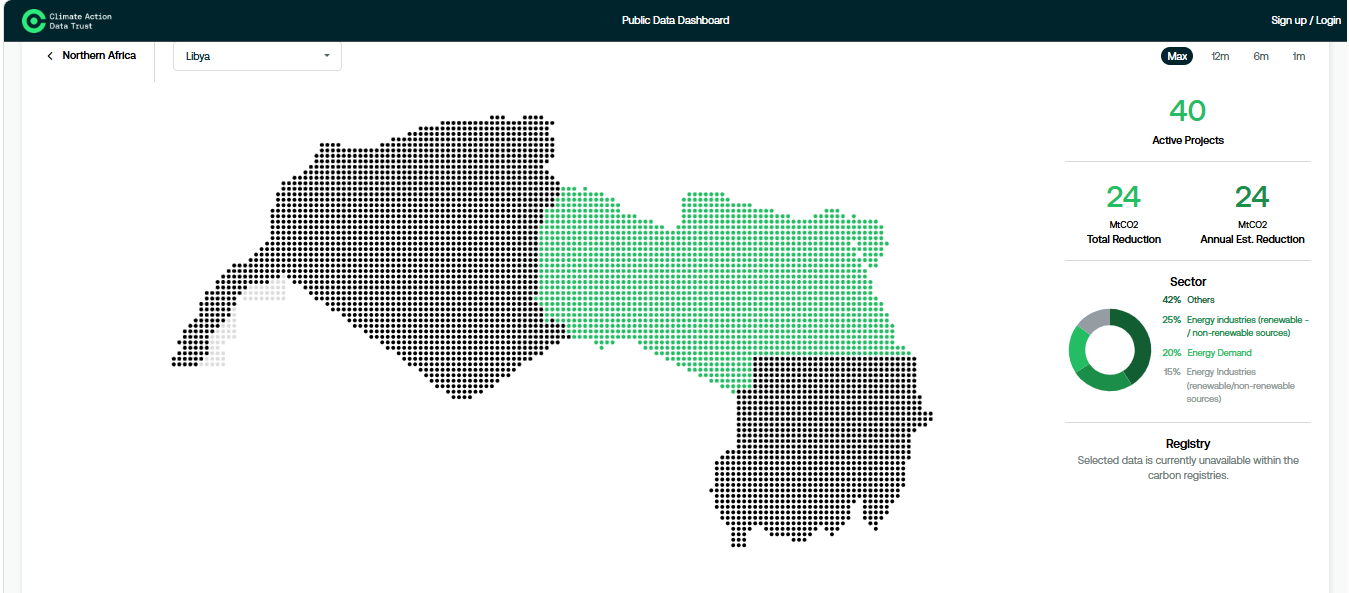
\includegraphics[width=0.85\textwidth]{image/cadtrust_dashboard.png}
    \caption[Public Data Dashboard của CAD Trust]%
    {Public Data Dashboard của CAD Trust: số liệu tổng hợp của một quốc gia gồm số dự án, lượng giảm phát thải và cơ cấu theo lĩnh vực (truy cập ngày 04/11/2026)~\cite{cadtrust2026dashboard}}
    \label{fig:ks-cadtrust}
\end{figure}

\begin{figure}[!htbp]
    \centering
    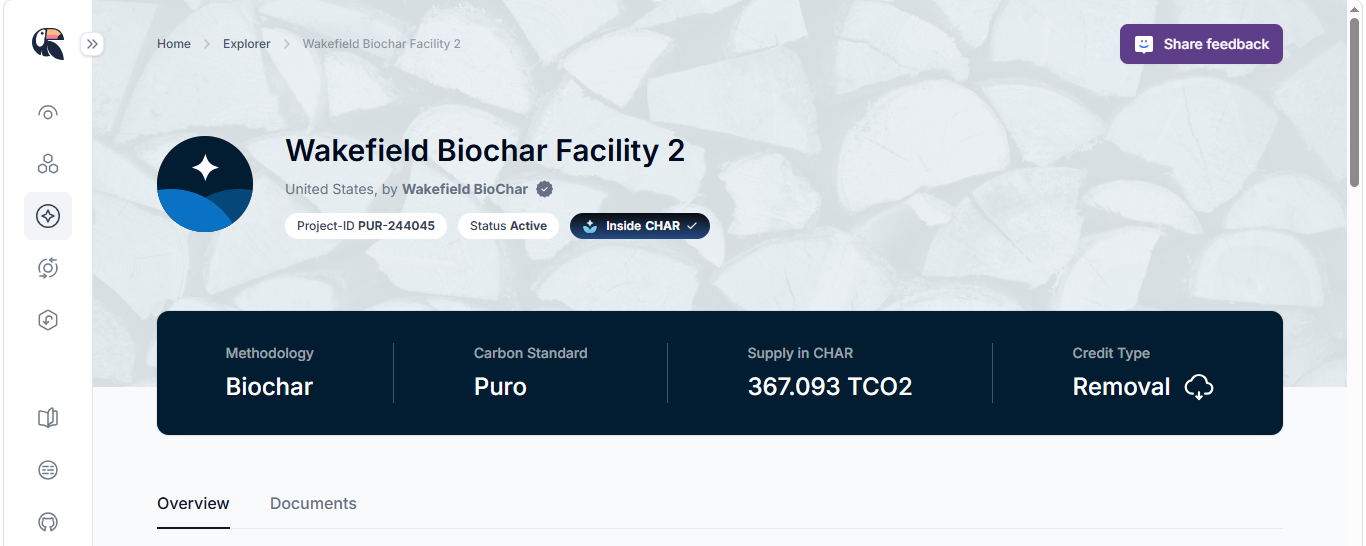
\includegraphics[width=0.85\textwidth]{image/toucan_project.png}
    \caption[Trang một dự án trên ứng dụng Toucan]%
    {Trang dự án Wakefield Biochar Facility 2 trên ứng dụng Toucan: mã dự án, tiêu chuẩn gốc, phương pháp luận, loại tín chỉ và pool chứa token (truy cập ngày 04/11/2026)~\cite{toucan2026wakefield}}
    \label{fig:ks-toucan}
\end{figure}

Từ kết quả quan sát rút ra bốn nhận xét.

Thứ nhất, nghiệp vụ trong nước đi qua nhiều cấp phê duyệt và nhiều hệ thống: một giao dịch cần dữ liệu ở Hệ thống đăng ký quốc gia, hệ thống giao dịch của HNX, hệ thống lưu ký của VSDC và tài khoản tại công ty chứng khoán. Mỗi bước của thủ tục cấp tín chỉ có thời hạn riêng và có nhánh quay lại khi hồ sơ phải bổ sung. Theo Nghị định 396/2026/NĐ-CP, từ ngày 12/12/2026 việc cấp tín chỉ trong nước mất tối đa 26 ngày làm việc, so với khoảng 27 đến 28 ngày làm việc của quy trình cũ~\cite{vietnam2026nghidinh396}. Thay đổi lớn hơn là thẩm quyền được phân cấp xuống cấp tỉnh: tín chỉ sẽ được cấp ở nhiều địa phương nhưng vẫn phải ghi nhận thống nhất trên Hệ thống đăng ký quốc gia, nên hệ thống mới cần cho phép nhiều tài khoản cùng có quyền phát hành (NC-09).

Thứ hai, thị trường chưa có thanh khoản: đến ngày 04/11/2026 hàng hóa duy nhất là hạn ngạch, nên chưa có dữ liệu thực tế về giao dịch tín chỉ trong nước để hệ thống của đồ án sử dụng.

Thứ ba, Verra Registry tách rõ phần tra cứu công khai và phần nghiệp vụ cần tài khoản; báo cáo hủy tín chỉ công khai tới từng lô và số sê-ri nhưng thông tin người thụ hưởng có thể được ẩn, cho thấy yêu cầu minh bạch luôn đi kèm giới hạn về riêng tư.

Thứ tư, các hệ thống tổng hợp dữ liệu hoặc token hóa tín chỉ đều dựa vào hệ thống đăng ký gốc: CAD Trust chỉ hiển thị được số liệu mà các hệ thống đăng ký cung cấp, còn dự án được quan sát trên Toucan là tín chỉ do Puro cấp và vẫn giữ mã dự án của Puro. Vì vậy, mỗi bản ghi tín chỉ trên blockchain cần giữ liên kết tới mã dự án và số sê-ri do hệ thống đăng ký gốc cấp.

\FloatBarrier
\subsection*{Đánh giá hệ thống hiện tại}
\label{subsec:ks-danhgia}

Hệ thống trong nước có cơ sở pháp lý rõ ràng, dữ liệu gốc thống nhất, số sê-ri tới từng tấn CO$_2$e, mô hình tám tiểu khoản chặt chẽ và định danh pháp lý qua Cổng dịch vụ công quốc gia; các hệ thống quốc tế đóng góp các ý tưởng như tra cứu công khai (Verra), mã nguồn mở và tách khối sê-ri (UNDP), mô hình dữ liệu chung (CAD Trust) và hủy tín chỉ công khai trên blockchain (Toucan). Bảng~\ref{tab:ks-uunhuoc} tóm tắt ưu, nhược điểm của từng hệ thống.

\begin{table}[!htbp]
    \centering
    \caption{Ưu điểm và nhược điểm của các hệ thống được khảo sát}
    \label{tab:ks-uunhuoc}
    \small
    \begin{tabularx}{\textwidth}{|L{2.8cm}|Y|Y|}
        \hline
        \HD{Hệ thống} & \HD{Ưu điểm} & \HD{Nhược điểm} \\
        \hline
        Hệ thống trong nước & Pháp lý rõ ràng; dữ liệu gốc thống nhất; số sê-ri tới từng đơn vị; xác thực định danh điện tử & Đang thí điểm; ba hệ thống phải đối soát cuối ngày; công khai chủ yếu ở dạng tổng hợp; bên ngoài không tự kiểm chứng được lịch sử tín chỉ \\
        \hline
        Verra Registry & Quy mô lớn; số sê-ri duy nhất; tra cứu công khai & Tập trung; chưa có API công khai; không liên thông với hệ thống khác \\
        \hline
        UNDP National Carbon Registry & Mã nguồn mở; hỗ trợ Điều~6 và AEF; tách dãy sê-ri & Mỗi quốc gia tự vận hành hạ tầng; sổ cái do một bên quản lý \\
        \hline
        CAD Trust & Liên thông nhiều hệ thống; mô hình dữ liệu chung; mã băm trên blockchain & Không ghi quyền sở hữu, không giao dịch; mã băm chứng minh dữ liệu không bị sửa, không chứng minh dữ liệu đúng \\
        \hline
        Toucan Protocol & Hủy tín chỉ và chứng nhận hủy công khai on-chain & Phụ thuộc hệ thống đăng ký gốc; Verra đã cấm token hóa tín chỉ đã hủy~\cite{verra2022crypto}; pool làm mất thông tin riêng của dự án \\
        \hline
    \end{tabularx}
\end{table}

Đối với hệ thống trong nước, các nhược điểm chính là:
\begin{itemize}
    \item Tính toàn vẹn dựa vào niềm tin vào đơn vị vận hành: các ràng buộc như mã trong nước không được cấp lại sau khi hủy hay không hủy quá số dư được bảo đảm bởi phần mềm và quy trình của cơ quan quản lý; bên mua hoặc tổ chức bên ngoài không có công cụ để tự kiểm chứng rằng một số sê-ri chưa từng được cấp cho người khác hoặc chưa từng bị hủy.
    \item Dữ liệu phân tán giữa nhiều hệ thống: cùng một lượng tín chỉ được ghi ở Hệ thống đăng ký quốc gia và ở hệ thống lưu ký của VSDC, nên phải đối soát cuối mỗi ngày và có quy trình xử lý sai lệch~\cite{vietnam2026thongtu11}.
    \item Độ trễ trong nghiệp vụ: ký gửi chờ tổng hợp cuối ngày và chờ VSDC xác nhận trong 01 ngày làm việc; hủy tự nguyện được xử lý trong 02 ngày làm việc~\cite{vietnam2026thongtu11}.
    \item Mức độ công khai hạn chế: dữ liệu công bố chủ yếu là số liệu tổng hợp theo tháng, năm, còn thông tin giao dịch được bảo mật; điều này phù hợp yêu cầu bảo mật nhưng khiến bên thứ ba khó truy vết lịch sử của một tín chỉ cụ thể, và tại thời điểm khảo sát chưa có tài liệu API công khai cho bên thứ ba.
    \item Khâu MRV chưa được số hóa đồng bộ: hồ sơ dự án, báo cáo giám sát và báo cáo thẩm định vẫn là các tệp được nộp qua từng bước, chưa gắn với tín chỉ được cấp bằng một dấu vết kiểm chứng được~\cite{mae2026tthc1014133}.
\end{itemize}

Từ các nhược điểm trên, đồ án xác định năm vấn đề làm cơ sở cho nhu cầu của hệ thống mới:
\begin{enumerate}[label=VĐ-\arabic*., leftmargin=1.6cm]
    \item Rủi ro phát hành kép giữa các hệ thống: hệ thống trong nước và các chương trình quốc tế dùng không gian định danh khác nhau; nếu không liên thông dữ liệu, một dự án có thể được đăng ký ở nhiều nơi~\cite{schneider2019double}.
    \item Bên mua khó chứng minh tín chỉ đã được hủy: bằng chứng hiện nay chủ yếu là thông báo xác nhận do cơ quan quản lý gửi cho chủ tài khoản, bên thứ ba không tự kiểm tra được.
    \item Hồ sơ MRV và thẩm định không gắn chặt với tín chỉ: không có cơ chế kỹ thuật bảo đảm hồ sơ không bị sửa sau khi cấp hoặc không bị dùng lại cho lần cấp khác.
    \item Chi phí đối soát giữa nhiều cơ sở dữ liệu: cùng một lượng tín chỉ được ghi ở ba hệ thống, các bên phải đối soát cuối mỗi ngày và duy trì quy trình xử lý sai lệch~\cite{vietnam2026thongtu11}.
    \item Thị trường còn ở giai đoạn đầu và quy định đang thay đổi (ví dụ phân cấp cho cấp tỉnh theo Nghị định 396/2026/NĐ-CP~\cite{vietnam2026nghidinh396}), nên hệ thống mới cần linh hoạt về phân quyền.
\end{enumerate}

\FloatBarrier
\subsection*{Nhu cầu xây dựng hệ thống mới}
\label{subsec:ks-nhucau}

Hệ thống mới không thay thế Hệ thống đăng ký quốc gia mà là một nguyên mẫu bổ sung: thử nghiệm việc biến các ràng buộc nghiệp vụ đã được quy định (số sê-ri duy nhất, không hủy hai lần, không chuyển nhượng tín chỉ đã hủy) thành ràng buộc kỹ thuật mà ai cũng kiểm chứng được. Bảng~\ref{tab:ks-nhucauchucnang} liệt kê các nhu cầu chức năng; ``một phần'' nghĩa là nhu cầu chỉ giải quyết vấn đề trong phạm vi hệ thống, dấu ``--'' nghĩa là nhu cầu phục vụ vận hành.

\begin{table}[!htbp]
    \centering
    \caption{Nhu cầu chức năng của hệ thống mới}
    \label{tab:ks-nhucauchucnang}
    \small
    \begin{tabularx}{\textwidth}{|L{1.3cm}|Y|L{2.8cm}|L{2.1cm}|}
        \hline
        \HD{Mã} & \HD{Nhu cầu} & \HD{Bên liên quan} & \HD{Vấn đề} \\
        \hline
        NC-01 & Đăng ký dự án, tải lên hồ sơ (PDD, báo cáo giám sát), lưu mã băm hồ sơ & Chủ dự án & VĐ-3 \\
        \hline
        NC-02 & Gửi yêu cầu cấp tín chỉ; VVB phê duyệt hoặc từ chối & Chủ dự án, VVB & VĐ-3 \\
        \hline
        NC-03 & Phát hành lô tín chỉ có dãy sê-ri duy nhất; từ chối dãy sê-ri trùng hoặc hồ sơ đã dùng & Cơ quan quản lý & VĐ-1 (một phần), VĐ-3 \\
        \hline
        NC-04 & Chuyển nhượng tín chỉ giữa các ví, ghi lịch sử sở hữu công khai & Chủ dự án, doanh nghiệp & VĐ-2, VĐ-4 \\
        \hline
        NC-05 & Giao dịch từng phần của một lô qua pool token có thể thay thế & Chủ dự án, doanh nghiệp & -- \\
        \hline
        NC-06 & Hủy tín chỉ từ lô hoặc từ pool, ghi người thụ hưởng và dãy sê-ri bị hủy; tín chỉ đã hủy không chuyển nhượng hay hủy lại được & Doanh nghiệp & VĐ-2 \\
        \hline
        NC-07 & Tra cứu công khai theo số sê-ri, xem chứng nhận hủy kèm liên kết giao dịch on-chain & Người dùng công khai & VĐ-2 \\
        \hline
        NC-08 & Dashboard so sánh tín chỉ đã hủy với lượng phát thải hoặc hạn ngạch khai báo & Doanh nghiệp & VĐ-2 \\
        \hline
        NC-09 & Quản lý vai trò VVB và phát hành; nhiều tài khoản cùng có quyền phát hành (mỗi tỉnh một tài khoản), ghi tài khoản đã phát hành từng lô; tạm dừng khi có sự cố & Cơ quan quản lý & VĐ-5 \\
        \hline
        NC-10 & Xuất dữ liệu dự án, đợt cấp, đơn vị tín chỉ theo cấu trúc CAD Trust V2.0 & Cơ quan quản lý, hệ thống ngoài & VĐ-1 (một phần) \\
        \hline
    \end{tabularx}
\end{table}

Các nhu cầu phi chức năng gồm:
\begin{itemize}
    \item Toàn vẹn và kiểm chứng được: mỗi dãy sê-ri chỉ phát hành một lần; quyền sở hữu và trạng thái hủy lấy dữ liệu on-chain làm gốc; bên thứ ba tự kiểm tra được lịch sử của một tín chỉ.
    \item Bảo mật và riêng tư: chỉ vai trò phù hợp mới được phát hành hoặc đổi vai trò; smart contract chống các lỗ hổng phổ biến như reentrancy. Để dung hòa yêu cầu công khai (Điều~4) và bảo mật thông tin giao dịch (Điều~24) của Thông tư 11/2026/TT-BNNMT~\cite{vietnam2026thongtu11}, on-chain chỉ ghi địa chỉ ví, dãy sê-ri, trạng thái và mã băm hồ sơ; thông tin định danh doanh nghiệp, hồ sơ và giá giao dịch lưu off-chain có phân quyền, tương tự cách làm của CAD Trust và Verra~\cite{cadtrust2025datamodel,verra2020registryv2}.
    \item Chi phí và tương thích: chi phí gas của các thao tác chính được đo và ở mức chấp nhận được; dữ liệu off-chain theo mô hình CAD Trust V2.0; kiến trúc tách lớp để mở rộng (ký số của VVB, kết nối MRV, ánh xạ sang mã trong nước).
\end{itemize}

Định hướng giải pháp là kiến trúc lai on-chain và off-chain. Ba thao tác cần kiểm chứng công khai (phát hành, chuyển nhượng, hủy) được thực hiện bằng smart contract trên Ethereum: mỗi lô tín chỉ là một NFT ERC-721 lưu dãy sê-ri và mã băm hồ sơ, pool ERC-20 phục vụ giao dịch từng phần, hàm hủy đốt token và ghi người thụ hưởng. Hồ sơ, dự án và tài khoản được lưu trong cơ sở dữ liệu quan hệ, cập nhật từ sự kiện on-chain. Thiết kế giữ lại các ý tưởng của hệ thống trong nước: định danh theo lô với dãy sê-ri, tách người tạo và người duyệt, VVB chỉ phê duyệt kết quả thẩm định còn cơ quan quản lý mới phát hành~\cite{mae2025qd2935,vietnam2026nghidinh396}, và khả năng tạm dừng hệ thống khi có sự cố.
% [VIẾT SAU] Khi khôi phục Chương 3: thêm "(mục \ref{sec:kientruc})" sau "kiến trúc lai on-chain và off-chain".

\FloatBarrier
\subsection*{Kết luận và đánh giá tính khả thi sơ bộ}
\label{subsec:ks-khathi}

Việt Nam đã có hạ tầng pháp lý và kỹ thuật tương đối đầy đủ cho thị trường các-bon trong nước. Khoảng trống mà đồ án hướng tới không phải là việc thiếu một hệ thống quản lý, mà là việc các ràng buộc chống tính toán kép đang dựa vào niềm tin vào đơn vị vận hành và đối soát giữa nhiều cơ sở dữ liệu. Bảng~\ref{tab:ks-khathi} cho thấy việc xây dựng hệ thống ở mức nguyên mẫu là khả thi trong thời gian của đồ án; các nhu cầu ở trên là đầu vào cho phần phân tích yêu cầu ở các chương sau.
% [VIẾT SAU] Khi khôi phục Chương 3: "ở Chương~\ref{chap:thietke}" thay cho "ở các chương sau".

\begin{table}[!htbp]
    \centering
    \caption{Đánh giá tính khả thi sơ bộ}
    \label{tab:ks-khathi}
    \small
    \begin{tabularx}{\textwidth}{|L{2.2cm}|Y|Y|}
        \hline
        \HD{Khía cạnh} & \HD{Đánh giá} & \HD{Rủi ro và cách xử lý} \\
        \hline
        Kỹ thuật & Công cụ mã nguồn mở, tài liệu đầy đủ; ERC-721, ERC-20 đã ổn định & Lỗi smart contract khó sửa sau triển khai: dùng thư viện đã kiểm toán, kiểm thử đơn vị, phân tích tĩnh \\
        \hline
        Kinh tế & Testnet và công cụ phát triển miễn phí & Chi phí gas trên mạng chính: đo gas khi kiểm thử \\
        \hline
        Vận hành & Thao tác qua web và ví MetaMask & Người dùng chưa quen ví: giao diện hướng dẫn từng bước \\
        \hline
        Pháp lý & Nguyên mẫu nghiên cứu, không phát hành tín chỉ thật & Áp dụng thực tế cần cơ chế pháp lý riêng \\
        \hline
        Thời gian & Lộ trình 9 tuần có mốc kiểm tra & Trễ tiến độ: cắt pool hoặc dashboard nếu cần \\
        \hline
    \end{tabularx}
\end{table}

% [VIẾT SAU] Mục Cấu trúc đồ án: viết lại khi các chương 2–5 hoàn thành — bỏ dấu % ở các dòng dưới để khôi phục.
% \section{Cấu trúc đồ án}
% \label{sec:cautruc}
% Ngoài phần mở đầu và kết luận, đồ án gồm năm chương:
% \begin{itemize}
%     \item Chương~\ref{chap:khaosat} nêu động lực, nhiệm vụ của đồ án và kết quả khảo sát các hệ thống hiện có.
%     \item Chương~\ref{chap:cosolythuyet} trình bày cơ sở lý thuyết về blockchain, Ethereum, smart contract, các chuẩn token và các nghiên cứu liên quan.
%     \item Chương~\ref{chap:thietke} phân tích yêu cầu và thiết kế hệ thống.
%     \item Chương~\ref{chap:xaydung} trình bày việc cài đặt và triển khai.
%     \item Chương~\ref{chap:ketqua} trình bày kết quả kiểm thử, chi phí gas và đánh giá hạn chế.
% \end{itemize}


% Chương 2 (Giai đoạn 2): blockchain, Ethereum, smart contract, chuẩn token, dApp, on/off-chain,
% nghiên cứu liên quan và khoảng trống mà đồ án giải quyết.
% [VIẾT SAU] Bản nộp hiện tại chỉ tới khảo sát sơ bộ (Chương 1) — bỏ dấu % ở dòng dưới để khôi phục.
% % ============================================================
% CHƯƠNG 2 — CƠ SỞ LÝ THUYẾT VÀ CÔNG NGHỆ  (Giai đoạn 2 của phiếu, phần tìm hiểu công nghệ)
% Nguyên tắc: chỉ trình bày kiến thức được dùng lại ở Chương 3–4. Mỗi mục nên kết thúc bằng
% 1–2 câu "áp dụng trong đồ án như thế nào".
% Hình mới của chương: figures_chap2.tex. Khóa trích dẫn gợi ý đã có sẵn trong References.bib.
% ============================================================

\chapter{CƠ SỞ LÝ THUYẾT VÀ CÔNG NGHỆ}
\label{chap:cosolythuyet}
% ============================================================
% HÌNH VẼ CHƯƠNG 2 (TikZ) — gọi bằng macro trong Chap2.tex
%   \HinhChuoiKhoi  : cấu trúc liên kết các khối          (fig:chuoikhoi)
%   \HinhLuongDApp  : luồng tương tác của dApp             (fig:luongdapp)
% ============================================================

% ---------- Cấu trúc liên kết các khối ----------
\newcommand{\HinhChuoiKhoi}{%
\begin{figure}[htbp]
\centering
\begin{tikzpicture}[
    >=Stealth,
    truong/.style={draw, minimum width=3.3cm, minimum height=0.55cm,
                   font=\footnotesize, fill=white, inner sep=1pt},
    tieude/.style={truong, fill=gray!20, font=\footnotesize\bfseries}]
  \foreach \i/\x/\ten in {0/0/N-1, 1/4.6/N, 2/9.2/N+1} {
    \node[tieude] (h\i) at (\x,0) {Khối \ten};
    \node[truong, below=0pt of h\i] (p\i) {Mã băm khối trước};
    \node[truong, below=0pt of p\i] (t\i) {Dấu thời gian};
    \node[truong, below=0pt of t\i] (m\i) {Gốc Merkle};
    \node[truong, below=0pt of m\i, minimum height=1cm, align=center] (g\i)
        {Danh sách\\giao dịch};
    \node[draw, thick, rounded corners=2pt, inner sep=3pt, fit=(h\i)(g\i)] (b\i) {};
  }
  \draw[->, thick] (p1.west) -- (b0.east |- p1.west);
  \draw[->, thick] (p2.west) -- (b1.east |- p2.west);
  \node[font=\large] at (-2.35,-1.4) {$\cdots$};
  \node[font=\large] at (11.55,-1.4) {$\cdots$};
\end{tikzpicture}
\caption{Cấu trúc liên kết giữa các khối trong chuỗi khối}
\label{fig:chuoikhoi}
\end{figure}}

% ---------- Luồng tương tác của ứng dụng phi tập trung ----------
\newcommand{\HinhLuongDApp}{%
\begin{figure}[htbp]
\centering
\begin{tikzpicture}[
    >=Stealth,
    hop/.style={draw, rounded corners=3pt, align=center, font=\footnotesize,
                text width=2.1cm, minimum height=1.1cm, fill=white},
    nhan/.style={font=\scriptsize, align=center}]
  \node[hop]                         (u)   at (0,0)     {Người dùng};
  \node[hop]                         (fe)  at (3.7,0)   {Giao diện web\\(Next.js,\\ethers.js)};
  \node[hop]                         (mm)  at (7.4,0)   {Ví\\MetaMask\\(giữ khóa riêng)};
  \node[hop, text width=2.6cm, minimum height=1.6cm, fill=gray!12]
                                     (net) at (11.3,0)  {Mạng Ethereum\\(Sepolia)\\nút RPC, EVM,\\hợp đồng thông minh};
  \node[hop]                         (be)  at (3.7,-3)  {Backend\\(Node.js, Express)};
  \node[hop]                         (db)  at (0,-3)    {CSDL off-chain\\(PostgreSQL)};

  \draw[->] (u) -- node[nhan, above] {thao tác} (fe);
  \draw[->] (fe) -- node[nhan, above] {yêu cầu ký\\(EIP-1193)} (mm);
  \draw[->] (mm) -- node[nhan, above] {giao dịch\\đã ký} (net);
  \draw[->, dashed] (fe.north) to[bend left=22]
      node[nhan, above] {đọc trạng thái on-chain (call)} (net.north);
  \draw[->] (net.south) |- node[nhan, pos=0.75, below] {sự kiện (Minted, Transfer, Retired\ldots)} (be.east);
  \draw[<->] (fe) -- node[nhan, right] {API REST} (be);
  \draw[<->] (be) -- node[nhan, above] {đọc/ghi} (db);
\end{tikzpicture}
\caption{Luồng tương tác giữa giao diện, ví MetaMask, mạng Ethereum và backend}
\label{fig:luongdapp}
\end{figure}}


% Đoạn mở đầu chương: chương trình bày nền tảng blockchain, Ethereum, hợp đồng thông minh, chuẩn token,
% dApp và cách lưu trữ on-chain/off-chain; cuối chương tổng hợp các nghiên cứu liên quan.
% [VIẾT SAU] \canviet{Đoạn mở đầu chương}

% [VIẾT SAU] Mục 2.1–2.6 (cơ sở lý thuyết) chưa viết nội dung — bỏ dấu % ở các dòng dưới để khôi phục.
% % ------------------------------------------------------------
% \section{Công nghệ chuỗi khối}
% \label{sec:blockchain}
%
% \subsection{Khái niệm và cấu trúc dữ liệu}
% \label{subsec:cautrucblock}
% % Ý cần có: khối, tiêu đề khối, mã băm khối trước, gốc Merkle, danh sách giao dịch;
% % vì sao sửa một khối cũ làm gãy cả chuỗi (tính bất biến); sổ cái phân tán, nút.
% % Trích: \cite{nakamoto2008bitcoin,zheng2017overview}. Thuật ngữ: xem Thuat_ngu.md mục 3.
% % Nhớ nhắc \autoref{fig:chuoikhoi} trong đoạn văn trước khi hình xuất hiện.
% % [VIẾT SAU] \canviet{Khái niệm và cấu trúc dữ liệu chuỗi khối}
%
% \HinhChuoiKhoi
%
% \subsection{Cơ chế đồng thuận}
% \label{subsec:dongthuan}
% % Ý cần có: bằng chứng công việc (PoW) và bằng chứng cổ phần (PoS); Ethereum chuyển sang PoS
% % (sự kiện The Merge, 15/9/2022). Có thể nhắc DAG (\cite{liu2024blockchain}) như một hướng khác.
% % Trích: \cite{zheng2017overview,ethereum2024pos}.
% % [VIẾT SAU] \canviet{Cơ chế đồng thuận}
%
% \subsection{Phân loại chuỗi khối}
% \label{subsec:phanloai}
% % Ý cần có: chuỗi khối công khai và chuỗi khối cấp phép; so sánh Ethereum với Hyperledger Fabric
% % (nên làm bảng: mô hình truy cập, đồng thuận, ngôn ngữ hợp đồng, chuẩn token, chi phí, công cụ ví).
% % Kết luận lý do chọn Ethereum: phiếu giao nhiệm vụ, chuẩn ERC, MetaMask, testnet công khai.
% % [VIẾT SAU] \canviet{Phân loại chuỗi khối và lý do chọn Ethereum}
%
% % ------------------------------------------------------------
% \section{Nền tảng Ethereum}
% \label{sec:ethereum}
%
% \subsection{Tài khoản và giao dịch}
% \label{subsec:taikhoan}
% % Ý cần có: tài khoản ngoài (EOA) và tài khoản hợp đồng; khóa riêng, địa chỉ ví; giao dịch được ký,
% % nonce. Trích: \cite{buterin2014ethereum,wood2014yellow}.
% % [VIẾT SAU] \canviet{Tài khoản và giao dịch trên Ethereum}
%
% \subsection{Máy ảo Ethereum và phí gas}
% \label{subsec:evm}
% % Ý cần có: EVM thực thi bytecode; gas, gas limit; phí cơ sở và phí ưu tiên theo EIP-1559.
% % Đây là cơ sở cho phần đo chi phí gas ở Chương 5. Trích: \cite{wood2014yellow,eip1559}.
% % [VIẾT SAU] \canviet{Máy ảo Ethereum và phí gas}
%
% \subsection{Mạng thử nghiệm Sepolia}
% \label{subsec:sepolia}
% % Ý cần có: mainnet và testnet; Sepolia, faucet; Etherscan để tra cứu giao dịch và hợp đồng.
% % [VIẾT SAU] \canviet{Mạng thử nghiệm Sepolia}
%
% % ------------------------------------------------------------
% \section{Hợp đồng thông minh}
% \label{sec:smartcontract}
%
% \subsection{Khái niệm}
% \label{subsec:khainiemsc}
% % Ý cần có: định nghĩa (Szabo); đặc điểm: tự thực thi, đã triển khai thì không sửa được mã;
% % sự kiện (event) và nhật ký (log). Trích: \cite{szabo1997formalizing,buterin2014ethereum}.
% % [VIẾT SAU] \canviet{Khái niệm hợp đồng thông minh}
%
% \subsection{Ngôn ngữ Solidity và thư viện OpenZeppelin}
% \label{subsec:solidity}
% % Ý cần có: cấu trúc một contract (biến trạng thái, hàm, modifier, event); kế thừa;
% % OpenZeppelin: ERC721, ERC20, AccessControl (vai trò như VERIFIER_ROLE); Hardhat để biên dịch, kiểm thử.
% % Trích: \cite{solidity2024docs,openzeppelin2024contracts}.
% % [VIẾT SAU] \canviet{Solidity và OpenZeppelin}
%
% \subsection{Các lỗ hổng bảo mật thường gặp}
% \label{subsec:baomat}
% % Ý cần có: reentrancy, kiểm soát truy cập sai, tràn số (Solidity >= 0.8 đã tự kiểm tra), dùng tx.origin.
% % Mỗi lỗ hổng: 1–2 câu giải thích và cách phòng trong đồ án. Công cụ quét: Slither.
% % Trích: \cite{atzei2017survey}.
% % [VIẾT SAU] \canviet{Lỗ hổng bảo mật hợp đồng thông minh}
%
% % ------------------------------------------------------------
% \section{Các chuẩn token trên Ethereum}
% \label{sec:token-standards}
%
% \subsection{Chuẩn ERC-20}
% \label{subsec:erc20}
% % Ý cần có: token có thể thay thế; các hàm totalSupply, balanceOf, transfer, approve, transferFrom,
% % allowance và sự kiện Transfer, Approval. Trích: \cite{eip20}.
% % [VIẾT SAU] \canviet{Chuẩn ERC-20}
%
% \subsection{Chuẩn ERC-721}
% \label{subsec:erc721}
% % Ý cần có: token không thể thay thế (NFT); ownerOf, safeTransferFrom, tokenURI (metadata);
% % sự kiện Transfer. Trích: \cite{eip721}.
% % [VIẾT SAU] \canviet{Chuẩn ERC-721}
%
% \subsection{Lựa chọn chuẩn token cho tín chỉ các-bon}
% \label{subsec:chontoken}
% % Ý cần có: vì sao mỗi lô tín chỉ là một NFT ERC-721 (giữ metadata riêng: dự án, vintage, số sê-ri),
% % vì sao pool dùng ERC-20 (thay thế được, thanh khoản); ERC-1155 là phương án thay thế.
% % Liên hệ mô hình TCO2/BCT của Toucan ở mục \ref{sec:token}. Nên có bảng so sánh ERC-20/721/1155.
% % [VIẾT SAU] \canviet{Lựa chọn chuẩn token}
%
% % ------------------------------------------------------------
% \section{Ứng dụng phi tập trung và Web3}
% \label{sec:dapp}
%
% \subsection{Kiến trúc ứng dụng phi tập trung}
% \label{subsec:kientrucdapp}
% % Ý cần có: các thành phần của dApp và luồng một giao dịch đi từ giao diện tới hợp đồng
% % (giải thích theo \autoref{fig:luongdapp}); phần nào chạy on-chain, phần nào off-chain.
% % [VIẾT SAU] \canviet{Kiến trúc dApp}
%
% \HinhLuongDApp
%
% \subsection{Ví MetaMask}
% \label{subsec:metamask}
% % Ý cần có: ví giữ khóa riêng, khóa không rời ví; giao diện gọi ví qua chuẩn EIP-1193 (window.ethereum);
% % người dùng xác nhận và ký giao dịch. Trích: \cite{eip1193}.
% % [VIẾT SAU] \canviet{Ví MetaMask}
%
% \subsection{Thư viện ethers.js và framework Next.js}
% \label{subsec:ethers}
% % Ý cần có: Provider, Signer, Contract, ABI; đọc (call) và ghi (gửi giao dịch); Next.js cho giao diện.
% % Trích: \cite{ethers2024docs}.
% % [VIẾT SAU] \canviet{ethers.js và Next.js}
%
% % ------------------------------------------------------------
% \section{Lưu trữ dữ liệu on-chain và off-chain}
% \label{sec:onoffchain-lythuyet}
% % Ý cần có: tiêu chí quyết định dữ liệu nào để on-chain (chi phí, tính công khai, kích thước, tần suất
% % thay đổi) theo \cite{xu2017taxonomy}; neo mã băm (lưu keccak256 của hồ sơ trên chuỗi); IPFS định danh
% % tệp theo nội dung \cite{benet2014ipfs}; đồng bộ dữ liệu bằng cách lắng nghe sự kiện.
% % CAD Trust (mục \ref{subsec:cadtrust}) dùng cùng nguyên lý. Thiết kế cụ thể để ở Chương 3.
% % [VIẾT SAU] \canviet{Lưu trữ on-chain và off-chain}

% ------------------------------------------------------------
\section{Các nghiên cứu và hệ thống liên quan}
\label{sec:lienquan}
% Hai mục dưới đây chuyển nguyên từ Chương 1 (chỉ sửa thuật ngữ).
% [VIẾT SAU] \canviet{Câu dẫn vào mục}

\subsection{Đổi mới số hóa MRV: ứng dụng blockchain và Internet vạn vật (IoT)}
\label{sec:dmrv}

Dù các hệ thống đăng ký tập trung đang dần chuẩn hóa dữ liệu, một rào cản lớn của thị trường tín chỉ các-bon vẫn nằm ở khâu đo đạc, báo cáo, thẩm định (MRV) tại thực địa. MRV truyền thống phụ thuộc nhiều vào chuyên gia tư vấn có chi phí cao, kiểm toán thủ công và các báo cáo giấy theo chu kỳ dài (thường là hàng năm), gây khó khăn về nguồn lực cho các doanh nghiệp vừa và nhỏ (SMEs)\index{SMEs}~\cite{tsai2024blockchain}. Việc kết hợp Internet vạn vật (IoT)\index{IoT (Internet vạn vật)} với công nghệ sổ cái phân tán (Blockchain/DLT)\index{Blockchain}\index{DLT|see{Blockchain}} dẫn tới hướng MRV kỹ thuật số (Digital MRV)\index{MRV!Digital MRV}, trong đó dữ liệu được thu thập tự động và được dùng làm đầu vào cho hợp đồng thông minh (Smart Contract)\index{Hop dong thong minh@Hợp đồng thông minh (Smart Contract)} khi cấp tín chỉ~\cite{vaccargiu2026blockchain}.

Vaccargiu và cộng sự~\cite{vaccargiu2026blockchain} đề xuất một kiến trúc phần mềm hướng blockchain cho việc chứng nhận tín chỉ các-bon, với ví dụ thực tế là một hệ thống quang điện (PV) công suất 100~kWp~\cite{vaccargiu2026blockchain}. Trong mô hình này, việc thu thập dữ liệu và chứng nhận được tổ chức thành 4 lớp:

\begin{enumerate}
    \item \textbf{Lớp cảm biến vật lý (Physical Sensing Layer):} Dưới cấp độ phần cứng, hệ thống triển khai 8 đồng hồ đo năng lượng thông minh 3 pha (Smart Energy Meters)\index{Dong ho do nang luong thong minh@Đồng hồ đo năng lượng thông minh}, bao phủ 24 pha điện độc lập. Các cảm biến này liên tục thu thập dữ liệu về công suất tác dụng, dòng điện, điện áp, tần số và hệ số công suất ở tần suất rất cao (1 đến 2 giây một lần)~\cite{vaccargiu2026blockchain}.
    \item \textbf{Lớp thu thập dữ liệu (Data Collection Layer):} Đóng vai trò là cổng nối, liên tục nhận luồng dữ liệu thời gian thực từ các cảm biến IoT~\cite{vaccargiu2026blockchain}.
    \item \textbf{Lớp tổng hợp dữ liệu tại biên (Data Aggregation Layer):} Gửi toàn bộ dữ liệu thô (tần suất giây) lên blockchain là không khả thi do chi phí lưu trữ lớn và tải mạng cao. Lớp tổng hợp tại biên (Edge-level aggregation)\index{Dien toan bien@Điện toán biên (Edge Computing)} tổng hợp dữ liệu theo từng phút (1.440 bản ghi mỗi ngày), sau đó gom thành các lô 5 phút để ghi lên chuỗi khối, giảm số lần ghi xuống 288 lần mỗi ngày mà vẫn giữ được tổng sản lượng điện~\cite{vaccargiu2026blockchain}.
    \item \textbf{Lớp chứng nhận và chuỗi khối (Blockchain and Certification Layer):} Dữ liệu tổng hợp được ghi vào một chuỗi khối cấp phép (permissioned blockchain)\index{Blockchain!cap phep@cấp phép (permissioned)}, cụ thể là Hyperledger Fabric\index{Hyperledger Fabric}. Tại đây, các hợp đồng thông minh kiểm tra tổng sản lượng năng lượng tái tạo theo các tiêu chí đã lập trình sẵn và thực hiện việc tạo, đăng ký tín chỉ~\cite{vaccargiu2026blockchain}. Phần giới thiệu của bài báo cho rằng hợp đồng thông minh có thể thay thế các bên trung gian như môi giới, đại lý xác minh và hệ thống đăng ký; tuy nhiên, phần thảo luận của chính bài báo vẫn giữ bước thẩm định bởi bên thứ ba được công nhận và nhấn mạnh rằng blockchain là công cụ hỗ trợ, không thay thế quá trình chứng nhận~\cite{vaccargiu2026blockchain}.
\end{enumerate}

\HinhVaccargiu

\autoref{fig:vaccargiu} minh họa tổng quan kiến trúc 4 lớp nêu trên.

Theo nhóm tác giả, cách kết hợp này giúp hồ sơ giảm phát thải khó bị sửa đổi, minh bạch và có thể được bên thứ ba kiểm tra. Ngoài giao dịch tín chỉ, dữ liệu này còn có thể phục vụ báo cáo bền vững của doanh nghiệp theo Chỉ thị Báo cáo Bền vững Doanh nghiệp của Liên minh Châu Âu (Directive EU 2022/2464)\index{CSRD (Directive EU 2022/2464)}, góp phần hạn chế việc tuyên bố sai về môi trường (greenwashing)\index{Greenwashing}~\cite{vaccargiu2026blockchain}. Bài báo nêu nguyên tắc một tín chỉ chỉ có thể được bán hoặc được dùng cho tuyên bố nội bộ, không thể cả hai, và cho rằng sổ cái phân tán khiến việc tuyên bố cùng một lượng giảm phát thải nhiều lần trở nên khó khăn hơn; tuy nhiên, bài báo chưa mô tả cụ thể cơ chế khóa hay hủy tín chỉ trong hợp đồng thông minh~\cite{vaccargiu2026blockchain}. Đây là một khác biệt với đồ án, vốn thiết kế cụ thể bước VVB phê duyệt trước khi mint và hàm hủy tín chỉ.
% [VIẾT SAU] Khi viết xong mục Đánh giá và khoảng trống, thêm lại "(mục \ref{subsec:khoangtrong})" vào câu trên.

Ngoài ra, Liu và cộng sự~\cite{liu2024blockchain} đề xuất dùng chuỗi khối dạng Đồ thị Có hướng Không chu trình (Directed Acyclic Graph -- DAG)\index{DAG (Directed Acyclic Graph)} cho giao dịch chứng chỉ năng lượng tái tạo (RECs)\index{RECs} giữa nhà cung cấp và người tiêu dùng. Khác với blockchain dùng Proof-of-Work\index{Co che dong thuan@Cơ chế đồng thuận!Proof-of-Work} (tiêu thụ nhiều điện năng) hoặc Proof-of-Stake\index{Co che dong thuan@Cơ chế đồng thuận!Proof-of-Stake}, trong cấu trúc DAG các giao dịch không cần được gom vào khối tuần tự; mỗi giao dịch mới xác nhận một số giao dịch trước đó. Theo kết quả mô phỏng của nhóm tác giả, so với cơ chế Proof-of-Stake, phương án đề xuất giảm 41\% thời gian giao dịch và 65\% năng lượng tiêu thụ~\cite{liu2024blockchain}. Để bảo vệ thông tin của người tiêu dùng, hệ thống sử dụng định danh phi tập trung (DID), chữ ký số, mật khẩu dùng một lần (OTP) và các tài khoản trung gian để che giấu mẫu hình giao dịch~\cite{liu2024blockchain}. Hướng tiếp cận này phù hợp với các bên tham gia không muốn công khai thông tin giao dịch của mình trên sổ cái~\cite{liu2024blockchain}.

\subsection{Token hóa (tokenization) và giao thức tài chính phi tập trung (DeFi)}
\label{sec:token}

Trong khi các giải pháp như Hyperledger Fabric hướng tới môi trường doanh nghiệp cấp phép (permissioned), các dự án Web3\index{Web3} và Tổ chức Tự trị Phi tập trung (DAO)\index{DAO} tiếp cận thị trường các-bon theo hướng token hóa tài sản thực (Real World Assets -- RWA Tokenization)\index{Token hoa@Token hóa (Tokenization)}\index{RWA|see{Token hóa}}. Token hóa tạo ra các token trên chuỗi khối đại diện cho tín chỉ các-bon đã được cấp trên hệ thống đăng ký truyền thống, kèm theo các thuộc tính của tín chỉ đó~\cite{toucan2025docs}.

Toucan Protocol\index{Toucan Protocol} và KlimaDAO\index{KlimaDAO} là hai trong những nền tảng đầu tiên xây dựng cầu nối giữa tín chỉ các-bon và tài chính phi tập trung (DeFi)\index{DeFi}, đưa các tín chỉ đã được cấp (như VCUs từ Verra) lên các chuỗi khối tương thích EVM\index{EVM} như Polygon và Celo~\cite{toucan2025docs}. Toucan Protocol dùng nhiều loại token khác nhau để vừa giữ được thông tin riêng của từng dự án, vừa tạo ra token có thể thay thế cho nhau để tăng thanh khoản~\cite{toucan2025docs}. Quy trình token hóa và hủy tín chỉ qua Toucan gồm các bước sau:

\begin{enumerate}
    \item \textbf{Cầu nối từ Verra và Batch NFT (ERC-721):}\index{Toucan Protocol!Batch NFT} Người dùng tạo một Batch NFT (ERC-721)\index{NFT} trên Polygon, sau đó hủy lô tín chỉ trên Verra Registry và ghi mã định danh của Batch NFT vào ghi chú hủy. Mỗi lô chỉ được gồm tín chỉ của cùng một dự án và cùng năm vintage. Số sê-ri của Verra được ghi vào NFT và được người xác minh của Toucan phê duyệt~\cite{toucan2025docs}.
    \item \textbf{Tạo TCO2 (ERC-20):}\index{Toucan Protocol!TCO2} Batch NFT đã được duyệt được chia nhỏ thành token TCO2. TCO2 là token ERC-20\index{ERC-20}, mỗi đợt cấp (vintage) của một dự án có một hợp đồng TCO2 riêng giữ siêu dữ liệu của dự án; 1 TCO2 tương ứng 1 tín chỉ (1 tCO$_2$e)~\cite{toucan2025docs}. Cầu nối từ Verra hiện đã ngừng hoạt động vì Verra không còn chấp nhận việc token hóa tín chỉ theo cách này~\cite{toucan2025docs}.
    \item \textbf{Nạp vào pool và đổi lại (Pool Tokens -- ERC-20):} Việc giao dịch trực tiếp hàng nghìn loại TCO2 khác nhau làm thanh khoản bị phân tán. Toucan dùng các hợp đồng pool: các TCO2 đáp ứng tiêu chí chấp nhận của pool (ví dụ năm vintage, loại dự án) có thể được nạp vào pool để nhận token ERC-20 có thể thay thế như Base Carbon Tonne (BCT)\index{Toucan Protocol!BCT (Base Carbon Tonne)} hoặc Nature Carbon Tonne (NCT)\index{Toucan Protocol!NCT (Nature Carbon Tonne)}, mỗi token tương ứng 1 tấn CO$_2$e và có thể giao dịch trên các sàn phi tập trung (DEX)\index{DEX}. Ngược lại, người giữ pool token có thể đổi lại (redeem) lấy TCO2 của một dự án cụ thể~\cite{toucan2025docs}.
    \item \textbf{Hủy tín chỉ (retire):} Người giữ TCO2 gọi hàm \texttt{retire()} của hợp đồng TCO2 để hủy tín chỉ; lượng token tương ứng bị đốt (burn) và loại khỏi lưu thông. Hàm \texttt{retireAndMintCertificate()} vừa hủy tín chỉ vừa tạo NFT chứng nhận hủy (RetirementCertificate)\index{Huy tin chi@Hủy tín chỉ (retirement)!tren chuoi@trên chuỗi khối}, ghi tên bên hủy, người thụ hưởng và thông điệp hủy; các thông tin này được ghi công khai trên chuỗi khối~\cite{toucan2025docs}. Toucan cũng cung cấp hợp đồng \texttt{OffsetHelper}\index{Toucan Protocol!OffsetHelper} để gộp các bước hoán đổi, đổi lại và hủy trong một giao dịch~\cite{toucan2025docs}.
\end{enumerate}
% [GÓP Ý] Đã bỏ các chi tiết lấy từ bài blog Medium nhưng không đối chiếu được với tài liệu chính thức
% của Toucan: tên hàm retireSpecificProject(), phí đổi 10% của NCT, chức năng đa chuỗi qua Hyperlane.

\HinhToucan

\autoref{fig:toucan} tóm tắt luồng token hóa và hủy tín chỉ theo giao thức Toucan.

Tại Đài Loan, Tsai~\cite{tsai2024blockchain} xây dựng một nền tảng giao dịch tín chỉ các-bon trên Ethereum\index{Ethereum} cho các doanh nghiệp vừa và nhỏ, nhằm hỗ trợ đáp ứng Cơ chế điều chỉnh biên giới các-bon (CBAM)\index{CBAM} của EU -- có giai đoạn áp dụng chính thức từ năm 2026 -- và dự luật Clean Competition Act của Hoa Kỳ~\cite{tsai2024blockchain}. Hệ thống dùng giao diện React.js\index{React.js} kết nối ví MetaMask\index{MetaMask}, còn các chức năng chính như phát hành và hủy tín chỉ được thực hiện bằng hợp đồng thông minh Solidity\index{Solidity}. Để giảm chi phí gas, hồ sơ doanh nghiệp có dung lượng lớn được lưu ngoài chuỗi (off-chain)\index{Off-chain}, chỉ mã băm và thông tin chuyển quyền sở hữu được ghi lên chuỗi (on-chain)\index{On-chain}, tạo thành một mô hình lai cho đối tượng SMEs~\cite{tsai2024blockchain}. Trong một thí nghiệm có đối chứng với hệ thống tập trung, tác giả ghi nhận nền tảng giúp giảm thời gian và chi phí giao dịch, đồng thời dùng mô hình Kano để đánh giá mức độ hài lòng của người dùng~\cite{tsai2024blockchain}.

% [VIẾT SAU] Mục đánh giá khoảng trống và kết luận chương chưa viết — bỏ dấu % ở các dòng dưới để khôi phục.
% \subsection{Đánh giá và khoảng trống mà đồ án giải quyết}
% \label{subsec:khoangtrong}
% % Nên có bảng so sánh: Verra Registry, UNDP National Carbon Registry, CAD Trust, Toucan Protocol,
% % Vaccargiu và cộng sự, nền tảng cho SMEs, và hệ thống của đồ án; tiêu chí gợi ý: nền tảng
% % (tập trung / blockchain nào), quyền sở hữu ghi on-chain, cơ chế chống double counting,
% % mô hình dữ liệu theo chuẩn, mã nguồn mở. Sau bảng, nêu rõ điểm đồ án kế thừa và điểm khác.
% % [VIẾT SAU] \canviet{Đánh giá và khoảng trống}
%
% % ------------------------------------------------------------
% \section{Kết luận chương}
% % 3–5 câu: các kiến thức chính và lựa chọn công nghệ được mang sang Chương 3.
% % [VIẾT SAU] \canviet{Kết luận chương 2}


% Chương 3 (Giai đoạn 2 → 4): yêu cầu, ca sử dụng, kiến trúc, phân tách on/off-chain, vòng đời tín chỉ;
% thiết kế contract, CSDL, API, biểu đồ tuần tự bổ sung ở Giai đoạn 3–4.
% [VIẾT SAU] Bản nộp hiện tại chỉ tới khảo sát sơ bộ (Chương 1) — bỏ dấu % ở dòng dưới để khôi phục.
% % ============================================================
% CHƯƠNG 3 — PHÂN TÍCH VÀ THIẾT KẾ HỆ THỐNG  (Giai đoạn 2 của phiếu, phần thiết kế kiến trúc)
% Các mục thiết kế chi tiết (hợp đồng thông minh, CSDL, API, biểu đồ tuần tự) thuộc Giai đoạn 3–4,
% bổ sung vào cuối chương khi làm tới.
% Hình mới của chương: figures_chap3.tex.
% ============================================================

\chapter{PHÂN TÍCH VÀ THIẾT KẾ HỆ THỐNG}
\label{chap:thietke}
% ============================================================
% HÌNH VẼ CHƯƠNG 3 (TikZ) — gọi bằng macro trong Chap3.tex
%   \HinhUseCase     : biểu đồ ca sử dụng tổng quát        (fig:usecase)
%   \HinhOnOffChain  : phân tách dữ liệu on/off-chain       (fig:onoffchain)
%   \HinhTrangThai   : biểu đồ trạng thái của lô tín chỉ    (fig:trangthai)
% Đây là bản đề xuất theo phiếu giao nhiệm vụ: sửa lại cho khớp thiết kế thực tế của bạn.
% ============================================================

% Hình người (tác nhân UML)
\tikzset{
  tacnhan/.pic={
    \draw[thick] (0,0.62) circle (0.15);
    \draw[thick] (0,0.47) -- (0,0.05);
    \draw[thick] (-0.25,0.33) -- (0.25,0.33);
    \draw[thick] (0,0.05) -- (-0.18,-0.28);
    \draw[thick] (0,0.05) -- (0.18,-0.28);
  }
}

% ---------- Biểu đồ ca sử dụng tổng quát ----------
\newcommand{\HinhUseCase}{%
\begin{figure}[htbp]
\centering
\begin{tikzpicture}[font=\footnotesize]
  % Khung hệ thống
  \draw[thick] (3.0,-4.3) rectangle (9.8,4.6);
  \node[font=\footnotesize\bfseries] at (6.4,4.25) {Hệ thống quản lý tín chỉ các-bon};
  % Ca sử dụng: tên nút / tung độ / nội dung
  \foreach \ten/\y/\noidung in {
      uc1/3.5/{Thẩm định, phê duyệt và mint tín chỉ},
      uc2/2.6/{Đăng ký dự án},
      uc3/1.7/{Gửi yêu cầu cấp tín chỉ},
      uc4/0.8/{Nạp tín chỉ vào pool, đổi token},
      uc5/-0.1/{Mua bán, chuyển nhượng tín chỉ},
      uc6/-1.0/{Hủy tín chỉ để bù trừ (retire)},
      uc7/-1.9/{Tra cứu tín chỉ, chứng nhận hủy},
      uc8/-2.8/{Theo dõi dashboard hạn ngạch},
      uc9/-3.7/{Quản lý tài khoản, phân quyền}} {
    \draw (6.4,\y) ellipse (3.2cm and 0.38cm);
    \node at (6.4,\y) {\noidung};
    \coordinate (\ten-w) at (3.2,\y);
    \coordinate (\ten-e) at (9.6,\y);
  }
  % Tác nhân bên trái (tên ở dưới)
  \pic at (1.2,3.1) {tacnhan};   \node[align=center] at (1.2,2.55) {VVB};
  \pic at (1.2,0.8) {tacnhan};   \node[align=center] at (1.2,0.25) {Chủ dự án};
  % Tác nhân bên phải (tên ở bên phải để không đè lên đường nối)
  \pic at (11.2,0.5) {tacnhan};  \node[align=left, anchor=west] at (11.5,0.55) {Doanh nghiệp\\mua};
  \pic at (11.2,-3.0) {tacnhan}; \node[align=left, anchor=west] at (11.5,-2.95) {Cơ quan\\quản lý};
  % Liên kết
  \draw (1.5,3.4) -- (uc1-w);
  \foreach \u in {uc2,uc3,uc4,uc5} \draw (1.5,1.1) -- (\u-w);
  \foreach \u in {uc4,uc5,uc6,uc7} \draw (10.9,0.8) -- (\u-e);
  \foreach \u in {uc7,uc8,uc9} \draw (10.9,-2.7) -- (\u-e);
\end{tikzpicture}
\caption{Biểu đồ ca sử dụng tổng quát của hệ thống}
\label{fig:usecase}
\end{figure}}

% ---------- Phân tách dữ liệu on-chain / off-chain ----------
\newcommand{\HinhOnOffChain}{%
\begin{figure}[htbp]
\centering
\begin{tikzpicture}[
    >=Stealth,
    o/.style={draw, rounded corners=2pt, align=left, font=\footnotesize,
              text width=4.7cm, inner sep=4pt, fill=white},
    nhan/.style={font=\scriptsize, align=center, text width=2.6cm}]
  % Off-chain
  \node[o] (files) at (2.6,1.6) {\textbf{Kho tệp}\\
      IPFS hoặc lưu trữ đối tượng:\\
      PDD, báo cáo thẩm định,\\ tệp metadata JSON};
  \node[o, below=5mm of files] (db) {\textbf{CSDL quan hệ}\\
      PostgreSQL, theo mô hình\\ CAD Trust V2.0:\\
      Project, Stakeholders,\\ Verifications, Issuances, Units;\\
      tài khoản ứng dụng (bảng riêng);\\
      lịch sử giao dịch đồng bộ từ sự kiện};
  \node[draw, thick, dashed, rounded corners=4pt, inner sep=6pt, fit=(files)(db),
        label={[font=\footnotesize\bfseries]above:Off-chain (backend)}] (off) {};
  % On-chain
  \node[o, fill=gray!10] (nft) at (11.0,1.6) {\textbf{Hợp đồng NFT tín chỉ (ERC-721)}\\
      tokenId, chủ sở hữu, số sê-ri,\\ mã băm hồ sơ, URI metadata};
  \node[o, fill=gray!10, below=4mm of nft] (pool) {\textbf{Hợp đồng pool (ERC-20)}\\
      số dư token,\\ NFT đang khóa trong pool};
  \node[o, fill=gray!10, below=4mm of pool] (ret) {\textbf{Module Retirement}\\
      sự kiện Retired, người thụ hưởng};
  \node[draw, thick, rounded corners=4pt, inner sep=6pt, fit=(nft)(pool)(ret),
        label={[font=\footnotesize\bfseries]above:On-chain (Ethereum Sepolia)}] (on) {};
  % Luồng dữ liệu
  \draw[->, thick] (files.east) -- node[nhan, above] {mã băm hồ sơ (keccak256) và URI khi mint}
      (on.west |- files.east);
  \draw[->, thick] (on.west |- db.east) -- node[nhan, below] {sự kiện Minted, Transfer, Retired: backend đồng bộ}
      (db.east);
\end{tikzpicture}
\caption{Phân tách dữ liệu giữa phần on-chain và off-chain của hệ thống}
\label{fig:onoffchain}
\end{figure}}

% ---------- Biểu đồ trạng thái của một lô tín chỉ ----------
\newcommand{\HinhTrangThai}{%
\begin{figure}[htbp]
\centering
\begin{tikzpicture}[
    >=Stealth,
    tt/.style={draw, rounded corners=6pt, align=center, font=\footnotesize,
               minimum height=0.9cm, inner xsep=5pt, fill=white},
    nhan/.style={font=\scriptsize, align=center}]
  \node[circle, fill=black, inner sep=3pt] (bd) at (0,0) {};
  \node[tt] (nhap)   at (1.4,0)   {Nháp};
  \node[tt] (cho)    at (4.5,0)   {Chờ thẩm định};
  \node[tt] (tuchoi) at (4.5,-2.3) {Bị từ chối};
  \node[tt] (dacap)  at (9.0,0)   {Đã cấp\\(NFT ERC-721)};
  \node[tt] (pool)   at (9.0,-2.6) {Trong pool\\(ERC-20)};
  \node[tt] (dahuy)  at (12.6,0)   {Đã hủy\\(retired)};
  \node[circle, draw, inner sep=4pt] (kt) at (14.1,0) {};
  \node[circle, fill=black, inner sep=2pt] at (kt) {};

  \draw[->] (bd) -- (nhap);
  \draw[->] (nhap) -- node[nhan, above] {gửi\\hồ sơ} (cho);
  \draw[->] (cho) -- node[nhan, above] {VVB duyệt,\\mint NFT} (dacap);
  \draw[->] (cho) -- node[nhan, right] {VVB từ chối} (tuchoi);
  \draw[->] (tuchoi.west) -| node[nhan, pos=0.3, below] {bổ sung hồ sơ} (nhap.south);
  \draw[->] (dacap) -- node[nhan, above] {hủy hết\\(burn NFT)} (dahuy);
  \draw[->] (dahuy) -- (kt);
  \draw[->] ([xshift=-5mm]dacap.south) -- node[nhan, left] {nạp vào pool} ([xshift=-5mm]pool.north);
  \draw[->] ([xshift=5mm]pool.north) -- node[nhan, right] {đổi lại\\(redeem)} ([xshift=5mm]dacap.south);
  \draw[->] (pool.east) -| node[nhan, pos=0.3, below] {hủy hết phần còn lại\\ từ pool} (dahuy.south);
  \draw[->] ([xshift=-4mm]dacap.north) .. controls +(-0.3,0.9) and +(0.3,0.9) ..
      node[nhan, above] {chuyển nhượng; hủy một phần} ([xshift=4mm]dacap.north);
  \draw[->] ([xshift=-4mm]pool.south) .. controls +(-0.3,-0.9) and +(0.3,-0.9) ..
      node[nhan, below] {giao dịch token PCC; hủy một phần} ([xshift=4mm]pool.south);
\end{tikzpicture}
\caption{Biểu đồ trạng thái của một lô tín chỉ các-bon trong hệ thống}
\label{fig:trangthai}
\end{figure}}

% ============================================================
% HÌNH BỔ SUNG GIAI ĐOẠN 3–4 (vẽ theo mã nguồn thực tế trong contracts/ và backend/)
%   \HinhLopHopDong   : biểu đồ lớp các hợp đồng thông minh   (fig:lophopdong)
%   \HinhERD          : lược đồ CSDL off-chain                 (fig:erd)
%   \HinhTuanTuMint   : tuần tự yêu cầu cấp – thẩm định – mint (fig:tuantu-mint)
%   \HinhTuanTuRetire : tuần tự nạp pool – giao dịch – hủy     (fig:tuantu-retire)
%   \BangAPI          : bảng endpoint API REST                 (tab:api)
% ============================================================

% Hộp lớp UML: tên / thuộc tính / phương thức
\newcommand{\lopUML}[3]{%
  \begin{tabular}{@{}l@{}}
    \multicolumn{1}{c}{\textbf{#1}}\\ \hline
    \rule{0pt}{2.4ex}#2\\ \hline
    \rule{0pt}{2.4ex}#3
  \end{tabular}}

\newcommand{\HinhLopHopDong}{%
\begin{figure}[htbp]
\centering
\begin{adjustbox}{max width=\textwidth}
\begin{tikzpicture}[
    >=Stealth, font=\scriptsize,
    lop/.style={draw, fill=white, inner sep=3pt, align=left},
    oz/.style={draw, dashed, rounded corners=2pt, inner sep=3pt, font=\scriptsize\itshape, fill=gray!8},
    ke/.style={-{Triangle[open]}, thick},
    dung/.style={->, dashed}]
  % Thư viện OpenZeppelin
  \node[oz] (erc721) at (0.2,4.8) {ERC721URIStorage};
  \node[oz] (ac)     at (3.0,4.8) {AccessControl};
  \node[oz] (pa)     at (5.4,4.8) {Pausable};
  \node[oz] (erc20)  at (9.8,4.8) {ERC20};
  \node[oz] (recv)   at (12.2,4.8) {IERC721Receiver};
  \node[oz] (rg)     at (15.0,4.8) {ReentrancyGuard};

  \node[lop, anchor=north] (nft) at (2.8,3.8) {\lopUML{CarbonCreditNFT}{%
      + VERIFIER\_ROLE, RETIREMENT\_AGENT\_ROLE : bytes32\\
      - \_batches : mapping(uint256 $\Rightarrow$ CreditBatch)\\
      - \_certificates : RetirementCertificate[]\\
      + nextAvailableSerial : mapping(bytes32 $\Rightarrow$ uint256)\\
      + documentUsed : mapping(bytes32 $\Rightarrow$ bool)}{%
      + mintBatch(to, projectId, vintage, serialFrom, quantity,\\
      \quad documentHash, uri) : uint256 \quad \textit{onlyRole(VERIFIER)}\\
      + retire(tokenId, amount, beneficiary, reason) : uint256\\
      + retireFor(retiree, tokenId, amount, beneficiary, reason)\\
      \quad \textit{onlyRole(RETIREMENT\_AGENT)}\\
      + pause(), unpause() \quad \textit{onlyRole(DEFAULT\_ADMIN)}\\
      + getBatch(tokenId), remainingOf(tokenId), getCertificate(id)\\
      \textit{sự kiện:} CreditMinted, CreditRetired}};

  \node[lop, anchor=north] (pool) at (12.4,3.8) {\lopUML{CarbonPool}{%
      + credits : CarbonCreditNFT \quad \textit{immutable}\\
      - \_pooled : EnumerableSet.UintSet\\
      + decimals() = 0 \quad (1 PCC = 1 tCO$_2$e)}{%
      + deposit(tokenId)\\
      + onERC721Received(...) : đúc PCC cho người nạp\\
      + redeem(tokenId) : đốt PCC, trả NFT\\
      + retire(tokenId, amount, beneficiary, reason)\\
      + pooledTokenIds(), isPooled(tokenId)\\
      \textit{sự kiện:} Deposited, Redeemed, RetiredFromPool}};

  \node[lop, anchor=north] (batch) at (2.8,-2.6) {\lopUML{$\ll$struct$\gg$ CreditBatch}{%
      projectId : string; vintage : uint16\\
      serialFrom, quantity, retired : uint256\\
      documentHash : bytes32; verifier : address\\
      issuedAt : uint64}{\textit{(dữ liệu của một lô)}}};

  \node[lop, anchor=north] (cert) at (12.4,-1.4) {\lopUML{$\ll$struct$\gg$ RetirementCertificate}{%
      tokenId, serialFrom, serialTo, amount : uint256\\
      retiree : address\\
      beneficiary, reason : string; retiredAt : uint64}{\textit{(một chứng nhận hủy)}}};

  \draw[ke] ([xshift=-2.6cm]nft.north) -- (erc721.south);
  \draw[ke] ([xshift=0.2cm]nft.north) -- (ac.south);
  \draw[ke] ([xshift=2.6cm]nft.north) -- (pa.south);
  \draw[ke] ([xshift=-2.6cm]pool.north) -- (erc20.south);
  \draw[ke] ([xshift=-0.2cm]pool.north) -- (recv.south);
  \draw[ke] ([xshift=2.6cm]pool.north) -- (rg.south);
  \draw[dung] (pool.west) -- node[above, align=center] {gọi retireFor,\\ safeTransferFrom} (nft.east |- pool.west);
  \draw[-{Diamond[open]}] (batch.north) -- (nft.south);
  \draw[-{Diamond[open]}] (cert.west) -- ++(-1.2,0) |- ([yshift=4mm]nft.south east);
\end{tikzpicture}
\end{adjustbox}
\caption{Biểu đồ lớp của các hợp đồng thông minh}
\label{fig:lophopdong}
\end{figure}}

% ---------- Lược đồ CSDL ----------
% Bảng ERD: tên bảng / danh sách cột (khóa chính in đậm, khóa ngoại in nghiêng)
\newcommand{\bangERD}[2]{%
  \begin{tabular}{@{}l@{}}
    \multicolumn{1}{c}{\textbf{#1}}\\ \hline
    \rule{0pt}{2.2ex}#2
  \end{tabular}}

\newcommand{\HinhERD}{%
\begin{figure}[htbp]
\centering
\begin{adjustbox}{max width=\textwidth}
\begin{tikzpicture}[font=\scriptsize,
    bang/.style={draw, fill=white, inner sep=2pt, align=left},
    cad/.style={bang, fill=gray!12},
    lk/.style={draw, thick},
    n/.style={font=\tiny, fill=white, inner sep=1pt}]
  % Nhóm CAD Trust (nền xám)
  \node[cad] (proj) at (0,0) {\bangERD{projects}{%
     \textbf{id}\\ project\_id (unique)\\ program, project\_name\\ methodology, sector\\
     project\_status\\ \textit{owner\_address}}};
  \node[cad] (loc) at (-4.6,2.0) {\bangERD{project\_locations}{\textbf{id}, \textit{project\_id}\\ country\\ in\_country\_region}};
  \node[cad] (sh)  at (-4.6,-0.4) {\bangERD{stakeholders}{\textbf{id}, \textit{project\_id}\\ organization\\ stakeholder\_role}};
  \node[cad] (val) at (-4.6,-2.8) {\bangERD{validations}{\textbf{id}, \textit{project\_id}\\ validation\_body\\ document\_hash}};
  \node[cad] (ver) at (0,-4.2) {\bangERD{verifications}{\textbf{id}, \textit{project\_id}\\ verification\_body\\ verifier\_address\\ document\_hash (unique)}};
  \node[cad] (iss) at (4.8,-1.4) {\bangERD{issuances}{\textbf{id}, \textit{project\_id}\\ \textit{verification\_id}\\ token\_id (unique)\\ vintage\_year\\ unit\_block\_start/end\\ unit\_count, tx\_hash}};
  \node[cad] (unit) at (9.6,-1.4) {\bangERD{units}{\textbf{id}, \textit{issuance\_id}\\ token\_id, unit\_owner\\ unit\_block\_start/end\\ unit\_count, vintage\_year\\ unit\_status (Held/Retired)\\ in\_pool\\ retirement\_beneficiary\\ certificate\_id}};
  % Nhóm riêng của ứng dụng (nền trắng)
  \node[bang] (user) at (0,3.8) {\bangERD{app\_users}{\textbf{wallet\_address}\\ role, organization}};
  \node[bang] (req)  at (4.8,2.8) {\bangERD{issuance\_requests}{\textbf{id}, \textit{project\_id}\\ requested\_by, quantity\\ vintage\_year, status\\ monitoring\_doc\_hash\\ verification\_doc\_hash\\ serial\_from, token\_id}};
  \node[bang] (doc)  at (9.6,3.4) {\bangERD{documents}{\textbf{sha3\_hash}\\ file\_name\\ storage\_path}};
  \node[bang] (ret)  at (9.6,-5.4) {\bangERD{retirements}{\textbf{certificate\_id}\\ token\_id, retiree\_address\\ amount, serial\_from/to\\ beneficiary, tx\_hash}};
  \node[bang] (emi)  at (4.8,5.6) {\bangERD{emission\_declarations}{\textbf{id}, \textit{wallet\_address}\\ year, emissions, allowance}};
  \node[bang] (evt)  at (4.8,-5.4) {\bangERD{chain\_events}{\textbf{tx\_hash, log\_index}\\ event\_name, payload}};

  \draw[lk] (proj) -- node[n, pos=0.2]{1} node[n, pos=0.8]{n} (loc);
  \draw[lk] (proj) -- node[n, pos=0.2]{1} node[n, pos=0.8]{n} (sh);
  \draw[lk] (proj) -- node[n, pos=0.2]{1} node[n, pos=0.8]{n} (val);
  \draw[lk] (proj) -- node[n, pos=0.2]{1} node[n, pos=0.8]{n} (ver);
  \draw[lk] (proj) -- node[n, pos=0.2]{1} node[n, pos=0.8]{n} (iss);
  \draw[lk] (ver) -- node[n, pos=0.2]{1} node[n, pos=0.8]{0..1} (iss);
  \draw[lk] (iss) -- node[n, pos=0.2]{1} node[n, pos=0.8]{n} (unit);
  \draw[lk] (user) -- node[n, pos=0.2]{1} node[n, pos=0.8]{n} (proj);
  \draw[lk] (proj) -- node[n, pos=0.2]{1} node[n, pos=0.8]{n} (req);
  \draw[lk] (user) -- node[n, pos=0.2]{1} node[n, pos=0.8]{n} (emi);
  \draw[lk, dashed] (unit) -- node[n, pos=0.2]{0..1} node[n, pos=0.8]{1} (ret);
  \draw[lk, dashed] (req) -- node[n]{mã băm} (doc);
\end{tikzpicture}
\end{adjustbox}
\caption{Lược đồ cơ sở dữ liệu off-chain (nền xám: các bảng theo mô hình CAD Trust V2.0)}
\label{fig:erd}
\end{figure}}

% ---------- Biểu đồ tuần tự ----------
% \dongdoi{tên nút}{x}{nhãn}{y cuối}: vẽ một đường đời (lifeline)
\newcommand{\dongdoi}[4]{%
  \node[draw, fill=white, minimum width=1.9cm, minimum height=0.7cm, align=center, font=\scriptsize] (#1) at (#2,0) {#3};
  \draw[dashed, gray] (#1.south) -- (#2,#4);}
% \tinnhan[kiểu mũi tên]{x1}{x2}{y}{nhãn}
\newcommand{\tinnhan}[5][->]{%
  \draw[#1, >=Stealth] (#2,#4) -- node[above, font=\scriptsize, align=center] {#5} (#3,#4);}

\newcommand{\HinhTuanTuMint}{%
\begin{figure}[htbp]
\centering
\begin{adjustbox}{max width=\textwidth}
\begin{tikzpicture}[yscale=1.2]
  \dongdoi{cda}{0}{Chủ dự án\\(trình duyệt)}{-11.0}
  \dongdoi{be}{4.0}{Backend API}{-11.0}
  \dongdoi{db}{7.0}{PostgreSQL}{-11.0}
  \dongdoi{vvb}{10.0}{VVB\\(MetaMask)}{-11.0}
  \dongdoi{sc}{13.2}{CarbonCreditNFT}{-11.0}
  \dongdoi{ix}{16.4}{Bộ đồng bộ\\sự kiện}{-11.0}
  \tinnhan{0}{4.0}{-1.2}{POST /documents (báo cáo giám sát)}
  \tinnhan[<-]{0}{4.0}{-1.8}{sha3\_hash}
  \tinnhan{0}{4.0}{-2.5}{POST /issuance-requests}
  \tinnhan{4.0}{7.0}{-3.0}{INSERT, status = SUBMITTED}
  \tinnhan[<-]{4.0}{10.0}{-3.8}{GET /issuance-requests (danh sách chờ)}
  \tinnhan[<-]{4.0}{10.0}{-4.5}{POST /documents (báo cáo thẩm định)}
  \tinnhan[<-]{4.0}{10.0}{-5.2}{POST /issuance-requests/:id/approve}
  \tinnhan{4.0}{7.0}{-6.1}{kiểm tra mã băm chưa dùng;\\ INSERT verifications; APPROVED}
  \tinnhan{4.0}{10.0}{-7.0}{tham số mint (to, projectId, vintage,\\ serialFrom, quantity, documentHash, uri)}
  \tinnhan{10.0}{13.2}{-7.6}{mintBatch(...) ký bằng ví VVB}
  \node[draw, fill=white, font=\scriptsize, align=left, anchor=west] at (13.35,-8.3) {kiểm tra VERIFIER\_ROLE,\\ sê-ri không chồng lấn,\\ documentHash chưa dùng};
  \tinnhan{13.2}{16.4}{-9.4}{sự kiện CreditMinted, Transfer}
  \draw[->, >=Stealth] (16.4,-10.0) -- node[above, font=\scriptsize, align=center, pos=0.3] {INSERT issuances, units (Held); yêu cầu $\rightarrow$ MINTED} (7.0,-10.0);
  \tinnhan[<-]{0}{4.0}{-10.6}{trạng thái MINTED, lô \#tokenId}
\end{tikzpicture}
\end{adjustbox}
\caption{Biểu đồ tuần tự quy trình yêu cầu cấp, thẩm định và phát hành tín chỉ}
\label{fig:tuantu-mint}
\end{figure}}

\newcommand{\HinhTuanTuRetire}{%
\begin{figure}[htbp]
\centering
\begin{adjustbox}{max width=\textwidth}
\begin{tikzpicture}[yscale=1.2]
  \dongdoi{cda}{0}{Chủ dự án\\(MetaMask)}{-9.4}
  \dongdoi{dn}{3.4}{Doanh nghiệp\\(MetaMask)}{-9.4}
  \dongdoi{pool}{7.0}{CarbonPool\\(ERC-20)}{-9.4}
  \dongdoi{nft}{10.6}{CarbonCreditNFT\\(ERC-721)}{-9.4}
  \dongdoi{ix}{14.2}{Bộ đồng bộ\\+ CSDL}{-9.4}
  \tinnhan{0}{10.6}{-1.2}{safeTransferFrom(chủ dự án, pool, tokenId)}
  \tinnhan[<-]{7.0}{10.6}{-1.9}{onERC721Received(from, tokenId)}
  \node[draw, fill=white, font=\scriptsize, align=left, anchor=east] at (6.85,-2.6) {\_mint(from, remainingOf(tokenId));\\ NFT bị khóa trong pool};
  \tinnhan{0}{7.0}{-3.6}{transfer(doanh nghiệp, 300): bán từng phần}
  \tinnhan{3.4}{7.0}{-4.5}{retire(tokenId, 300, ...)}
  \node[draw, fill=white, font=\scriptsize, align=left, anchor=east] at (6.85,-5.1) {\_burn(doanh nghiệp, 300)};
  \tinnhan{7.0}{10.6}{-5.8}{retireFor(doanh nghiệp, tokenId, 300, ...)}
  \node[draw, fill=white, font=\scriptsize, align=left, anchor=west] at (10.75,-6.6) {retired += 300; lưu chứng nhận\\ (sê-ri, người hủy, thụ hưởng);\\ hủy hết thì \_burn(tokenId)};
  \tinnhan{10.6}{14.2}{-7.9}{sự kiện CreditRetired, Transfer}
  \tinnhan[<-]{3.4}{14.2}{-8.6}{GET /api/retirements/:id: chứng nhận hủy công khai}
\end{tikzpicture}
\end{adjustbox}
\caption{Biểu đồ tuần tự giao dịch qua pool và hủy tín chỉ}
\label{fig:tuantu-retire}
\end{figure}}

% ---------- Bảng API ----------
\newcommand{\BangAPI}{%
\begingroup\small
\renewcommand{\arraystretch}{1.15}
\begin{longtable}{|p{1.35cm}|>{\footnotesize}p{5.6cm}|>{\footnotesize\raggedright\arraybackslash}p{2.3cm}|>{\raggedright\arraybackslash}p{3.9cm}|}
\caption{Các endpoint của API REST}\label{tab:api}\\
\hline
\textbf{HTTP} & \textbf{Đường dẫn} & \textbf{Quyền} & \textbf{Chức năng}\\ \hline
\endfirsthead
\hline
\textbf{HTTP} & \textbf{Đường dẫn} & \textbf{Quyền} & \textbf{Chức năng}\\ \hline
\endhead
POST & /api/auth/nonce & Công khai & Lấy thông điệp đăng nhập cần ký\\ \hline
POST & /api/auth/login & Công khai & Xác minh chữ ký ví, cấp JWT; tạo tài khoản lần đầu\\ \hline
GET & /api/auth/me & Đã đăng nhập & Thông tin tài khoản\\ \hline
GET & /api/users & ADMIN & Danh sách tài khoản\\ \hline
PATCH & /api/users/:address/role & ADMIN & Đổi vai trò\\ \hline
GET & /api/projects & Công khai & Danh sách dự án kèm tổng đã cấp, đã hủy\\ \hline
GET & /api/projects/:id & Công khai & Chi tiết dự án, vị trí, các bên, thẩm định, đợt cấp\\ \hline
POST & /api/projects & PROJECT\_\allowbreak OWNER & Đăng ký dự án\\ \hline
PATCH & /api/projects/:id & Chủ dự án, ADMIN & Sửa thông tin; ADMIN đổi trạng thái\\ \hline
POST & /api/documents & Đã đăng nhập & Tải hồ sơ, trả mã băm keccak256\\ \hline
GET & /api/documents/:hash & Công khai & Thông tin, tải hồ sơ để đối chiếu mã băm\\ \hline
POST & /api/issuance-requests & PROJECT\_\allowbreak OWNER & Gửi yêu cầu cấp tín chỉ\\ \hline
GET & /api/issuance-requests[/:id] & Chủ dự án, VVB, ADMIN & Xem yêu cầu (kèm tham số mint nếu đã duyệt)\\ \hline
POST & /api/issuance-requests/:id/approve & VERIFIER & Phê duyệt, ghi thẩm định, trả tham số mint\\ \hline
POST & /api/issuance-requests/:id/reject & VERIFIER & Từ chối kèm lý do\\ \hline
GET & /api/issuances & Công khai & Danh sách đợt cấp\\ \hline
GET & /api/units & Công khai & Khối tín chỉ, lọc theo chủ sở hữu, trạng thái, lô, pool\\ \hline
GET & /api/units/lookup & Công khai & Tra cứu một số sê-ri\\ \hline
GET & /api/retirements[/:id] & Công khai & Danh sách, chi tiết chứng nhận hủy\\ \hline
GET & /api/metadata/requests/:id & Công khai & Metadata ERC-721 của lô\\ \hline
GET & /api/stats & Công khai & Số liệu tổng hợp\\ \hline
GET & /api/dashboard/me, /api/dashboard/:address & Đã đăng nhập; công khai & So sánh tín chỉ đã hủy với phát thải vượt hạn ngạch\\ \hline
PUT & /api/dashboard/emissions & Đã đăng nhập & Khai báo phát thải, hạn ngạch theo năm\\ \hline
GET & /api/cadtrust/projects/:id & Công khai & Xuất dữ liệu dự án theo cấu trúc CAD Trust\\ \hline
\end{longtable}
\endgroup}


% Đoạn mở đầu chương: từ bài toán ở mục \ref{subsec:baitoan} và công nghệ ở Chương 2,
% chương này xác định yêu cầu, rồi thiết kế kiến trúc và luồng dữ liệu on-chain/off-chain.
% [VIẾT SAU] \canviet{Đoạn mở đầu chương}

% [VIẾT SAU] Mục phân tích yêu cầu (tác nhân, ca sử dụng, yêu cầu) chưa viết nội dung — bỏ dấu % ở các dòng dưới để khôi phục.
% % ------------------------------------------------------------
% \section{Phân tích yêu cầu}
% \label{sec:yeucau}
%
% \subsection{Các tác nhân}
% \label{subsec:tacnhan}
% % Nên làm bảng: Tác nhân | Vai trò nghiệp vụ | Vai trò trong hợp đồng (role).
% % Gợi ý: Chủ dự án; VVB (VERIFIER_ROLE); Doanh nghiệp mua (người hủy tín chỉ);
% % Cơ quan quản lý (DEFAULT_ADMIN_ROLE). Người xem công khai chỉ tra cứu.
% % [VIẾT SAU] \canviet{Các tác nhân}
%
% \subsection{Biểu đồ ca sử dụng tổng quát}
% \label{subsec:usecase}
% % Giải thích \autoref{fig:usecase}. Sau đó đặc tả 3 ca sử dụng chính bằng bảng
% % (Tên, Tác nhân, Tiền điều kiện, Luồng chính, Luồng thay thế, Hậu điều kiện):
% % Gửi yêu cầu cấp tín chỉ; Thẩm định, phê duyệt và mint; Hủy tín chỉ.
% % Mọi ca sử dụng ghi on-chain đều cần ``Kết nối ví MetaMask'' làm tiền điều kiện.
% % [VIẾT SAU] \canviet{Mô tả biểu đồ ca sử dụng}
%
% \HinhUseCase
%
% \subsection{Yêu cầu chức năng}
% \label{subsec:ycchucnang}
% % Bảng: Mã (YC-01, YC-02, ...) | Tên yêu cầu | Tác nhân | Mô tả ngắn. Mã này sẽ dùng lại ở Chương 5
% % để đối chiếu kết quả kiểm thử.
% % [VIẾT SAU] \canviet{Yêu cầu chức năng}
%
% \subsection{Yêu cầu phi chức năng}
% \label{subsec:ycphichucnang}
% % Gợi ý nhóm: toàn vẹn (mỗi số sê-ri chỉ mint một lần; tín chỉ đã hủy không chuyển được);
% % bảo mật (phân quyền theo role, chống reentrancy); minh bạch (tra cứu công khai);
% % chi phí gas; tương thích dữ liệu với CAD Trust V2.0; hiệu năng API.
% % [VIẾT SAU] \canviet{Yêu cầu phi chức năng}

\section{Đề xuất kiến trúc tổng thể cho hệ thống quản lý tín chỉ các-bon}
\label{sec:kientruc}

Từ kết quả khảo sát ở Chương~\ref{chap:khaosat} (Điều~6.2/6.4 Thỏa thuận Paris, Nghị định 06/2022, các hệ thống đăng ký UNDP và Verra, nền tảng siêu dữ liệu CAD Trust) và các nghiên cứu liên quan ở mục \ref{sec:lienquan} (MRV số hóa, Toucan Protocol), đồ án đề xuất một kiến trúc lai (Hybrid Architecture)\index{Kien truc lai@Kiến trúc lai (Hybrid Architecture)} kết hợp phần off-chain và on-chain. Dữ liệu có dung lượng lớn hoặc thường thay đổi (hồ sơ dự án, siêu dữ liệu, tài khoản người dùng) được lưu off-chain để giảm chi phí và hỗ trợ truy vấn nhanh; các thao tác cần kiểm chứng công khai (cấp, chuyển nhượng và hủy tín chỉ) được thực hiện on-chain. Hệ thống được tổ chức theo kiến trúc phân lớp\index{Kien truc phan lop@Kiến trúc phân lớp (Layered Architecture)} gồm 4 lớp như sau.

\subsection*{Lớp 1: Lớp nguồn dữ liệu và MRV (Data Source \& MRV Layer)}
\label{subsec:lop1}

Lớp này cung cấp dữ liệu đầu vào cho quá trình cấp tín chỉ: hồ sơ thiết kế dự án (PDD)\index{PDD (Project Design Document)}, báo cáo giám sát và báo cáo thẩm định.
\begin{itemize}
    \item Trong phạm vi đồ án, Chủ dự án nhập thông tin và tải hồ sơ lên qua giao diện web; VVB tải lên báo cáo thẩm định; số liệu giám sát là dữ liệu mô phỏng.
    \item Việc thu thập dữ liệu tự động bằng cảm biến IoT và tổng hợp tại biên theo mô hình của Vaccargiu và cộng sự~\cite{vaccargiu2026blockchain} không được cài đặt trong đồ án và được đưa vào phần hướng phát triển. Kiến trúc để sẵn điểm tích hợp: dữ liệu tổng hợp từ thiết bị có thể được gửi vào Lớp~2 qua API REST.
\end{itemize}

\subsection*{Lớp 2: Lớp dịch vụ và lưu trữ off-chain (Off-chain Service \& Storage Layer)}
\label{subsec:lop2}

\begin{itemize}
    \item \textbf{Backend:} Node.js và Express, cung cấp API REST\index{REST API}, xác thực người dùng và kiểm tra tính hợp lệ của hồ sơ trước khi chuyển cho VVB.
    \item \textbf{Cơ sở dữ liệu quan hệ:} PostgreSQL\index{PostgreSQL}, thiết kế dựa trên các thực thể của mô hình CAD Trust V2.0 (Bảng~\ref{tab:cadtrust}): Project, Stakeholders, Validations/Verifications, Issuances và Units~\cite{cadtrust2025datamodel}. Đồ án dùng thống nhất tên Unit cho khối tín chỉ. Mỗi Unit tương ứng một NFT có dãy số sê-ri cố định và không được tách khi chuyển nhượng; nhu cầu giao dịch từng phần được đáp ứng qua pool ERC-20 ở Lớp~3, thay cho cách tách dãy số sê-ri của UNDP~\cite{undp2024nationalregistry}. Tài khoản đăng nhập và phân quyền của ứng dụng được lưu ở bảng riêng, tách khỏi các bảng theo mô hình CAD Trust.
    \item \textbf{Lưu trữ tệp:} tệp PDD, báo cáo thẩm định và tệp metadata JSON được lưu trên IPFS\index{IPFS} hoặc dịch vụ lưu trữ đối tượng (như AWS S3\index{AWS S3}); cơ sở dữ liệu chỉ lưu đường dẫn và mã băm của tệp.
    \item \textbf{Đồng bộ sự kiện:} một tiến trình lắng nghe sự kiện (event listener) đọc các sự kiện \texttt{Minted}, \texttt{Transfer}, \texttt{Retired} từ hợp đồng để cập nhật cơ sở dữ liệu. Quyền sở hữu và trạng thái hủy lấy dữ liệu on-chain làm gốc; cơ sở dữ liệu off-chain là bản sao phục vụ truy vấn, tương tự vai trò của PostgreSQL trong hệ thống của UNDP~\cite{undp2024nationalregistry}.
\end{itemize}

\subsection*{Lớp 3: Lớp hợp đồng thông minh (On-chain Smart Contract Layer)}
\label{subsec:lop3}

Các hợp đồng được viết bằng Solidity, sử dụng thư viện OpenZeppelin và triển khai trên mạng thử nghiệm Ethereum Sepolia theo phiếu giao nhiệm vụ.
% [VIẾT SAU] Câu trỏ tới mục Phân loại chuỗi khối (Chương 2, đang comment):
% Việc so sánh với chuỗi khối cấp phép như Hyperledger Fabric được trình bày ở mục \ref{subsec:phanloai}.
\begin{itemize}
    \item \textbf{Module Minting (Phát hành):} VVB (vai trò \texttt{VERIFIER\_ROLE}) thẩm định hồ sơ ở ngoài chuỗi; khi phê duyệt, VVB gọi hàm mint từ ví của mình. Hợp đồng kiểm tra quyền của bên gọi và kiểm tra dãy số sê-ri chưa từng được cấp, sau đó tạo một NFT ERC-721\index{ERC-721} cho lô tín chỉ, lưu số lượng tCO$_2$e, dãy số sê-ri, mã băm hồ sơ và URI metadata. Hợp đồng không tự đánh giá nội dung hồ sơ; độ chính xác của số liệu dựa vào kết quả thẩm định của VVB. Cách tách giữa NFT đại diện cho lô và token có thể thay thế tham khảo mô hình Batch NFT và TCO2 của Toucan~\cite{toucan2025docs}.
    \item \textbf{Module Pool (Giao dịch):} Chủ sở hữu có thể nạp NFT vào hợp đồng pool; NFT bị khóa trong pool và pool đúc lượng token ERC-20\index{ERC-20} tương ứng (1 token = 1 tCO$_2$e) để giao dịch từng phần. Thao tác đổi lại (redeem) đốt lượng token tương ứng để rút một lô ra khỏi pool~\cite{toucan2025docs}.
    \item \textbf{Module Retirement (Hủy tín chỉ):} Khi người dùng chọn ``Bù trừ phát thải'', hàm \texttt{retire()} đốt (burn) token và phát sự kiện \texttt{Retired} ghi số lượng, dãy số sê-ri và người thụ hưởng. Vì token không còn tồn tại, tín chỉ đã hủy không thể bị chuyển nhượng hoặc hủy lại trong hệ thống. Cơ chế này không ngăn được việc cùng một lượng giảm phát thải được đăng ký ở một hệ thống khác (phát hành kép giữa các hệ thống); vấn đề đó cần đến liên thông dữ liệu như CAD Trust.
% [VIẾT SAU] Câu trỏ tới mục Thiết kế hợp đồng thông minh (đang comment):
% Cách đốt token (hàm \texttt{\_burn} của OpenZeppelin hay chuyển tới địa chỉ đốt) và cách ghi nhận phần tín chỉ hủy từ pool được chọn ở mục thiết kế hợp đồng thông minh.
\end{itemize}

\subsection*{Lớp 4: Lớp giao diện ứng dụng và API (Presentation \& API Layer)}
\label{subsec:lop4}

\begin{itemize}
    \item \textbf{Giao diện người dùng (Frontend):} Xây dựng bằng Next.js và ethers.js, kết nối ví MetaMask để người dùng ký các giao dịch mint, nạp pool, chuyển nhượng và hủy tín chỉ; khóa riêng không rời khỏi ví. Cách kết hợp giao diện web với MetaMask tương tự nền tảng của Tsai~\cite{tsai2024blockchain}.
    \item \textbf{Dashboard và tra cứu:} Hiển thị tín chỉ đang nắm giữ, đã hủy và lịch sử giao dịch. Với doanh nghiệp, dashboard so sánh lượng tín chỉ đã hủy với lượng phát thải hoặc hạn ngạch đã khai báo (dữ liệu mô phỏng). Người xem công khai có thể tra cứu tín chỉ theo số sê-ri, kèm liên kết tới giao dịch trên Etherscan.
    \item \textbf{API liên thông:} API REST xuất dữ liệu dự án và tín chỉ theo cấu trúc trường của CAD Trust V2.0 (Project, Issuances, Units) để có thể trao đổi với hệ thống bên ngoài~\cite{cadtrust2025datamodel}. Việc xuất báo cáo theo Định dạng Điện tử Thỏa thuận (AEF) của Điều~6.2 như hệ thống của UNDP~\cite{undp2024nationalregistry} là hướng mở rộng, không thuộc phạm vi cài đặt.
\end{itemize}

\HinhKienTruc

\autoref{fig:kientruc} trình bày kiến trúc tổng thể hệ thống đề xuất.

Kiến trúc trên kết hợp một cơ sở dữ liệu off-chain có cấu trúc dựa trên mô hình CAD Trust V2.0 với các hợp đồng thông minh ERC-721/ERC-20 cho ba thao tác cấp, giao dịch và hủy tín chỉ. Phần on-chain giúp quyền sở hữu và trạng thái hủy có thể được kiểm chứng công khai; phần off-chain giữ chi phí lưu trữ thấp và hỗ trợ truy vấn. Hệ thống được xây dựng ở mức nguyên mẫu trên mạng thử nghiệm và chưa kết nối với hệ thống đăng ký chính thức nào.

% [VIẾT SAU] Các mục thiết kế chi tiết và kết luận chương chưa viết nội dung — bỏ dấu % ở các dòng dưới để khôi phục.
% % ------------------------------------------------------------
% \section{Phân tách dữ liệu on-chain và off-chain}
% \label{sec:onoffchain}
% % Giải thích \autoref{fig:onoffchain}. Nên kèm bảng: Dữ liệu | Nơi lưu | Lý do (chi phí, công khai,
% % kích thước, cần bất biến hay không). Dựa trên tiêu chí ở mục \ref{sec:onoffchain-lythuyet}.
% % Nêu cơ chế giữ hai phía nhất quán: mã băm hồ sơ lưu trong NFT; backend lắng nghe sự kiện để cập nhật CSDL.
% % [VIẾT SAU] \canviet{Phân tách dữ liệu on-chain và off-chain}
%
% \HinhOnOffChain
%
% % ------------------------------------------------------------
% \section{Vòng đời tín chỉ các-bon trong hệ thống}
% \label{sec:vongdoi}
% % Giải thích \autoref{fig:trangthai}: mỗi chuyển trạng thái ứng với hàm nào của hợp đồng / API nào.
% % Chỉ ra ba điểm chặn double counting: (1) mint kiểm tra số sê-ri chưa tồn tại (phát hành kép);
% % (2) NFT nạp vào pool bị khóa, không bán riêng được (bán kép); (3) retire burn token và ghi người
% % thụ hưởng (tuyên bố kép).
% % [VIẾT SAU] \canviet{Vòng đời tín chỉ}
%
% \HinhTrangThai
%
% % ------------------------------------------------------------
% \section{Thiết kế hợp đồng thông minh}
% \label{sec:tk-hopdong}
% % Giải thích \autoref{fig:lophopdong}: vì sao tách 2 hợp đồng (NFT giữ dữ liệu lô và chứng nhận,
% % pool chỉ giữ token); 3 vai trò; các sự kiện dùng để đồng bộ; quyết định thiết kế đã chốt cho
% % mục "cách đốt token" ở Lớp 3: dùng _burn của OpenZeppelin, hủy một phần thì trừ vào lô,
% % hủy từ pool thì pool gọi retireFor để chứng nhận ghi đúng người hủy và dãy sê-ri.
% % [VIẾT SAU] \canviet{Thiết kế hợp đồng thông minh}
%
% \HinhLopHopDong
%
% % ------------------------------------------------------------
% \section{Thiết kế cơ sở dữ liệu off-chain}
% \label{sec:tk-csdl}
% % Giải thích \autoref{fig:erd}: nhóm bảng theo CAD Trust (nền xám) và nhóm bảng ứng dụng;
% % quan hệ Issuances 1–n Units; khi hủy một phần, khối Units được tách (giống UNDP tách dãy sê-ri
% % nhưng chỉ ở phía off-chain, NFT on-chain vẫn nguyên lô).
% % [VIẾT SAU] \canviet{Thiết kế cơ sở dữ liệu}
%
% \HinhERD
%
% % ------------------------------------------------------------
% \section{Biểu đồ tuần tự các luồng chính}
% \label{sec:tk-tuantu}
% % \autoref{fig:tuantu-mint}: yêu cầu cấp -> VVB duyệt -> VVB ký mint -> đồng bộ.
% % \autoref{fig:tuantu-retire}: nạp pool -> bán từng phần -> hủy từ pool.
% % Danh sách endpoint chi tiết ở \autoref{tab:api} (Chương 4).
% % [VIẾT SAU] \canviet{Mô tả các biểu đồ tuần tự}
%
% \HinhTuanTuMint
%
% \HinhTuanTuRetire
%
% % ------------------------------------------------------------
%
% \section{Kết luận chương}
% % 3–5 câu: yêu cầu đã xác định, kiến trúc đã chọn, những gì Chương 4 sẽ cài đặt.
% % [VIẾT SAU] \canviet{Kết luận chương 3}


% Chương 4: môi trường và công nghệ, cài đặt smart contract, backend, frontend,
% triển khai lên testnet.
% [VIẾT SAU] Chương 4 chưa viết nội dung — bỏ dấu % ở các dòng dưới để khôi phục.
% % ============================================================
% CHƯƠNG 4 — XÂY DỰNG HỆ THỐNG (Giai đoạn 3–4 của phiếu)
% Khung chương: đề mục + gợi ý trong chú thích + hình/bảng đã vẽ sẵn (figures_chap4.tex).
% \canviet{...} = chỗ bạn tự viết. Mã nguồn tương ứng nằm trong contracts/, backend/, frontend/.
% ============================================================

\chapter{XÂY DỰNG HỆ THỐNG}
\label{chap:xaydung}
% ============================================================
% HÌNH VÀ BẢNG CHƯƠNG 4 — gọi bằng macro trong Chap4.tex
%   \BangCongNghe   : công nghệ và phiên bản sử dụng      (tab:congnghe)
%   \HinhTrienKhai  : sơ đồ triển khai hệ thống            (fig:trienkhai)
%   \HinhCauTrucMa  : cấu trúc thư mục mã nguồn            (fig:cautrucma)
% Phiên bản lấy từ package.json / hardhat.config.js tại thời điểm 21/10/2026.
% ============================================================

\newcommand{\BangCongNghe}{%
\begin{table}[htbp]
\centering
\caption{Công nghệ và phiên bản sử dụng}
\label{tab:congnghe}
\small
\renewcommand{\arraystretch}{1.2}
\begin{tabularx}{\textwidth}{|p{3.2cm}|p{4.4cm}|X|}
\hline
\textbf{Thành phần} & \textbf{Công nghệ (phiên bản)} & \textbf{Vai trò}\\ \hline
Hợp đồng thông minh & Solidity 0.8.24, OpenZeppelin Contracts 5.1.0 & ERC-721, ERC-20, AccessControl, Pausable, ReentrancyGuard\\ \hline
Môi trường phát triển & Hardhat 2.29, hardhat-toolbox 5 (ethers 6, Mocha/Chai, solidity-coverage, gas reporter) & Biên dịch, kiểm thử, đo độ phủ và gas, triển khai\\ \hline
Mạng blockchain & Hardhat Network (cục bộ), Ethereum Sepolia & Kiểm thử và triển khai thử nghiệm\\ \hline
Backend & Node.js 22, Express 4.21, jsonwebtoken 9, multer & API REST, xác thực bằng chữ ký ví, tải hồ sơ\\ \hline
Cơ sở dữ liệu & PostgreSQL 16 (pg 8.13); pg-mem khi kiểm thử & Lưu dữ liệu off-chain theo mô hình CAD Trust\\ \hline
Đồng bộ sự kiện & ethers 6.13 (JsonRpcProvider, queryFilter) & Đọc sự kiện on-chain vào CSDL\\ \hline
Frontend & Next.js 14.2 (App Router), React 18.3, ethers 6.13 & Giao diện web, kết nối MetaMask\\ \hline
Ví & MetaMask & Ký đăng nhập và ký giao dịch\\ \hline
\end{tabularx}
\end{table}}

\newcommand{\HinhTrienKhai}{%
\begin{figure}[htbp]
\centering
\begin{adjustbox}{max width=\textwidth}
\begin{tikzpicture}[>=Stealth, font=\footnotesize,
    hop/.style={draw, rounded corners=3pt, align=center, fill=white, minimum height=1.1cm, text width=3.2cm},
    nhan/.style={font=\scriptsize, align=center}]
  \node[hop] (br)  at (0,0)    {\textbf{Trình duyệt}\\ giao diện Next.js\\ + MetaMask};
  \node[hop] (fe)  at (0,-3.2) {\textbf{Máy chủ frontend}\\ Next.js (Vercel)};
  \node[hop] (be)  at (5.2,0)  {\textbf{Máy chủ backend}\\ Express, port 4000\\ + bộ đồng bộ sự kiện};
  \node[hop] (db)  at (10.4,0) {\textbf{PostgreSQL}};
  \node[hop] (fs)  at (10.4,-3.2) {\textbf{Kho tệp}\\ uploads/ (hoặc IPFS)};
  \node[hop] (rpc) at (5.2,-3.2) {\textbf{Nút RPC}\\ (Infura/Alchemy)};
  \node[hop, fill=gray!10] (eth) at (5.2,-6.0) {\textbf{Ethereum Sepolia}\\ CarbonCreditNFT, CarbonPool};
  \draw[->] (fe) -- node[nhan, left] {tải trang\\ (HTTPS)} (br);
  \draw[<->] (br) -- node[nhan, above] {REST/JSON\\ + JWT} (be);
  \draw[<->] (be) -- node[nhan, above] {SQL} (db);
  \draw[->] (be) -- node[nhan, right] {lưu tệp} (fs);
  \draw[->] (be) -- node[nhan, right] {đọc sự kiện} (rpc);
  \draw[->] (br.south east) to[bend left=10] node[nhan, pos=0.35, right] {MetaMask ký\\ và gửi giao dịch} (rpc.north west);
  \draw[<->] (rpc) -- (eth);
\end{tikzpicture}
\end{adjustbox}
\caption{Sơ đồ triển khai hệ thống}
\label{fig:trienkhai}
\end{figure}}

\newcommand{\HinhCauTrucMa}{%
\begin{figure}[htbp]
\centering
\footnotesize
\renewcommand{\arraystretch}{1.05}
\begin{tabular}{@{}l l@{}}
\texttt{DATN-CarbonCreditOnBlockChain/} & \\
\texttt{\quad contracts/} & \textit{Hardhat}\\
\texttt{\quad\quad contracts/CarbonCreditNFT.sol} & lô tín chỉ ERC-721: mint, retire\\
\texttt{\quad\quad contracts/CarbonPool.sol} & pool ERC-20: deposit, redeem, retire\\
\texttt{\quad\quad test/CarbonCredit.test.js} & 26 test case TC-01 đến TC-26\\
\texttt{\quad\quad scripts/deploy.js} & triển khai, cấp quyền\\
\texttt{\quad\quad scripts/demo.js} & kịch bản demo, đo gas\\
\texttt{\quad\quad scripts/e2e-indexer.js} & kiểm thử on-chain $\rightarrow$ CSDL\\
\texttt{\quad\quad scripts/smoke-api.js} & kiểm thử toàn hệ thống đang chạy\\
\texttt{\quad backend/} & \textit{Node.js + Express}\\
\texttt{\quad\quad db/schema.sql} & lược đồ CSDL (CAD Trust + ứng dụng)\\
\texttt{\quad\quad src/routes/*.js} & các nhóm endpoint API\\
\texttt{\quad\quad src/indexer.js} & đồng bộ sự kiện on-chain\\
\texttt{\quad\quad test/api.test.js} & 16 test case API-01 đến API-16\\
\texttt{\quad frontend/} & \textit{Next.js}\\
\texttt{\quad\quad app/} & các trang giao diện\\
\texttt{\quad\quad components/WalletProvider.js} & đăng nhập bằng ví\\
\texttt{\quad\quad lib/chain.js, lib/api.js} & gọi hợp đồng và API\\
\end{tabular}
\caption{Cấu trúc thư mục mã nguồn}
\label{fig:cautrucma}
\end{figure}}


% Đoạn mở đầu: chương này cài đặt thiết kế ở Chương 3 theo ba phần (hợp đồng, backend, frontend)
% rồi triển khai lên testnet.
% [VIẾT SAU] \canviet{Đoạn mở đầu chương}

% ------------------------------------------------------------
\section{Môi trường và công nghệ}
\label{sec:moitruong}
% Giải thích \autoref{tab:congnghe}; lý do chọn Hardhat (test bằng JS, coverage, gas reporter),
% OpenZeppelin 5 (thư viện đã kiểm toán). Cấu trúc monorepo theo \autoref{fig:cautrucma}.
% [VIẾT SAU] \canviet{Môi trường và công nghệ}

\BangCongNghe

\HinhCauTrucMa

% ------------------------------------------------------------
\section{Cài đặt hợp đồng thông minh}
\label{sec:caidat-hopdong}

\subsection{Hợp đồng CarbonCreditNFT}
\label{subsec:caidat-nft}
% Ý chính (đối chiếu contracts/contracts/CarbonCreditNFT.sol):
%  - mỗi NFT = một lô (Unit): struct CreditBatch (projectId, vintage, serialFrom, quantity, retired,
%    documentHash, verifier, issuedAt);
%  - mintBatch: onlyRole(VERIFIER_ROLE); hai kiểm tra chống phát hành kép:
%    (1) seriesKey = keccak256(projectId, vintage), serialFrom >= nextAvailableSerial[key];
%    (2) documentUsed[documentHash] chưa dùng;
%  - retire: hủy một phần hoặc toàn bộ, luôn hủy từ đầu dãy sê-ri còn lại -> chứng nhận có dãy sê-ri
%    chính xác; hủy hết thì _burn NFT; dữ liệu lô vẫn tra cứu được qua getBatch;
%  - retireFor: dành cho pool (RETIREMENT_AGENT_ROLE) hủy thay người đã đốt token;
%  - Pausable: cơ quan quản lý tạm dừng toàn bộ mint/chuyển/hủy (ghi đè _update).
% Nên trích đoạn mã mintBatch và _retire (lstlisting ngắn) và giải thích từng kiểm tra.
% [VIẾT SAU] \canviet{Cài đặt CarbonCreditNFT}

\subsection{Hợp đồng CarbonPool}
\label{subsec:caidat-pool}
% Ý chính (CarbonPool.sol): decimals = 0 (1 PCC = 1 tCO2e); mọi đường nạp NFT đều qua
% onERC721Received (chỉ nhận NFT từ hợp đồng tín chỉ); redeem đốt token = remainingOf(tokenId);
% retire đốt token rồi gọi retireFor; bất biến totalSupply = tổng remainingOf các lô trong pool;
% ReentrancyGuard cho deposit/redeem/retire. So sánh với Toucan (BCT/TCO2): ở đây pool gắn trực
% tiếp với lô cụ thể khi hủy nên chứng nhận vẫn có dãy sê-ri.
% [VIẾT SAU] \canviet{Cài đặt CarbonPool}

\subsection{Phân quyền và triển khai}
\label{subsec:phanquyen}
% Bảng vai trò: DEFAULT_ADMIN_ROLE (cơ quan quản lý, ví deploy), VERIFIER_ROLE (VVB),
% RETIREMENT_AGENT_ROLE (hợp đồng pool). Các bước trong scripts/deploy.js. Địa chỉ hợp đồng
% trên Sepolia + link Etherscan (điền sau khi deploy thật).
% [VIẾT SAU] \canviet{Phân quyền và triển khai hợp đồng}

% ------------------------------------------------------------
\section{Cài đặt backend}
\label{sec:caidat-backend}

\subsection{Cơ sở dữ liệu}
\label{subsec:caidat-csdl}
% Từ ERD ở \autoref{fig:erd} sang db/schema.sql: nhóm bảng CAD Trust và nhóm bảng ứng dụng;
% cách tách khối Units khi hủy một phần (Held -> Held + Retired).
% [VIẾT SAU] \canviet{Cài đặt cơ sở dữ liệu}

\subsection{Xác thực bằng chữ ký ví}
\label{subsec:xacthuc}
% Luồng nonce -> ký thông điệp (personal_sign) -> ethers.verifyMessage -> JWT 8 giờ;
% nonce dùng một lần (chống phát lại); vai trò VERIFIER/ADMIN không tự đăng ký được.
% [VIẾT SAU] \canviet{Xác thực bằng chữ ký ví}

\subsection{API REST}
\label{subsec:caidat-api}
% Giải thích \autoref{tab:api} theo nhóm: xác thực, dự án, hồ sơ, yêu cầu cấp, tra cứu, dashboard,
% liên thông CAD Trust. Nhấn mạnh: backend không giữ khóa riêng, chỉ trả tham số mint cho VVB ký.
% [VIẾT SAU] \canviet{API REST}

\BangAPI

\subsection{Bộ đồng bộ sự kiện}
\label{subsec:indexer}
% src/indexer.js: quét theo đoạn khối (queryFilter), sắp xếp theo (block, logIndex), mỗi sự kiện
% ghi trong một giao dịch CSDL, khóa (tx_hash, log_index) để không ghi trùng; on-chain là gốc,
% có thể dựng lại CSDL từ khối deploy. Hạn chế: chưa xử lý reorg (Sepolia cần đợi vài khối xác nhận).
% [VIẾT SAU] \canviet{Bộ đồng bộ sự kiện}

% ------------------------------------------------------------
\section{Cài đặt giao diện}
\label{sec:caidat-frontend}
% Mỗi màn hình 1 ảnh chụp + 2–3 câu: trang chủ/danh sách dự án, chi tiết dự án, tra cứu sê-ri,
% chứng nhận hủy, dự án của tôi (chủ dự án), thẩm định (VVB), ví tín chỉ, dashboard, quản trị.
% CHỤP ẢNH khi chạy thật (xem README mục "Chạy thử cục bộ").
% [VIẾT SAU] \canviet{Các màn hình chính kèm ảnh chụp}

% ------------------------------------------------------------
\section{Triển khai hệ thống}
\label{sec:trienkhai}
% Giải thích \autoref{fig:trienkhai}: Sepolia + RPC, backend + PostgreSQL, frontend.
% [VIẾT SAU] \canviet{Triển khai hệ thống}

\HinhTrienKhai

\section{Kết luận chương}
% [VIẾT SAU] \canviet{Kết luận chương 4}


% Chương 5: kịch bản và kết quả kiểm thử, đo chi phí gas, kịch bản chống double counting,
% đối chiếu kết quả với yêu cầu ở chương 3.
% [VIẾT SAU] Chương 5 chưa viết nội dung — bỏ dấu % ở các dòng dưới để khôi phục.
% % ============================================================
% CHƯƠNG 5 — KẾT QUẢ THỰC NGHIỆM
% Khung chương: đề mục + gợi ý + bảng số liệu (figures_chap5.tex, lấy từ lần chạy 21/10/2026).
% \canviet{...} = chỗ bạn tự viết. Chạy lại test/coverage/gas nếu sửa mã và cập nhật bảng.
% ============================================================

\chapter{KẾT QUẢ THỰC NGHIỆM}
\label{chap:ketqua}
% ============================================================
% BẢNG CHƯƠNG 5 — số liệu lấy trực tiếp từ kết quả chạy ngày 21/10/2026
%   (npx hardhat test / coverage / REPORT_GAS, npm test trong backend)
%   \BangTestHopDong : 26 test case hợp đồng               (tab:testhopdong)
%   \BangTestAPI     : 16 test case API                    (tab:testapi)
%   \BangDoPhu       : độ phủ mã hợp đồng                  (tab:dophu)
%   \BangGas         : chi phí gas các thao tác chính      (tab:gas)
%   \BangTinhToanKep : kịch bản chống tính toán kép        (tab:tinhtoankep)
% CHẠY LẠI và cập nhật số liệu nếu sửa hợp đồng. Cột "Yêu cầu" cần điền mã YC-xx
% sau khi bạn lập bảng yêu cầu chức năng ở mục \ref{subsec:ycchucnang}.
% ============================================================

\newcommand{\BangTestHopDong}{%
\begingroup\small
\renewcommand{\arraystretch}{1.12}
\begin{longtable}{|p{1.25cm}|p{8.8cm}|p{1.55cm}|p{1.55cm}|}
\caption{Kết quả kiểm thử đơn vị hợp đồng thông minh}\label{tab:testhopdong}\\
\hline
\textbf{Mã} & \textbf{Kịch bản kiểm thử} & \textbf{Yêu cầu} & \textbf{Kết quả}\\ \hline
\endfirsthead
\hline
\textbf{Mã} & \textbf{Kịch bản kiểm thử} & \textbf{Yêu cầu} & \textbf{Kết quả}\\ \hline
\endhead
\multicolumn{4}{|l|}{\textit{Phát hành (Minting)}}\\ \hline
TC-01 & VVB mint lô tín chỉ, lưu đúng thông tin và phát sự kiện CreditMinted & YC-?? & Đạt\\ \hline
TC-02 & Tài khoản không có VERIFIER\_ROLE không mint được & YC-?? & Đạt\\ \hline
TC-03 & Chặn dãy sê-ri chồng lấn trong cùng dự án và vintage (phát hành kép) & YC-?? & Đạt\\ \hline
TC-04 & Cho phép lô kế tiếp không chồng lấn, và cùng dãy sê-ri ở vintage khác & YC-?? & Đạt\\ \hline
TC-05 & Chặn dùng lại cùng một báo cáo thẩm định (phát hành kép) & YC-?? & Đạt\\ \hline
TC-06 & Từ chối số lượng 0 và sê-ri 0 & YC-?? & Đạt\\ \hline
\multicolumn{4}{|l|}{\textit{Chuyển nhượng và hủy (Retirement)}}\\ \hline
TC-07 & Chủ sở hữu chuyển nhượng NFT lô tín chỉ & YC-?? & Đạt\\ \hline
TC-08 & Hủy một phần lô, cấp chứng nhận với dãy sê-ri đúng & YC-?? & Đạt\\ \hline
TC-09 & Hủy hết lô thì NFT bị đốt, không chuyển nhượng hay hủy lại được (sử dụng kép) & YC-?? & Đạt\\ \hline
TC-10 & Không hủy quá số còn lại, không hủy 0, bắt buộc có người thụ hưởng & YC-?? & Đạt\\ \hline
TC-11 & Người không sở hữu không hủy được; người được approve thì hủy được & YC-?? & Đạt\\ \hline
TC-12 & retireFor chỉ dành cho RETIREMENT\_AGENT\_ROLE đang giữ NFT & YC-?? & Đạt\\ \hline
TC-13 & getBatch của lô không tồn tại bị từ chối & YC-?? & Đạt\\ \hline
TC-14 & Cơ quan quản lý tạm dừng thì chặn mint, chuyển nhượng và hủy & YC-?? & Đạt\\ \hline
TC-15 & Hỗ trợ các interface ERC-721 và AccessControl & YC-?? & Đạt\\ \hline
\multicolumn{4}{|l|}{\textit{Pool ERC-20 (giao dịch từng phần)}}\\ \hline
TC-16 & Nạp NFT vào pool nhận đúng số token, NFT bị khóa trong pool & YC-?? & Đạt\\ \hline
TC-17 & Nạp bằng safeTransferFrom trực tiếp; lô đã hủy một phần chỉ nhận phần còn lại & YC-?? & Đạt\\ \hline
TC-18 & Pool từ chối NFT không phải của hợp đồng tín chỉ & YC-?? & Đạt\\ \hline
TC-19 & Chuyển token ERC-20 từng phần cho người mua & YC-?? & Đạt\\ \hline
TC-20 & Người mua hủy từ pool, chứng nhận ghi người mua và dãy sê-ri; token đã đốt không dùng lại được (sử dụng kép) & YC-?? & Đạt\\ \hline
TC-21 & Bất biến: tổng cung token bằng tổng phần còn lại của các lô trong pool & YC-?? & Đạt\\ \hline
TC-22 & Đổi lại (redeem) lô cần đốt đủ token bằng phần còn lại & YC-?? & Đạt\\ \hline
TC-23 & Thao tác với lô không nằm trong pool bị từ chối & YC-?? & Đạt\\ \hline
TC-24 & NFT trong pool không thể bị chủ cũ bán riêng (bán kép) & YC-?? & Đạt\\ \hline
TC-25 & Hủy từ pool quá phần còn lại của lô bị từ chối, số dư không đổi & YC-?? & Đạt\\ \hline
TC-26 & Nạp lô đã hủy hết (không còn tồn tại) bị từ chối & YC-?? & Đạt\\ \hline
\end{longtable}
\endgroup}

\newcommand{\BangTestAPI}{%
\begingroup\small
\renewcommand{\arraystretch}{1.12}
\begin{longtable}{|p{1.35cm}|p{8.7cm}|p{1.55cm}|p{1.55cm}|}
\caption{Kết quả kiểm thử API và bộ đồng bộ sự kiện}\label{tab:testapi}\\
\hline
\textbf{Mã} & \textbf{Kịch bản kiểm thử} & \textbf{Yêu cầu} & \textbf{Kết quả}\\ \hline
\endfirsthead
\hline
\textbf{Mã} & \textbf{Kịch bản kiểm thử} & \textbf{Yêu cầu} & \textbf{Kết quả}\\ \hline
\endhead
API-01 & Đăng nhập bằng chữ ký ví, tài khoản mới tự chọn vai trò & YC-?? & Đạt\\ \hline
API-02 & Chữ ký sai hoặc dùng lại nonce bị từ chối & YC-?? & Đạt\\ \hline
API-03 & Không tự đăng ký được vai trò VERIFIER; ADMIN cấp được & YC-?? & Đạt\\ \hline
API-04 & Endpoint quản trị từ chối người không phải ADMIN và người chưa đăng nhập & YC-?? & Đạt\\ \hline
API-05 & Chủ dự án đăng ký dự án; trùng mã dự án bị từ chối & YC-?? & Đạt\\ \hline
API-06 & Gửi yêu cầu cấp tín chỉ cần báo cáo giám sát đã tải lên & YC-?? & Đạt\\ \hline
API-07 & Chỉ VVB duyệt được; duyệt xong trả về tham số mint với sê-ri đề xuất & YC-?? & Đạt\\ \hline
API-08 & Báo cáo thẩm định đã dùng không duyệt được yêu cầu khác (phát hành kép, off-chain) & YC-?? & Đạt\\ \hline
API-09 & Sự kiện CreditMinted tạo đợt cấp, khối tín chỉ và chuyển yêu cầu sang MINTED & YC-?? & Đạt\\ \hline
API-10 & Sự kiện trùng (cùng tx\_hash, log\_index) không bị ghi hai lần & YC-?? & Đạt\\ \hline
API-11 & Sự kiện CreditRetired tách khối và tạo chứng nhận tra cứu được & YC-?? & Đạt\\ \hline
API-12 & Tra cứu theo số sê-ri cho biết sê-ri đã hủy hay còn hiệu lực & YC-?? & Đạt\\ \hline
API-13 & Dashboard so sánh tín chỉ đã hủy với phần phát thải vượt hạn ngạch & YC-?? & Đạt\\ \hline
API-14 & Hủy hết phần còn lại thì không còn khối Held; thống kê khớp & YC-?? & Đạt\\ \hline
API-15 & Xuất dữ liệu dự án theo cấu trúc CAD Trust & YC-?? & Đạt\\ \hline
API-16 & Metadata NFT và tài liệu công khai cho phép đối chiếu mã băm & YC-?? & Đạt\\ \hline
E2E-01 & Bộ đồng bộ đọc sự kiện thật trên mạng Hardhat (mint, nạp pool, hủy); chạy lại không ghi trùng; phần còn lại on-chain khớp CSDL & YC-?? & Đạt\\ \hline
E2E-02 & Kiểm thử toàn hệ thống đang chạy: đăng nhập ví, đăng ký dự án, yêu cầu, VVB duyệt và mint, nạp pool, bán, hủy, tra cứu, dashboard & YC-?? & Đạt\\ \hline
\end{longtable}
\endgroup}

\newcommand{\BangDoPhu}{%
\begin{table}[htbp]
\centering
\caption{Độ phủ mã của bộ kiểm thử hợp đồng (solidity-coverage)}
\label{tab:dophu}
\begin{tabular}{|l|r|r|r|r|}
\hline
\textbf{Tệp} & \textbf{Câu lệnh} & \textbf{Nhánh} & \textbf{Hàm} & \textbf{Dòng}\\ \hline
CarbonCreditNFT.sol & 100\% & 94,44\% & 100\% & 100\%\\ \hline
CarbonPool.sol & 100\% & 75,00\% & 100\% & 100\%\\ \hline
\textbf{Tổng} & \textbf{100\%} & \textbf{88,46\%} & \textbf{100\%} & \textbf{100\%}\\ \hline
\end{tabular}
\end{table}}

\newcommand{\BangGas}{%
\begin{table}[htbp]
\centering
\caption{Chi phí gas của các thao tác chính (Solidity 0.8.24, optimizer 200 runs)}
\label{tab:gas}
\small
\begin{tabular}{|l|l|r|r|r|}
\hline
\textbf{Hợp đồng} & \textbf{Thao tác} & \textbf{Nhỏ nhất} & \textbf{Lớn nhất} & \textbf{Trung bình}\\ \hline
CarbonCreditNFT & Triển khai & -- & -- & 2.431.505\\ \hline
CarbonPool & Triển khai & -- & -- & 1.167.804\\ \hline
CarbonCreditNFT & mintBatch & 260.483 & 294.683 & 288.105\\ \hline
CarbonCreditNFT & retire (trực tiếp) & 206.215 & 261.001 & 243.049\\ \hline
CarbonCreditNFT & transferFrom & -- & -- & 57.310\\ \hline
CarbonCreditNFT & safeTransferFrom vào pool & -- & -- & 182.071\\ \hline
CarbonPool & deposit & 116.482 & 184.882 & 157.522\\ \hline
CarbonPool & transfer (PCC) & 29.683 & 51.595 & 47.208\\ \hline
CarbonPool & retire (từ pool) & 262.346 & 282.681 & 274.041\\ \hline
CarbonPool & redeem & -- & -- & 84.162\\ \hline
\end{tabular}
\end{table}}

\newcommand{\BangTinhToanKep}{%
\begin{table}[htbp]
\centering
\caption{Kịch bản chống tính toán kép và cơ chế chặn}
\label{tab:tinhtoankep}
\small
\renewcommand{\arraystretch}{1.2}
\begin{tabularx}{\textwidth}{|p{2.6cm}|X|X|p{1.9cm}|}
\hline
\textbf{Dạng} & \textbf{Kịch bản tấn công} & \textbf{Cơ chế chặn} & \textbf{Test}\\ \hline
Phát hành kép & VVB mint lô có dãy sê-ri chồng lên lô đã cấp của cùng dự án và vintage & nextAvailableSerial: sê-ri phải tăng dần, lỗi SerialOverlap & TC-03\\ \hline
Phát hành kép & Dùng lại một báo cáo thẩm định để cấp lần hai (kể cả cho dự án khác) & documentUsed on-chain (DocumentAlreadyUsed) và verifications.document\_hash unique off-chain & TC-05, API-08\\ \hline
Sử dụng kép & Hủy lại hoặc chuyển nhượng tín chỉ đã hủy & Trừ phần đã hủy khỏi lô; hủy hết thì đốt NFT & TC-09, TC-10\\ \hline
Sử dụng kép & Dùng lại token PCC đã đốt khi hủy từ pool & \_burn trước khi gọi retireFor; số dư không đủ thì giao dịch bị hoàn tác & TC-20\\ \hline
Bán kép & Chủ cũ bán riêng NFT đã nạp vào pool (đã nhận token tương ứng) & NFT thuộc sở hữu của pool, chỉ ra qua redeem khi đốt đủ token & TC-24, TC-21\\ \hline
Tuyên bố kép (trong hệ thống) & Hai bên cùng nhận đã bù trừ bằng một dãy sê-ri & Mỗi chứng nhận ghi dãy sê-ri và người thụ hưởng duy nhất; tra cứu công khai theo sê-ri & TC-08, API-12\\ \hline
\end{tabularx}
\end{table}}


% [VIẾT SAU] \canviet{Đoạn mở đầu chương}

% ------------------------------------------------------------
\section{Môi trường và phương pháp kiểm thử}
\label{sec:pp-kiemthu}
% Ba mức: (1) kiểm thử đơn vị hợp đồng trên Hardhat Network (Mocha/Chai, loadFixture);
% (2) kiểm thử API với PostgreSQL giả lập (pg-mem) và supertest; (3) kiểm thử tích hợp
% e2e-indexer (sự kiện thật -> CSDL) và smoke-api (toàn hệ thống đang chạy).
% Nêu cấu hình máy, phiên bản Node/Hardhat.
% [VIẾT SAU] \canviet{Môi trường và phương pháp kiểm thử}

% ------------------------------------------------------------
\section{Kết quả kiểm thử chức năng}
\label{sec:kq-chucnang}
% Điền cột "Yêu cầu" (YC-xx) trong hai bảng để truy vết về mục \ref{subsec:ycchucnang}.
% [VIẾT SAU] \canviet{Nhận xét kết quả kiểm thử chức năng}

\BangTestHopDong

\BangTestAPI

\BangDoPhu

% Nhận xét độ phủ: nhánh của CarbonPool 75% vì ... (xem coverage/index.html để chỉ ra nhánh chưa phủ).

% ------------------------------------------------------------
\section{Kịch bản chống tính toán kép}
\label{sec:kq-tinhtoankep}
% Đây là phần quan trọng nhất của chương: đối chiếu từng dạng ở Chương 1 (Schneider) với cơ chế chặn.
% Có thể chèn ảnh/log từ `npx hardhat run scripts/demo.js` (các dòng [CHẶN]).
% Nêu rõ giới hạn: không chặn được phát hành kép GIỮA các hệ thống đăng ký khác nhau.
% [VIẾT SAU] \canviet{Phân tích kịch bản chống tính toán kép}

\BangTinhToanKep

% ------------------------------------------------------------
\section{Chi phí gas}
\label{sec:kq-gas}
% Quy đổi ra ETH/USD theo giá gas tại thời điểm đo (ghi rõ nguồn và ngày), so sánh các thao tác;
% vì sao mintBatch và retire tốn nhiều gas (ghi chuỗi projectId, struct, mảng chứng nhận).
% [VIẾT SAU] \canviet{Phân tích chi phí gas}

\BangGas

% ------------------------------------------------------------
\section{Triển khai trên mạng thử nghiệm Sepolia}
\label{sec:kq-sepolia}
% Địa chỉ hợp đồng, link Etherscan (đã verify), một vài giao dịch mẫu (mint, retire), ảnh chụp.
% [VIẾT SAU] \canviet{Kết quả triển khai trên Sepolia}

% ------------------------------------------------------------
\section{Đánh giá và hạn chế}
\label{sec:danhgia}
% Đối chiếu mục tiêu ở mục \ref{subsec:muctieu}: đạt/chưa đạt. Hạn chế đã biết từ mã nguồn:
%  - chưa xử lý reorg khi đồng bộ sự kiện; chưa có kiểm thử tải cho API;
%  - NFT gửi vào pool bằng transferFrom (không phải safeTransferFrom) sẽ bị kẹt;
%  - backend lưu tệp cục bộ (chưa dùng IPFS); dữ liệu phát thải là tự khai báo;
%  - tên trường CAD Trust cần đối chiếu từ điển dữ liệu V2.0 chính thức.
% [VIẾT SAU] \canviet{Đánh giá và hạn chế}

\section{Kết luận chương}
% [VIẾT SAU] \canviet{Kết luận chương 5}


% ================= KẾT LUẬN =================
% Theo mẫu: không đưa phương trình, biểu đồ, bảng biểu vào phần kết luận; trình bày
% trung thực mức độ đáp ứng yêu cầu đề bài, hạn chế, kiến thức và kỹ năng đã đạt được.
% [VIẾT SAU] Phần Kết luận chưa viết — bỏ dấu % ở các dòng dưới để khôi phục.
% \chapter*{Kết luận}
% \phantomsection
% \addcontentsline{toc}{chapter}{KẾT LUẬN}
%
% \section*{Kết luận}
% % [VIẾT SAU] Nội dung kết luận...
%
% \section*{Hướng phát triển của đồ án trong tương lai}
% % [VIẾT SAU] Nội dung hướng phát triển...

% ================= PHỤ LỤC (đánh theo A, B, C...) =================
% Phụ lục không được dày hơn phần chính của đồ án. Với mã nguồn, chỉ đưa các đoạn mã
% quan trọng và đường dẫn GitHub, địa chỉ contract trên Etherscan.
% [VIẾT SAU] Phụ lục chưa có nội dung — bỏ dấu % ở các dòng dưới để khôi phục.
% \appendix
% \titleformat{\chapter}[block]
%     {\centering\normalsize\bfseries}
%     {PHỤ LỤC \thechapter.}{0.5em}{\MakeUppercase}
% \addtocontents{toc}{\protect\renewcommand{\protect\cftchappresnum}{PHỤ LỤC }}
% \addtocontents{toc}{\protect\setlength{\protect\cftchapnumwidth}{3.1cm}}
%
% \chapter{MÃ NGUỒN CHƯƠNG TRÌNH}
% % Ví dụ chèn mã: \lstinputlisting[language=Solidity,caption={...}]{contracts/CarbonCredit.sol}
%
% \chapter{HƯỚNG DẪN SỬ DỤNG SẢN PHẨM THI CÔNG}
% % Nội dung phụ lục B

% ================= CHỈ MỤC =================
\clearpage
\phantomsection
\addcontentsline{toc}{chapter}{CHỈ MỤC}
\begingroup\raggedright
\printindex
\endgroup

% ================= TÀI LIỆU THAM KHẢO (kiểu IEEE) =================
% Chỉ liệt kê tài liệu thực sự được trích dẫn trong bài, không liệt kê tài liệu chỉ đọc.
\clearpage
\phantomsection
\addcontentsline{toc}{chapter}{TÀI LIỆU THAM KHẢO}
% IEEEtran-hust.bst = IEEEtran.bst có thêm trường urldate theo quy định của trường (xem Note_Refer.md).
\bibliographystyle{IEEEtran-hust}
\bibliography{References}

\end{document}
